\documentclass[12pt,a4paper]{article}
\usepackage[utf8]{inputenc}
\usepackage[T1]{fontenc}
\usepackage[english]{babel}
\usepackage[english]{isodate}
\usepackage[paper=a4paper]{geometry}
\newgeometry{top=3.5cm,bottom=2.5cm,right=2.5cm,left=2.5cm}
\usepackage{graphicx}
\usepackage{comment}
\usepackage{fancyhdr}
\usepackage{framed}
\usepackage{lastpage}
\usepackage[hidelinks]{hyperref}
\usepackage{tabularx}
\usepackage[table]{xcolor}
\usepackage{enumitem}
\usepackage{mdwlist}
\usepackage{placeins}
\usepackage{amsmath}
\usepackage{xcolor}
\usepackage{listings}
\usepackage{amssymb}
\usepackage{amsthm}
\usepackage{xparse}
\usepackage{float}
\usepackage{chngcntr}

\counterwithin*{equation}{section}
\counterwithin*{equation}{subsection}


\begin{document}

\newcommand{\titolo}{Image and Video Understanding}
\newcommand{\versione}{2.0}

\newcommand{\imageB}[2]{ 
        % 1 = image 
        % 2 = size
	\begin{figure}[h!]
    	\centering
    	\includegraphics[scale = #2]{img/#1} 
	\end{figure}
}

\newcommand{\image}[3]{
        % 1 = image 
        % 2 = size
        % 3 = caption
        \begin{figure}[h!]
    	\centering
    	\includegraphics[scale = #2]{img/#1} 
    	\caption{#3}
	\end{figure}
}

\newcommand{\imageLabel}[4]{ 
        % 1 = image 
        % 2 = size
        % 3 = caption
        % 4 = label
	\begin{figure}[h!]
    	\centering
    	\includegraphics[scale = #2]{img/#1} 
            \label{#4}
    	\caption{#3} 
	\end{figure}
}

\newcommand{\Z}{\mathbb{Z}}

\newcommand{\definition}[2]{
\vspace{3mm} \textbf{Definition (#1).} \textit{#2} \vspace{3mm}
}

\newcommand{\example}[1]{
\vspace{3mm} \textbf{Example.} \textit{#1} \vspace{3mm}
}

\newcommand{\theorem}[1]{
\vspace{3mm} \textbf{Theorem.} \textit{#1} \vspace{1mm}
}

\newcommand{\theoremNum}[2]{
\vspace{3mm} \textbf{Theorem #1.} \textit{#2} \vspace{1mm}
}

\newcommand{\theoremName}[2]{
\vspace{3mm} \textbf{Theorem (#1).} \textit{#2} \vspace{1mm}
}

\newcommand{\theoremBox}[1]{
\vspace{3mm} \begin{tcolorbox} \textbf{Theorem.} \textit{#1} \end{tcolorbox} \vspace{1mm}
}

\newcommand{\theoremNameBox}[2]{
\vspace{3mm} \begin{tcolorbox} \textbf{Theorem (#1).} \textit{#2} \end{tcolorbox} \vspace{1mm}
}

\newcommand{\theoremNumBox}[2]{
\vspace{3mm} \begin{tcolorbox} \textbf{Theorem #1.} \textit{#2} \end{tcolorbox} \vspace{1mm}
}

\newcommand{\lemma}[2]{
\vspace{3mm} \textbf{Lemma #1.} \textit{#2} \vspace{1mm}
}

\newcommand{\lemmaName}[2]{
\vspace{3mm} \textbf{Lemma (#1).} \textit{#2} \vspace{1mm}
}

\newcommand{\claim}[1]{
\vspace{3mm} \textbf{Claim.} \textit{#1} \vspace{1mm}
}

\pagenumbering{Alph}
\begin{titlepage}
	\begin{center}
		
\includegraphics[width=0.6\textwidth]{unive}
		
		\vspace*{1cm}
		\LARGE
		%\textit{Foundations of Machine Learning \\
	%		\center Year: 2022/2023}
		
		\vspace{0.5cm}
		\Huge
		\textbf{\titolo}\\
		
		\line(1,0){280}
		
		\vspace{0.5cm}
		\large
		\textit{Academic Year 2023/2024}
		
		\vfill
		
	\end{center}
	\begin{raggedleft}
		\Large
		%Team: \textbf{PeP4\_} \\
		\large
		Nicola Aggio 880008\\
	\end{raggedleft}
\end{titlepage}

%%%%%%%%%%%%%%%%%%%%%%%%%%%%%%%%%%%%%%%%%%%%%%%%%%%%%%%%%%%%%%%%%%%%%%%%%%%%%%%%
%% STILE HEADER - FOOTER - LISTE
%%%%%%%%%%%%%%%%%%%%%%%%%%%%%%%%%%%%%%%%%%%%%%%%%%%%%%%%%%%%%%%%%%%%%%%%%%%%%%%%

\renewcommand{\headheight}{14pt}

\pagestyle{fancy}
\lhead{}
\chead{}
\lhead{}
\rhead{\textbf{\titolo}}
\cfoot{}
\renewcommand{\headrulewidth}{0.4pt}
\renewcommand{\footrulewidth}{0.4pt}

%\renewcommand{\labelitemii}{$\bullet$}
%\renewcommand{\labelitemiii}{$\circ$}

\setlist{itemsep=0pt}

\setlength{\parindent}{0cm}

%%%%%%%%%%%%%%%%%%%%%%%%%%%%%%%%%%%%%%%%%%%%%%%%%%%%%%%%%%%%%%%%%%%%%%%%%%%%%%%%
%% INDICE
%%%%%%%%%%%%%%%%%%%%%%%%%%%%%%%%%%%%%%%%%%%%%%%%%%%%%%%%%%%%%%%%%%%%%%%%%%%%%%%%

\pagenumbering{gobble}
\renewcommand{\contentsname}{Index}
\tableofcontents
\newpage
\pagenumbering{arabic}

%%%%%%%%%%%%%%%%%%%%%%%%%%%%%%%%%%%%%%%%%%%%%%%%%%%%%%%%%%%%%%%%%%%%%%%%%%%%%%%%
%% FOOTER CON NUMERO PAGINA
%%%%%%%%%%%%%%%%%%%%%%%%%%%%%%%%%%%%%%%%%%%%%%%%%%%%%%%%%%%%%%%%%%%%%%%%%%%%%%%%

\rfoot{\thepage\ of \pageref{LastPage}}

\definecolor{mygreen}{rgb}{0,0.6,0}
\definecolor{mygray}{rgb}{0.5,0.5,0.5}
\definecolor{mymauve}{rgb}{0.58,0,0.82}

\lstset{ %
	backgroundcolor=\color{white},   % choose the background color; you must add \usepackage{color} or \usepackage{xcolor}; should come as last argument
	basicstyle=\footnotesize,        % the size of the fonts that are used for the code
	breakatwhitespace=false,         % sets if automatic breaks should only happen at whitespace
	breaklines=true,                 % sets automatic line breaking
	captionpos=b,                    % sets the caption-position to bottom
	commentstyle=\color{mygreen},    % comment style
	deletekeywords={...},            % if you want to delete keywords from the given language
	escapeinside={\%*}{*)},          % if you want to add LaTeX within your code
	extendedchars=true,              % lets you use non-ASCII characters; for 8-bits encodings only, does not work with UTF-8
	frame=single,	                   % adds a frame around the code
	keepspaces=true,                 % keeps spaces in text, useful for keeping indentation of code (possibly needs columns=flexible)
	keywordstyle=\color{blue},       % keyword style
	language=Octave,                 % the language of the code
	morekeywords={*,...},            % if you want to add more keywords to the set
	numbers=left,                    % where to put the line-numbers; possible values are (none, left, right)
	numbersep=5pt,                   % how far the line-numbers are from the code
	numberstyle=\tiny\color{mygray}, % the style that is used for the line-numbers
	rulecolor=\color{black},         % if not set, the frame-color may be changed on line-breaks within not-black text (e.g. comments (green here))
	showspaces=false,                % show spaces everywhere adding particular underscores; it overrides 'showstringspaces'
	showstringspaces=false,          % underline spaces within strings only
	showtabs=false,                  % show tabs within strings adding particular underscores
	stepnumber=2,                    % the step between two line-numbers. If it's 1, each line will be numbered
	stringstyle=\color{mymauve},     % string literal style
	tabsize=2,	                   % sets default tabsize to 2 spaces
	title=\lstname                   % show the filename of files included with \lstinputlisting; also try caption instead of title
}

%Theorem definitions
\theoremstyle{plain}
\newtheorem{thm}{Theorem}[section] % reset theorem numbering for each chapter
\theoremstyle{definition}
\newtheorem{defn}[thm]{Definition} % definition numbers are dependent on theorem numbers
\newtheorem{exmp}[thm]{Example} % same for example numbers

\newcommand{\chaptercontent}{
	\section{Basics}
	\begin{defn}Here is a new definition.\end{defn}
	\begin{thm}Here is a new theorem.\end{thm}
	\begin{thm}Here is a new theorem.\end{thm}
	\begin{exmp}Here is a good example.\end{exmp}
	\subsection{Some tips}
	\begin{defn}Here is a new definition.\end{defn}
	\section{Advanced stuff}
	\begin{defn}Here is a new definition.\end{defn}
	\subsection{Warnings}
	\begin{defn}Here is a new definition.\end{defn}
}

\NewDocumentCommand{\ceil}{s O{} m}{%
	\IfBooleanTF{#1} % starred
	{\left\lceil#3\right\rceil} % \ceil*[..]{..}
	{#2\lceil#3#2\rceil} % \ceil[..]{..}
}
\section{Introduction}

\subsection{Course structure}
The \textbf{exam} is composed of the following tests:

\begin{itemize}

    \item a \textbf{written exam}, containing about 6 questions or exercises and providing the most of the score of the final grade. It will be mainly composed of theoretical questions about notions discussed during the course, but it may also contain some exercise;
    
    \item \textbf{3 assignments}, mainly asking for implementing and evaluating a parallel algorithm (C++ or Python). The assignments can be delivered:

    \begin{itemize}
    
        \item \textit{during the course}, then if the assignment is insufficient, it can be re-submitted;
        
        \item \textit{with the written exam}, but only if the written exam is passed, and in this case if the assignment is insufficient, it cannot be re-submitted.
        
    \end{itemize}

    In both cases, if the assignment is positively graduated, we get +1, 0 otherwise
    
\end{itemize}

\subsection{Main topics}

The \textbf{topics} of the course are:

\begin{itemize}

    \item parallel programming (cache memory, thread-based and shared memory);
    
    \item parallel programming on multiple machines (Map-Reduce, Spark, 
    distributed memory);
    
    \item visiting professor (ranking).
    
\end{itemize}

For many years, \textbf{Moore's Law} has been considered a strong argument against the concept of \textbf{parallelism}. Basically, in 1965 Moore said that "\textit{The complexity for minimum component costs has increased at a rate of roughly a factor of two per year. (...) there is no reason to believe it will not remain nearly constant for at least 10 years.}" However, the increase in power consumption of the machines, the overall DRAM access latency and the diminishing returns of more instruction-level parallelism resulted in denying the Moore's Law as a good argument against parallel programming. For this reason, in the last years we faced an \textbf{increase of the parallelism} (see also the birth of Deep Learning etc..). The main \textbf{advantages} of parallelism, or multi-core machines, are:

\begin{itemize}

    \item \textit{power}: many simple cores offer higher performances per unit area for parallel codes than a comparable design employing smaller numbers of complex cores;

    \item \textit{design cost}: the behavior of a smaller, simpler processing element is much easier to design and to predict;

    \item \textit{defect tolerance}: smaller processing elements provide an economical way to improve defect tolerance by providing redundancy.
    
\end{itemize}

In general, we can distinguish two types of computing:

\begin{itemize}

    \item \textbf{sequential computing}: in this case the problem is solved with an algorithm whose instructions are executed \textit{in sequence}, so the corresponding computational model is characterized by a \textit{single processor};

    \item \textbf{parallel computing}: in this case the problem is solved with an algorithm whose instructions are executed \textit{in parallel}, so the corresponding computational model is characterized by \textit{multiple processors} with a specific \textit{cooperation mechanism}.
\end{itemize}

On the one hand, parallelism can be exploited with the goal of making the execution faster, but on the other it causes some issues, depending on the level at which it is applied:

\begin{itemize}

    \item in multi-cores we have the problems of memory hierarchies, false sharing and synchronization;

    \item in distributed systems we have the problems of data distribution and fault tolerance;

    \item in GPUs we have the problems of explicit memory management and the impossibility of executing recursive algorithms.
    
\end{itemize}

An example of application in which parallel computing can be used is in the \textbf{PageRank} algorithm. This algorithm computes the relevance of a web page based on the link structure of the Web. Let $W$ be the adjacency matrix of the Web graph, then $W[i,j]$ is the probability of a random user of going from page $j$ to $i$, and it is define as $W[i,j] = \frac{1}{o(j)}$, where $o(j)$ is the number of outgoing links from $j$. In general, the PageRank $\pi$ is the stable state distribution of the transition probability matrix $W$, and it can be computed as: $\pi_{t+1} = W\pi_t$. After a certain number of iterations, usually 50, the importance of a page becomes steady. Assuming that the number of pages is $N = 10^{10}$, then the calculation of the PageRank requires $10^{20} * 50$ floating point operations (each iteration requires $N^2$ multiplications). Assuming that a modern processor ($10^{12}$ floating point operations per second) is used, then the total running time is $\frac{5 * 10^{21}}{10^{12}} = 5 * 10^9$ seconds, which is clearly unfeasible. Moreover, if the matrix $W$ is stored in a sparse format, we can assume that an entire web graph requires 800GB, and reading 800GB at 200MB/s takes more than 1h, just for one iteration. In this sense, PageRank is unfeasible if parallelism is not implemented both on CPU and on disk storage.

\section{Machine Learning Basics}

\subsection{Clustering}
The \textbf{classical clustering} problem starts with 

\begin{itemize}
    \item A set of $n$ objects;
    \item A $n \times n$ matrix $A$ of pairwise similarities that gives us an edge-weighted graph $G$.
\end{itemize}

, and the goal is to \textbf{partition} the vertices of $G$ into \textbf{maximally homogeneous groups (clusters)}. Usually we make the following assumptions:

\begin{itemize}
    \item The \textbf{similarity metric} is \textbf{symmetric}, i.e. $\text{sim}(a,b) = \text{sim}(b,a)$. However, this is not always the case: if, for example, we consider the case of computing a similarity between two documents represented using \textit{bag of words} (each document is represented as a probability distribution of its terms), then the \textit{KL divergence} can be used for computing the similarity, but we've seen that this measure is not symmetric;
    \item We only consider \textbf{pairwise similarities}, i.e. similarity between two objects. Notice that there are situations in which we may compute the similarity between more that 2 objects, e.g. with \textbf{tensors} or \textbf{hypergraphs}.
    \item The graph $G$ is an undirected graph.
\end{itemize}

\image{img/clustering}{The "classical" clustering problem.}{0.8}

Clustering problems abound in many areas of CS, e.g. image processing and CV, IR, document analysis, data mining etc.. If we consider, for example, the image segmentation problem, it's easy to see that it "simply" consists in clustering similar pixels of an image into coherent regions. 

\subsubsection{Feature-based clustering algorithm: K-means}
K-means is an iterative clustering algorithm that relies on the following assumptions:

\begin{itemize}
    \item It is provided as input with \textbf{feature vectors}, and for this reason we refer to K-means as a \textbf{feature-based} (or \textbf{central}) \textbf{clustering} algorithm, i.e. it receives in input points in a high-dimensional feature space. The other approach is represented by the \textbf{graph-based} (or \textbf{pairwise}) \textbf{clustering} algorithm, in which we are given either a \textbf{similarity matrix} or a \textbf{graph} in which the weights represent the similarity between the entities. In this latter case we do not make any assumption about the representations of the objects;
    \item The \textbf{number of clusters} is known in advance (in many applications this is a problem).
\end{itemize}

The algorithm follows these steps:
\begin{itemize}
	\item \textbf{Initialize:} pick $K$ random points as cluster centers.
	\image{img/kmeans1}{Initialization with $K=2$.}{0.24}
	\item \textbf{Alternate:}
	\begin{enumerate}
		\item \textbf{Assign} data points to \textbf{closest cluster center}.
		\item \textbf{Change the cluster center} to the \textbf{average} of its assigned points.
		\begin{figure}[H]
			\begin{minipage}[t]{0.42\linewidth} 
				\centering
				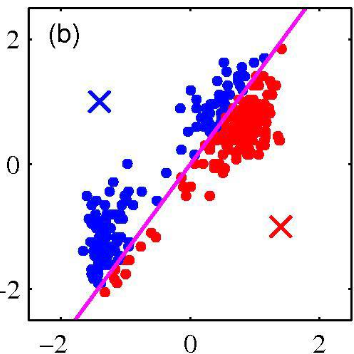
\includegraphics[width=0.58\textwidth]{img/kmeans2}
				\caption{Iterative step 1.}
			\end{minipage}        
			\hspace{2.5cm}
			\begin{minipage}[t]{0.42\linewidth} 
				\centering
				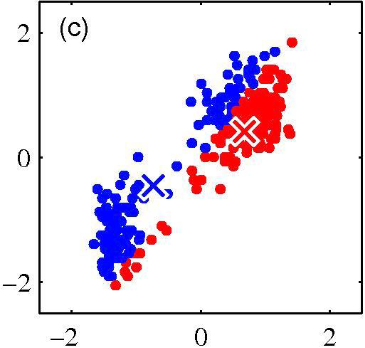
\includegraphics[width=0.58\textwidth]{img/kmeans3}
				\caption{Iterative step 2.}
			\end{minipage}
		\end{figure}
		\FloatBarrier
	\end{enumerate}
	\item \textbf{Stop:} when no points' assignments change.
	\begin{figure}[H]
		\begin{minipage}[t]{0.42\linewidth} 
			\centering
			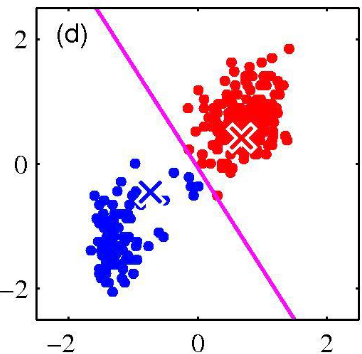
\includegraphics[width=0.58\textwidth]{img/kmeans4}
			\caption{Repeat until convergence.}
		\end{minipage}        
		\hspace{2.5cm}
		\begin{minipage}[t]{0.42\linewidth} 
			\centering
			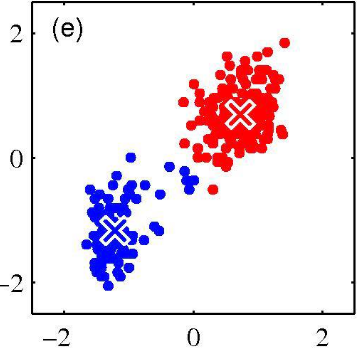
\includegraphics[width=0.58\textwidth]{img/kmeans5}
			\caption{Final output.}
		\end{minipage}
	\end{figure}
\end{itemize}
\paragraph*{Advantages of K-means.} 
\begin{itemize}
        \item It is a \textbf{simple algorithm};
	\item It is guaranteed to \textbf{converge} in a \textbf{finite number of steps};
	\item It \textbf{minimizes} an \textbf{objective function} (i.e. it \textbf{maximizes} the \textbf{compactness} of clusters):
	$$\sum_{i \in \text{clusters}} \Biggl\{ \sum_{j \in \text{elements of i-th cluster}} ||x_j - \mu_i||^2 \Biggr\}$$
	where $\mu_i$ is the center of cluster $i$;
	\item It \textbf{assigns} data points to closest cluster center in $O(Kn)$ and it \textbf{changes} the cluster center to the average of its points in $O(n)$, so it is an \textbf{efficient} algorithm.
\end{itemize}

\paragraph{Disadvantages of K-means}

\begin{itemize}
    \item It converges to a \textbf{local minimum} of the error function, i.e. we have no theoretical guarantees that the algorithm will converge to a global minimum, and that's the reason why we may run the algorithm several times;
    \item It needs to pick $K$ \textbf{initial points}, hence proving to be very \textbf{sensitive to the initialization step};
    \item It is also very sensitive to the \textbf{outliers}, which are not known in advance;
    \item It only finds \textbf{spherical clusters}, due to the objective function it minimizes. In this sense, this algorithm does not work when we have non-convex clusters;
    \item It works with \textbf{feature vectors}, which sometimes are not easy to obtain.
\end{itemize}

\subsection{Classification}
STL mainly deals with \textbf{supervised learning} problems: given an input (feature) space $\mathcal{X}$ and an output (label) space $\mathcal{Y}$ (typically $\mathcal{Y} = \{ +1, -1 \}$), the goal is to estimate a functional relationship between the input and output space:

$$
f: \mathcal{X} \xrightarrow{} \mathcal{Y}
$$

Usually, $f$ is called \textbf{classifier}, so a \textbf{classification algorithm} is a procedure that takes the training data ($(X_1, Y_1), .., (X_n, Y_n) \in \mathcal{X} \times \mathcal{Y}$) as input, and provides the classifier $f$ as output.

\subsubsection{Assumptions}
Moreover, SLT makes the following \textbf{assumptions}:

\begin{enumerate}
    \item There exists a joint probability distribution $P$ among $\mathcal{X} \times \mathcal{Y}$, which is usually not known;
    \item The training examples $(X_i, Y_i)$ are sampled i.i.d. from $P$.
\end{enumerate}

In particular, 

\begin{itemize}
    \item In STL, no assumptions are made on $P$, whereas in \textit{statistical inference} the data are assumed to follow a certain distribution;
    \item The distribution of $P$ is unknown at learning time;
    \item Non-deterministic labels due to label noise or overlapping classes;
    \item The distribution of $P$ is fixed, both during training and testing.
\end{itemize}

\subsubsection{Losses and risks}
Clearly, we need to have some measure of how good a function $f$ is when used as a classifier, so a \textbf{loss function} measures the "cost" of classifying instance $x \in \mathcal{X}$ as $y \in \mathcal{Y}$. 

In this sense, the simplest loss function is the \textbf{0-1 loss}, which is defined as:

$$
l(X,Y,f(X)) = \begin{cases}
    1 \qquad \text{if } f(X) \neq Y \\
    0 \qquad \text{otherwise}
\end{cases}
$$

We can define the \textbf{theoretical risk} of a function $f$ the average loss over data points generated according to the underlying distribution $P$:

$$
R(f) := \mathbb{E}(l(X,Y,f(X)))
$$

The \textbf{best classifier} is the one with the smallest risk $R(f)$: among all possible classifiers, the best one is the \textit{Bayes classifier}:

$$
f_{\text{Bayes}} := \begin{cases}
    1 \qquad \text{if } P(Y = 1 | X = x) \geq 0.5 \\
    -1 \qquad \text{otherwise}
\end{cases}
$$

Its idea is to classify the most frequent class. However, in practice it is impossible to directly compute the Bayes classifier, since the underlying distribution $P$ is unknown to the learner, and estimating $P$ from the data usually doesn't work.

Recall: Bayes' theorem says that:

$$
P(h|e) = \frac{P(e|h) P(h)}{P(e)} = \frac{P(e|h) P(h)}{P(e|h) P(h) + P(e|\Bar{h}) P(\Bar{h})}
$$
, where:

\begin{itemize}
    \item $P(h)$ represents the \textbf{prior probability} of hypothesis $h$;
    \item $P(h|e)$ represents the \textbf{posterior probability} of $h$ after the evidence $e$;
    \item $P(e|h)$ represents the \textbf{likelihood} of evidence $e$ on hypothesis $h$.
\end{itemize}

Returning to the classification problem, now the situation is that given:

\begin{itemize}
    \item A set of training data $(X_1, Y_1), .., (X_n, Y_n) \in \mathcal{X} \times \mathcal{Y}$ drawn i.i.d. from an \textit{unknown} distribution $P$;
    \item A loss function,
\end{itemize}

the goal is to determine a function $f: \mathcal{X} \to \mathcal{Y}$ which has a risk $R(f)$ which is as close as possible to the risk of the Bayes classifier. However, we notice that it is impossible to compute the risk of $f$ without knowing $P$..

\subsubsection{The nearest neighbor (NN) rule} A possible solution for this problem could be represented by the \textbf{nearest neighbor} approach, according to which the label of a data point $x$ is given by the label of the nearest point to $x$. Notice that in this case, no assumptions about the probability distribution of the data is used, since the method only uses information from the training set.

But, how good is the NN rule? It was showed that:

$$
R(f_{\text{Bayes}}) \leq R_{\infty} \leq 2R(f_{\text{Bayes}})
$$
, where $R_{\infty}$ denotes the expected error rate of NN when the sample size tends to infinity. Notice that we cannot say anything stronger about the bounds, since there are probability distributions for which the performance of the NN rule achieves either the upper or lower bound.

There exist some variations to the NN rule, for example the \textbf{$k$-NN} rule, which uses $k$ nearest neighbors and takes the majority vote, or the \textbf{$k_n$-NN rule}, which does the same, but for $k_n$ growing with $n$.

\textbf{Theorem (Stone, 1977)}: if $n \to \infty$ and $k \to \infty$, such that $k/n \to 0$ (i.e. $n$ grows faster than $k$), then for all probability distributions, $R(k_n - \text{NN}) \to R(f_\text{Bayes})$, i.e. the $k_n - \text{NN}$ rule is universally Bayes consistent.

However, all these NN rule have some \textbf{disadvantages}:

\begin{itemize}
    \item Not having a learning phase (\textit{lazy algorithm}), a huge amount of data must be kept in memory;
    \item They are very time demanding.
\end{itemize}

\subsection{Neural networks}
A Neural Network is an information processing paradigm that is inspired by the way biological nervous systems, such as the brain, process information. The key element of this paradigm is the new structure of the information processing system. It is composed of a large number of highly interconnected processing elements (\textbf{neurons}) working in unison to solve specific problems. A NN is configured for a specific application, such as pattern recognition or data classification, through a learning process.\\
Two key \textbf{features} distinguish neural networks from any other sort of computing developed:

\begin{itemize}
	\item \textbf{Neural networks are adaptive or trainable}. Neural networks are not so much programmed as they are trained with data. The more data they are fed, the more accurate or complete is their response;
	\item \textbf{Neural network are naturally massively parallel}. This suggests they should be able to make decisions at high-speed and be fault tolerant (information is stored in a distributed fashion). 
\end{itemize}

\subsubsection{The McCulloch and Pitts Model (1943)}

Neural network simulations appear to be a recent development; however, this field was established before the advent of computers and the first model, which was created in 1943, is the \textbf{McCulloch and Pitts Model}.\\
The McCulloch-Pitts (MP) neuron is a simple process unit modeled as a binary threshold unit.

\image{img/MP_neuron}{McCulloch and Pitts neuron representation.}{0.55}


\textbf{Input} = $x$ = $\sum_j w_jI_j$. \\
\textbf{Output} = $g(x) = \begin{cases}
0 \quad \text{if }x<T\\
1 \quad \text{if }x \geq T
\end{cases}$

In this sense, we can rewrite the output as:

$$
y = g\left(\sum_j w_jI_j - T\right) 
$$

\textbf{NOTE}:

\begin{itemize}
    \item the MP neuron fires if the input $x$ = $\sum_j w_jI_j$ exceeds a certain threshold $T$, called \textbf{claiming parameter};

    \item the function $g(.)$ is also called \textbf{activation function} or \textbf{unit step function}, and it is a non linear function;

    \item the weight $w_{ij}$ represents the strength of the synapse between neuron $i$ and neuron $j$. 
\end{itemize}

\subsubsection{Properties}

By properly combining MP neurons, it is possible to simulate the behavior of any boolean circuit:

\image{img/MP_properties}{Three elementary logical operations (\textit{a}) \textbf{negation}, (\textit{b}) \textbf{and}, (\textit{c}) \textbf{or}. In each diagram the states of the neurons on the left are at time $t$ and those on the right at time $t+1$.}{0.65}

Notice that it is not possible to build a NN for the \textit{XOR} operator using a single neuron.

\subsubsection{Network topologies and architectures} There are different network topologies and the main differences are highlighted below.

\begin{table}[H]
	\centering
	\begin{tabular}{| p{7.5cm} | p{7.5cm} |}
		\hline
		\textbf{Feed-forward only}: allow signals to travel one way only: from input to output, so it has connections only in one direction. This topology forms a direct acyclic graph, and its outputs are deterministic functions of the input & \textbf{Recurrent networks}: can have signals traveling in both directions by introducing loops in the network. Feedback networks are powerful and can get extremely complicated, since their output depends on the initial state, which in turn depends on previous outputs.\\
		\hline
		\textbf{Fully connected}: each neuron of a layer is connected to every neuron in the previous layer, and each connection has it's own weight. & \textbf{Sparsely connected}: has fewer links than the possible maximum number of links within that network.  \\
		\hline
		\textbf{Single layer}: every neuron connects directly from the network's input to its output & \textbf{Multi-layer}: it has one or more layer of hidden neurons that are not connected to the output.\\
		\hline
	\end{tabular}
\end{table} 
\image{img/feedforward}{\textit{(a)} feedforward network - \textit{(b)} feedback network}{0.65}

In general, there are problems which are more suited to be solved with a \textit{feedforward NN} than a \textit{recurrent NN} or vice-versa, for example a task of image classification, i.e. assigning a label to an input image, can be easily solved with a \textit{feedforward NN}, whereas a task of image captioning, i.e. provide a verbal description of the input image, is more suitable to be solved with a \textit{recurrent NN}, since the length of the output is not known in advance. 


\subsubsection{Classification problems}
Given:

\begin{enumerate}

	\item a set of \textbf{features} $\{f_1,f_2,\dots,f_n\}$ , which represents the attributes that describe our objects;
	\item a set of \textbf{classes} $\{c_1,\dots,c_m\}$, which represents the categories in which the objects are divided
 
\end{enumerate}

, the \textbf{goal} of the \textbf{classification} problem is to classify the \textbf{objects} according to their \textbf{features}. The geometric interpretation of this task is to represent the features in the space and try to separate the classes by finding the closest objects.

\image{img/nn1.jpg}{Classification problem}{0.7}

\subsubsection{Neural networks for classification}

A neural networks can be used as a classification device and it can be configured as follow:

\begin{itemize}

	\item the \textit{input} of the network are the object's \textbf{features} to classify.
 
	\item the \textit{output}, returned by the network, is the \textbf{class} predicted for the input object.
 
\end{itemize}

Before going on we assume that features are numbers, and remember that we cannot map categorical features into numbers, since we would introduce an order, which would lead to mistakes. For instance: red = 0, blue = 1, green = 2 would not be a correct coding since we would be imposing a non-existent order between colors. We propose a simple model of neural network:

\image{img/NN_1}{Example of NN with 3 features input and 2 class labels as output.}{0.4}

The application of a learning algorithm of a network configuration consists in finding the best configuration of weights of the incoming connection and the threshold. In these classification problems we can get rid of the \textbf{thresholds} (also called biases) associated to neurons by adding an extra input \textbf{permanently clamped at -1}. By doing so,\textbf{ thresholds become weights} and can be adaptively adjusted during learning phase, otherwise we would have to manually tune the right threshold. In this way, the output $y$ of the network becomes:

$$
y = g\left(\sum\limits_{i = 1}^{n+1} w_ix_i\right)
$$
, where $x_{n+1} = -1$.

\begin{figure}[h!]
		\centering
        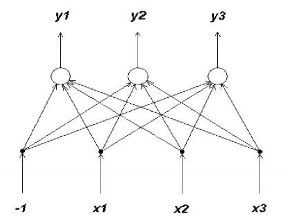
\includegraphics[scale = 1.5]{img/thresholds.jpg}
		\label{mi}
        \caption{We can remove thresholds by adding an input neuron clamped at -1}
\end{figure}

\subsubsection{The Perceptron}
The perceptron is a \textbf{linear classifier} consisting of a \textbf{single layer of MP neurons} connected in a \textbf{feedforward} way, i.e. it is a \textbf{single-layer feedforward NN}. A simple perceptron can only solve linearly separable problems, and this makes the model very limited in terms of computational power. 

\image{img/percep1.jpg}{Representation of a perceptron}{0.5}

The perceptron is characterized by the following properties:

\begin{itemize}
    \item The output is $-1/+1$, while using the MP neurons we had $0/1$;
    
    \item It is capable of learning from examples;
    
    \item From a geometrical point of view, the perceptron identifies a linear boundary between two classes:

    \image{img/percep2.jpg}{Geometry interpretation of the perceptron}{0.5}

    In this case, the hyperplane (line) $w_1x_1 + w_2x_2 + b$ represents a linear decision boundary for a two-dimensional, two-classes classification problem. If $w_1x_1 + w_2x_2 + b > 0$ then the predicted class is 1, otherwise is 0. Obviously, if we change the parameters $w_1$, $w_2$ and $b$, we get a different boundary.
    
\end{itemize}

\paragraph*{The Perceptron Learning Algorithm.} The goal of this algorithm is to find the best weights and parameters in order to separate the objects of the classes. It is an iterative algorithm characterized by the following variables and parameters:
\begin{itemize}

	\item $x(n) \in \mathbb{R}^{m+1}$, the \textbf{input vectors}. They are $(m+1)\text{-by-1 vectors} = [-1, x_1(n), x_2(n), \dots, x_m(n)]^T$\\
	Objects are described with $m$ features and -1 as the threshold, which is the reason why the input vectors have size $m+1$;
 
	\item $w(n) \in \mathbb{R}^{m+1}$, the \textbf{weights vectors}. They are $(m+1)\text{-by-1 vectors} = [b, w_1(n), w_2(n), \dots, w_m(n)]^T$;
 
	\item $b$, the \textbf{bias};
 
	\item $y(n)$, the \textbf{actual response} of the NN (quantized). $y(n) \in \{ +1, -1 \}$;
 
	\item $d(n)$, the \textbf{desired response} from the dataset. $d(n) \in \{ +1, -1 \}$;
 
	\item $\eta$, the \textbf{learning-rate parameter}, a positive constant strictly smaller than $1$. It affects the convergence of the learning algorithm. 
\end{itemize}

The algorithm works as follows:

\begin{enumerate}

	\item \textbf{Initialization.} Set $w(0) = 0$ and then perform the following computations for time-step $n=1,2,\dots$.
 
	\item \textbf{Activation.} At time-step $n$, activate the perceptron by applying continuous-valued input vector $x(n)$ and desired response $d(n)$ (both picked from the training set).
 
	\item \textbf{Computation of the actual response.} Compute the actual response of the perceptron as:
	$$y(n) = sgn[w^T(n)x(n)] \qquad w^Tx = \sum_iw_ix_i$$
	where $sgn(\cdot)$ is the signum function ($+1$ if the argument is greater or equal to $0$, $0$ otherwise). Notice that, so far, no learning phase has taken place.
 
	\item \textbf{Update of the weight vector.} Update the weight vector of the perceptron to obtain:
	$$w(n+1) = w(n) + \eta[d(n) - y(n)]x(n)$$
	where
	$$d(n) = 
	\begin{cases}
	+1 \qquad \text{if } x(n) \text{ belongs to class } \varphi_1\\
	-1 \qquad \text{if } x(n) \text{ belongs to class } \varphi_2 
	\end{cases}$$
	This is where the learning phase takes place: in case of wrong classification, the current configuration will change modifying $d(n) - y(n)$, if the network classifies $x(n)$ correctly, then there is no learning as $d(n)-y(n) = 0$. The convergence of the algorithm is ensured by $x(n)$. Note that $x(n)$ is included to be sure that the new prediction is correct, but the updated weights could fail to classify another input vector (even an already seen one).
 
	\item \textbf{Continuation.} Increment time step $n$ by one and go back to step 2.
 
\end{enumerate}

In practice, this algorithm is trying to find the best possible straight line (or hyperplane) which separates the ``good'' examples from the ``bad'' ones. The decision boundary is described such that $w_1x_1 + w_2x_2 = 0$ and, in general, each point is classified according to the following conditions:  $w_1x_1 + w_2x_2 \geq 0$ and $w_1x_1 + w_2x_2 < 0$

\image{img/perceptron_algorithm}{Perceptron learning algorithm procedure.}{0.50}

From a geometrical point of view, finding $w$ means finding the line (or hyperplane) which separates the two regions.
As we can see from the previous image, some examples can be misclassified. For each weights update, a specific error is corrected but other mistakes in classification may arise because of the changes in the weights. By iteratively adjusting the weights, a final and ``stable'' solution can be reached.\\
It is possible to define a \textbf{decision region} as an area in which all the samples of one class fall. A classification problem is said to be \textbf{linearly separable} if the decision regions can be separated by an hyperplane. These concepts allow us to introduce one important \textbf{limitation of perceptrons}: they can only solve linearly separable problems.

\paragraph*{The Perceptron Convergence Theorem.} This theorem was formulated by Rosenblatt in 1960. It states the following: if the training set is \textbf{linearly separable}, the perceptron learning algorithm \textbf{always converges} to a consistent hypothesis after a \textbf{finite} number of epochs, i.e. an entire presentation of the dataset, for any $\eta > 0$ (Note: nothing is said with respect to the number of steps).\\
If the training set is \textbf{not linearly separable}, after a certain number of epochs the weights will start oscillating. In this situation some points will surely be misclassified. The learning algorithm will never converge to a stable configuration, due to the fact that the perceptron can't solve non-linear classification problems.

\par \bigskip \noindent
\subsubsection{Multi-Layer Feed-forward Neural Networks}
In the following image it is possible to find some properties of the different structures that can create a neural network.

\image{img/role_units}{A view of the Role of Units}{0.86}

As we said before, the limit of the perceptron algorithm is that it can only deal with linearly separable problems. In order to overcome these limitations, the introduction of \textbf{multi-layer feed-forward networks} allows us to improve our networks through the addition of \textbf{hidden layers} between the input and the output layer. This allows us to reach a good approximation on our classification problem: it is possible to notice that a network with just one hidden layer can represent any Boolean function, including XOR. One property of such networks is the \textbf{universal approximation power}, which states that a 2-layers network (one input layer, one hidden layer) can approximate any smooth function (valid for regression problems), provided that the hidden layer is large enough.

\image{img/fNN.png}{Neural Network function model.}{0.65}		


\paragraph*{Continuous-valued units.} The usage of continuous-valued units allows us to introduce calculus and derivative procedures that will give us several advantages.\\ 
The \textbf{activation function} of continuous-valued units is \textbf{sigmoid} (or logistic), which means that neurons can now fire with different intensities, not only 0/1. In this sense, their output is not boolean, but it belongs to the continuous range between $0$ and $1$. These values are often interpreted as probabilities.
$$g \rightarrow \sigma(x) = \frac{1}{1+e^{-f(x)}} \in (0,1)$$
\image{img/sigmoid}{Sigmoid function.}{0.51}
Thus, continuous-valued discriminant functions allow us to have some measure of \textbf{confidence} about the \textbf{prediction}. We will see later on that they are used for \textbf{finding optimal solutions through the gradient descent technique}. In particular, when the $g(z)$ is close to zero (less confidence about the prediction) the gradient will be greater then the situation in which $|g(x)| >> 0$ (more confidence, weights could remain stable).

Another possible activation function is the \textbf{hyperbolic tangent} ($tanh$), which is a rescaling of the logistic sigmoid such that its output range is from -1 and 1. 
$$g \rightarrow \sigma(x) = \frac{e^{f(x)} - e^{-f(x)}}{e^{f(x)} + e^ {-f(x)}} \in (-1, 1)$$
\image{img/hyperbolic}{Hyperbolic tangent function.}{0.45}


\subsubsection{The Back-propagation learning algorithm}
In this section we introduce the \textbf{backpropagation}, an algorithm for learning the weights in a feed-forward multilayers neural network. 

Let $\mathcal{L} = \{(x_1, y_1), \dots, (x_n,y_n) \}$ be a \textbf{training set}, where $X = \{ x_1, x_2, .., x_n \}$ represents the network \textbf{input} vector and $Y = \{ y_1, y_2, .., y_n \}$ represents the \textbf{desired} network \textbf{output} vector. The algorithm is based on \textbf{gradient descent} method, and it can be seen as a greedy algorithm with infinite possible solutions, in which at each step the best solution is chosen. The algorithm is guaranteed to converge only to a local maximum and during the execution we move along the gradient through a predetermined step-size. This property is given by the fact that this algorithm is just an approximation based on a greedy solution.

\image{img/backpropagation}{Back-propagation schema. $W^l_{ij}$ represents the weight on connection between the $i^{th}$ unit in layer $(l-1)$ to $j^{th}$ unit in layer $l$.}{0.70}

\paragraph*{Supervised learning.} Supervised learning algorithms require the presence of \textbf{previous knowledge} that makes it possible to provide the \textbf{right answers} to the input ``questions''. Technically this means that we need a \textbf{training set} of the form:

$$
\mathcal{L} =\left\{\left(x^1, y^1 \right), \dots , \left(x^N, y ^N \right) \right\}
$$

where:

$$x^\mu (\mu=1,\dots, N) \text{ is the network \textbf{input} vector}$$
$$y^\mu (\mu=1,\dots, N) \text{ is the \textbf{desired} network \textbf{output} vector}$$

The learning (or \textbf{training}) phase consists in determining a configuration of \textbf{weights} such that the \textbf{network output} should be \textbf{as close as possible} to the \textbf{desired output} as many times as possible, for all the examples in the training set. Normally, this amounts to minimizing an \textbf{error function} such as the \textbf{MSE} (Mean Squared Error) function:
$$E(w) = \frac{1}{2} \sum_{\mu} \sum_{k} \left(y_k^\mu - O_k^\mu(w)\right)^2$$
where $O_k^\mu(w)$ is the \textbf{output} provided by the \textbf{output unit $k$} when the network is given example $\mu$ as \textbf{input}. In other words, $O_k^\mu(w)$ represents the prediction of the $k^{th}$ unit when the input is $\mu$. 

The loss function computes the difference between the network output and the expected output and of course, our aim is to \textbf{minimize the loss function} (i.e. solve $\min_w E(w)$), which means \textbf{finding the set of weights that minimizes the function}: if the network is performing well, then $E(w)$ is close to zero.

In order to minimize the error function $E$, we can use the classic \textbf{gradient descent} algorithm. The gradient gives information about the \textbf{best path to follow} in order to \textbf{maximize/minimize our objective function}. Without any kind of direction information it would be extremely complex to find the solution since we would have to search along an infinite number of directions in a continuous domain. Gradient descent is a very well-known \textbf{greedy algorithm}. It is not guaranteed to find a globally optimal solution, but it works well in finding \textbf{local optima}. 

More specifically, the gradient descent updates the a point by moving along the the direction given by the gradient by a finite step. In the case of the back-propagation algorithm, we have that:
$$w_{ji}^{\text{NEW}} \leftarrow w_{ji}^{\text{OLD}} - \eta \frac{\partial E}{\partial w_{ji}}$$

or

$$\Delta w_{ji} \leftarrow  - \eta \frac{\partial E}{\partial w_{ji}^{\text{OLD}}}$$

, where :

\begin{itemize}
    \item $\Delta w_{ji} = w_{ij}^{\text{NEW}} - w_{ji}^{\text{OLD}}$
    \item $w_{ji}^{\text{NEW}}$ represent the weights between unit $i$ and unit $j$, and they are updated using the gradient of the loss function $E$ computed w.r.t. $w_{ji}^{\text{OLD}}$;
    \item $\eta$ represents the \textbf{learning rate}, i.e. how much the weights are updated at each iteration of the gradient descent method. We will discuss about the possible values of this parameter later in the section;
\end{itemize}

Now we need to define a method for computing the partial derivatives of the loss function efficiently.

To compute the partial derivatives we use the \textbf{error back propagation} algorithm, which consists of two stages:

\begin{itemize}
	\item \textbf{Forward pass}: the \textbf{input} of the network is \textbf{propagated} layer after layer in \textbf{forward} direction.
	\item \textbf{Backward pass}: the \textbf{error} (e.g. MSE) made by the network is \textbf{propagated} \textbf{backward} and \textbf{weights} are \textbf{updated} properly. Thus, the partial derivatives of the errors are computed, and the weights are updated following the gradient descent strategy we defined above. An important thing to underline is that in order to update each weight, we only need a \textbf{local information}, not a global information of all the network.
\end{itemize}


Intuitively, we could say that we determine the gradient direction and then we move in the opposite direction since we want to minimize the error.

\paragraph*{Notation.} Before understanding how the weights are updated, it is important to introduce some notation that will be used later:

\begin{itemize}
    \item $x_k$ represents an input neuron of the network;
    \item $w_{jk}$ represents a weight between the input $x_k$ and the neuron $V_j$ in the middle layer;
    \item $V_j$ represents a neuron in the hidden layer;
    \item $W_{ij}$ represents a weight between a neuron in the hidden layer $V_j$ and the output neuron $O_i$;
    \item $O_i$ represents a output neuron.
\end{itemize}

\imageb{img/notations}{0.5}

Given a pattern $\mu$, an hidden unit $j$ receives a net input
$$h _ { j } ^ { \mu } = \sum _ { k } w _ { j k } x _ { k } ^ { \mu }$$
and produces as output:
$$V _ { j } ^ { \mu } = g \left( h _ { j } ^ { \mu } \right) = g \left( \sum _ { k } w _ { j k } x _ { k } ^ { \mu } \right)$$
The output of a neuron in the output layer is defined as:
$$O _ {i} ^ {\mu} = g(\sum _ k W_{ik} \cdot V _ {k} ^ {\mu})$$


\paragraph*{Updating hidden-to-output weights.} The \textbf{updating rules} of the back-propagation algorithm are nothing but a \textbf{long series of chain rules}. For this reason, the objective function is not linear, hence the output is highly non linear. Indeed, the output is a chain of products of non-linear functions.\\
\begin{equation} \notag
\begin{split}
\Delta W_{ij} &= -\eta \frac{\partial E}{\partial W_{ij}} \quad \text{Replace the error function with its actual expression}\\
&= -\eta \frac{\partial}{\partial W_{ij}} \left[\frac{1}{2} \sum_{\mu} \sum_k (y_k^\mu - O_k^\mu)^2\right] \quad \text{First application of the chain rule}\\
&= \eta \sum _{\mu} \sum_{k} \left(y_{k}^{\mu} - O_{k}^{\mu} \right) \frac{\partial O_{k}^{\mu}} {\partial W_{ij}} \quad \text{The sum over } k \text{ disappears because the partial derivative is}\\
& \hspace*{13.5em} \text{different from 0 only when }k=i \\
&= \eta \sum_{\mu} \left(y_{i}^{\mu} - O_{i}^{\mu} \right) \frac{\partial O_{i}^{\mu}} {\partial W_{ij}} \qquad \text{Again we apply the chain rule. Partial derivative can be}\\
& \hspace*{12.6em} \text{written as } W_{ij} \rightarrow h_i^\mu \rightarrow g'(h_i^\mu)\\
&= \eta \sum _ { \mu } \left( y _ { i } ^ { \mu } - O _ { i } ^ { \mu } \right) g ^ { \prime } \left( h _ { i } ^ { \mu } \right) V _ { j } ^ { \mu } \qquad \text{That is } \frac{\partial h_i^\mu}{\partial W_{ij}} = \frac{\partial}{\partial W_{ij}}\left(\sum_l W_{il} V_l \right) = V_j \frac{\partial W_{ij}}{\partial W_{ij}} = V_j\\
&= \eta \sum _ { \mu } \delta _ { i } ^ { \mu } V _ { j } ^ { \mu } \qquad \qquad where: \quad \delta _ { i } ^ { \mu } = \left( y _ { i } ^ { \mu } - O _ { i } ^ { \mu } \right) g ^ { \prime } \left( h _ { i } ^ { \mu } \right)
\end{split}	
\end{equation}
In $\eta \sum_{\mu} \delta_{i}^{\mu} V_{j}^{\mu}$, component $\delta_{i}^{\mu}$ represents the error made by the $i$-th neuron, whilst $V_{j}^{\mu}$ is the output of the neuron.  

\paragraph*{Updating input-to-hidden weights.}
\begin{equation} \notag
\begin{split}
\Delta w _ { j k } &= - \eta \frac { \partial E } { \partial w _ { j k } } \\
&= \eta \sum _ { \mu } \sum _ { i } \left( y _ { i } ^ { \mu } - O _ { i } ^ { \mu } \right) \frac { \partial O _ { i } ^ { \mu } } { \partial w _ { j k } } \qquad \text{Chain rule}\\
&= \eta \sum _ { \mu } \sum _ { i } \left( y _ { i } ^ { \mu } - O _ { i } ^ { \mu } \right) g ^ { \prime } \left( h _ { i } ^ { \mu } \right) \frac { \partial h _ { i } ^ { \mu } } { \partial w _ { j k } } \qquad \text{Chain rule}
\end{split}
\end{equation}
We have that the partial derivative is:
\begin{equation} \notag
\begin{split}
\frac { \partial h _ { i } ^ { \mu } } { \partial w _ { j k } } &= \sum _ { l } w_{ i l } \frac { \partial V _ { l } ^ { \mu } } { \partial w_{ j k } }\\
&= w_ { i j } \frac { \partial  V_ { j } ^ { \mu } } { \partial  w _ { j k } }\\
&= w_{ i j } \frac { \partial g \left( h _ { j } ^ { \mu } \right) } { \partial w _ { j k } }\\
&= w_{ i j } g ^ { \prime } \left( h _ { j } ^ { \mu } \right) \frac { \partial h _ { j } ^ { \mu } } { \partial w _ { j k } }\\
&= w_{ i j } g ^ { \prime } \left( h _ { j } ^ { \mu } \right) \frac { \partial } { \partial w _ { j k } } \sum _ { m } w _ { j m } x _ { m } ^ { \mu }\\
&=  w_{ i j } g ^ { \prime } \left( h _ { j } ^ { \mu } \right) x _ { k } ^ { \mu }
\end{split}
\end{equation}
Hence coming back to the original equation we have that:
\begin{equation}
\begin{split}
\Delta w _ { j k } &= \eta \sum _ { \mu , i } \left( y _ { i } ^ { \mu } - O _ { i } ^ { \mu } \right) g ^ { \prime } \left( h _ { i } ^ { \mu } \right) w_ { i j } ~g ^ { \prime } \left( h _ { j } ^ { \mu } \right) x _ { k } ^ { \mu }\\
&= \eta \sum _ { \mu , i } \delta _ { i } ^ { \mu } w_ { i j } g ^ { \prime } \left( h _ { j } ^ { \mu } \right) x _ { k } ^ { \mu }\\
&= \eta \sum _ { \mu } \hat { \delta } _ { j } ^ { \mu } x _ { k } ^ { \mu } \qquad \qquad where: \quad \hat { \delta } _ { j } ^ { \mu } = g ^ { \prime } \left( h _ { j } ^ { \mu } \right) \sum _ { i } \delta _ { i } ^ { \mu } w_ { i j }
\end{split}
\end{equation}
$\sum_{i} \delta_{i}^{\mu} W_{ij}$ is the average error performed by the output layer and $i$ is the reference to the $i$-th neuron.\\
In the following image it is possible to understand the error back-propagation. The black lines correspond to the forwarded signals, while the red lines indicate the error that is back-propagated.
\image{img/error_backpropagation}{Error Back-propagation representation.}{0.6}

\paragraph*{Locality of back-propagation.} Another important aspect is the \textbf{locality} of the back-propagation algorithm.

\image{img/locality_backpropagation}{Locality of back-propagation}{0.2}

There exist two different ways of implementing a back-propagation algorithm: off-line and on-line. In the \textbf{off-line} way we compute the gradient exactly, so in order to update a single weight in the network, we need to present all the examples of the training set. This procedure is not generally used because it is computationally expensive.

$$
\Delta \omega_{pq} = \eta \sum_{\mu} \delta_{p}^{\mu} V_{q}^{\mu} \qquad \qquad \text{off-line}
$$
$$
\delta_{p}^{\mu} = \text{Error} \quad V_{q}^{\mu} = \text{Output of neurons}
$$

In the \textbf{on-line} way some noise is introduced, in the sense that the weights are updated at any presentation of an example of the training set.

$$
\Delta \omega_{pq} = \eta\delta_ {p}^{\mu} V_{q}^{\mu} \qquad \qquad \text{on-line}
$$

A possible compromise between the two techniques is called \textbf{stochastic gradient descent}, in which the first technique is used with a randomly selected subset of the training set: in this sense, the gradient changes according to the random choice of the subset. This solution represents a very good method, since on the one hand modern datasets are huge, so updating the weights after the presentation of all the training examples is very expensive, and on the other the randomness through which the subset is selected may help in finding a global maximum/minimum.

\paragraph*{The Back-Propagation algorithm.} In this implementation we will consider the \textbf{on-line} approach. Suppose we have a network with $m$ layers, and let

\begin{itemize}
    \item $V_i^m$ be the output of the $i$-th unit of layer $m$;
    \item $w_{ij}^m$ be the weight on the connection between $j$-th neuron of layer $m-1$ and $i$-th neuron in layer $m$. 
\end{itemize}
  
The general structure of the algorithm is the following:

\begin{enumerate}
	\item Initialize the weight to (small) random values. The choice of small values is made to avoid the derivative of the logistic function being all zeros;
	\item Choose a pattern $\bar{x}^\mu$ and apply it to the input layer $(m=0)$, i.e.:
	$$V _ { k } ^ { 0 } = x _ { k } ^ { \mu } \qquad \forall k$$
	\item Propagate the signal forward (\textbf{Forward pass}):
	$$V _ {i} ^ { m } = g \left( h _ { i } ^ { m } \right) = g \left( \sum _ { j } w _ { i j } V _ { j } ^ { m - 1 } \right)$$
	\item Compute the $\delta$'s for the output layer (\textbf{Backward pass}):
	$$\delta _ { i } ^ { m } = g ^ { \prime } \left( h _ { i } ^ { m } \right) \left( y _ { i } ^ { m } - V _ { i } ^ { m } \right)$$
	\item Compute the $\delta$'s for all preceding layers (for each neuron):
	$$\delta _ { i } ^ { m - 1 } = g ^ { \prime } \left( h _ { i } ^ { m - 1 } \right) \sum _ { j } w _ { j i } ^ { m } \delta _ { j } ^ { m }$$
	\item Update connection weights according to the error, with learning rate $\eta$:
	$$w _ { i j } ^ { N E W } = w _ { i j } ^ { O L D } + \Delta w _ { i j } \qquad \text { where } \quad \Delta w _ { i j } = \eta \delta _ { i } ^ { m } V _ { j } ^ { m - 1 }$$
	\item Go back to step 2 until convergence, i.e. until $\Delta w _ { i j } = 0$. In real implementation we claim $||\Delta w _ { i j }||^2 < \epsilon$, or to stop after a finite number of epochs.
\end{enumerate}

One of the most challenging problems is the choice of the \textbf{learning rate} $\eta$. When $\eta$ is \textbf{small} the algorithm will converge but in a very \textbf{slow} way; on the other hand, when it is too \textbf{big}, there will be an \textbf{oscillating problem} that won't bring the algorithm to the convergence. \\
In the following image we can see the difference in convergence between the same algorithm run with different values of $\eta$. From left to right, they are $0.02, 0.0476, 0.049, 0.0505$.
\image{img/learning_rate}{The Role of the Learning Rate. The minimum is at the $+$ and the ellipse shows a constant error contour.}{0.9}
We can observe that the first case is too slow in reaching the minimum, while in the second and in the third case the oscillation becomes smaller and smaller. Finally, in the last case, the algorithm won't converge, as the oscillation becomes larger and larger.\\

One possible remedy to this problem is in introducing the \textbf{momentum term}, a simple \textbf{heuristic} that can help in finding a good value for $\eta$. This improvement has the advantage of introducing a correction that is based on the step at time $t-1$, while the original algorithm produces a correction which is only related to the current point.
$$\Delta \omega_{pq}(t+1) = -\eta \frac{\partial E}{\partial w_{pq}}+\underbrace{\alpha \Delta w_{pq} (t)}_{\text{momentum }}$$

\begin{itemize}
	\item If $\alpha = 0$ we come back to the original formula $\Delta = f(w^T)$
	\item Otherwise $\Delta = f(w^T, w^{t-1})$
\end{itemize}
The momentum term introduces \textbf{dependency} on the previous step. The obvious disadvantage is the need to \textbf{set two parameters instead of one}. On the other hand the momentum term \textbf{allows} us to \textbf{use large values} of $\eta$ avoiding the introduction of the oscillatory phenomena. The application of the momentum term can be seen in the following image.
\image{img/momentum_term}{Momentum term application.}{0.45}
Both trajectories use $\eta=0.0476$ that is the best value of learning rate in the absence of momentum. In the left example, no momentum is applied $(\alpha=0)$, while in the right one we have $\alpha=0.5$. The application of momentum, hence, brings a clear improvement in convergence.

\paragraph*{The problem of local minima.} One of the toughest disadvantages to overcome is the fact that back-propagation cannot avoid the \textbf{problem of local minima}., i.e. the fact that the solution provided by the gradient descent approach is not global but only local.

\image{img/problem_local_minima}{The problem of local minima.}{0.4}

For this reason the \textbf{choice} of \textbf{initial weights} is of uttermost importance. If the weights are too large, the non-linearities tend to saturate since the beginning of the learning process. \\
A common heuristic for the choice of the initial weights is: 
$$w_{ij} \simeq 1/\sqrt{k_i}$$
, where $k_i$ is the number of units that feed unit $i$ (the "fan-in" of $i$)

\paragraph*{NETtalk.} \textbf{NETtalk} represents an example of application of the Back-propagation algorithm. This model is composed by a Neural Network and a speech synthesizer, and its goal is to pronounce the string that is provided as input to the network. In this case, each of the letter in input is represented using one-hot-encoding: there are 203 input units encoding the letters and 1 hidden layer with 80 units, while the output units encode English phonemes.

The model was trained by 1024 words in context, and it was able to produce intelligible speech after 10 training epochs, resulting to be functionally equivalent to DECtalk, an expert system, with the difference that this model does not require any linguistic knowledge.

\subsubsection{Theoretical and practical questions}
\begin{itemize}
	\item How many layers are needed for a given task? If the problem is linearly separable, than 1 layer is enough (Perceptron), otherwise we also noticed that 2 layers are enough to solve any problem, provided that the layers are large enough, which sometimes is unfeasible.
	\item How many units per layer should we use?
	\item To what extent does representation matter?
	\item What do we mean by generalization?
	\item What can we expect from a network as far as generalization is concerned?
	\begin{itemize}
		\item \textbf{Generalization:} it can be defined as the \textbf{performance} of the network on \textbf{data} \textbf{not} included in the \textbf{training set}. One of the major \textbf{advantages} of neural nets is their ability to \textbf{generalize}, i.e. to classify data (belonging to the same class as the learning data) that it has never seen before. To reach the best generalization, the dataset should be split into three parts: \textbf{training set}, \textbf{validation set} and \textbf{test set}.\\
		The learning should be stopped when the minimum of the validation set error is reached. At this point the net should be generalizing in the best possible way. When learning is not stopped, ``overtraining'' occurs and the performance of the net on the dataset as a whole decreases, despite the fact that the error on the training data still gets smaller. In this case, we say the network is \textit{overfitting}. As a matter of fact, after finishing the learning phase the net should be evaluated on the third data set, the test set.
		\item Size of the training set: how large should a training set be for "good" generalization?
		\item Size of the network: too many weights in a network may result in poor generalization.
	\end{itemize}
\end{itemize}

\subsection{Model evaluation}
When we talk about model evaluation, it is important to understand how the performance of a model can be evaluated. An intuitive idea is that the \textbf{lower} the \textbf{error} generated by the model is, the \textbf{better} the \textbf{model} is. In this sense, it is possible to discern between two different types of errors:
\begin{itemize}
	\item The \textbf{true error} (denoted as $error_{\mathcal{D}}(h)$) of hypothesis $h$ with respect to target function $f$ and distribution $\mathcal{D}$, is defined as the probability that $h$ will misclassify an instance drawn at random according to $\mathcal{D}$.
	$$error_{\mathcal{D}}(h) \equiv \operatorname{Pr}_{x \in \mathcal{D}} \left[f(x) \neq h(x)\right]$$ 
	In other words, the true error measures the probability of making a mistake in real life. However, notice that for computing this quantity it is necessary to have knowledge of the probability distribution, which is usually unknown;
	
	\item The \textbf{sample error} (denoted as $error_{s}(h)$) of hypothesis $h$ with respect to target function $f$ and data sample $S$ is:
	$$error_{S}(h) \equiv \frac{1}{n} \sum_{x \in S} \delta (f(x) , h(x))$$ 
	, where $n$ is the number of examples in $S$, and the quantity $\delta(f(x), h(x))$ is $1$ if $f(x) \neq h(x)$, and $0$ otherwise. The sample error comes from the idea of estimating the probability distribution of the data from the samples available.
\end{itemize}

The \textbf{true error} is \textbf{unknown} (and will remain so forever), while in order to compute the sample error, it is possible to split the dataset, keeping a percentage for the training set and a percentage for the test set. Once the model is trained, it is evaluated over the test set, i.e. by measuring its error on unseen data. Clearly, a good choice of the training set and the test set is crucial.

\image{img/train_test}{Training set vs Test set.}{0.4}

\paragraph{Cross-Validation} Cross-validation is a technique that avoids the chance that the choice of the test and training sets affect the model evaluation. This technique is based on iteratively splitting the dataset into a number of training and test folds such that at each iteration the model is both trained and evaluated considering different examples of the dataset.

\image{img/cross_validation}{Cross validation example using
\textbf{leave-one-out} technique, i.e. the size of the test fold is 1.}{0.6}

Clearly, the \textbf{advantage} of this method is that it provides a very accurate measure of the error of the model, but on the other hand the drawback is its complexity in time when the datasets are large.

\paragraph{Overfitting}
Even though cross-validation can give us a good evaluation of the model, it is possible that this score could be affected of \textbf{overfitting}. 

\image{img/overfitting}{Example of overfitting.}{0.65}

In the image \textbf{(a)}, we notice a good fit to noisy data and the model seems to be using fewer parameters to capture the general behavior. In image \textbf{(b)}, instead, an overfitted model can be seen: the fit is perfect on the training set, but it is likely to be poor on the test set represented by the circle, i.e. it is characterized by a poor generalization power. \textbf{Occam's razor} intuitively explains why the simplest model is to be preferred.\\
The different steps in the model definition are reached through the separation of the starting set in:
\begin{itemize}
	\item \textbf{Training set:} to train the learning algorithm;
	\item \textbf{Validation set:} to stop the learning algorithm. In particular, it is used to evaluate whether the model is facing overfitting or not by measuring the error on unseen data. In this sense, its functioning is very similar to the test set, but the usage is different, since in this case its goal is to measure the minimum error in order to decide the stopping time;
	\item \textbf{Test set:} to evaluate the performance of the learning algorithm.
\end{itemize}
\image{img/early_stopping}{Early stopping.}{0.5}
Epochs of a machine learning algorithm represent the steps taken by the algorithm. Starting from the green line (overfitting line), the model will start to overfit on the training data. Notice also that the global optimum consists in an overfitted model, with the error function approaching zero.
The learning algorithm is stopped when the fit starts deteriorating.

\paragraph*{Size of a Neural Network} 
The size of a NN, i.e. the number of hidden neurons, affects both its functional capabilities and its generalization performance.
\begin{itemize}
	\item A \textbf{big network} leads to poor generalization performance and to the phenomenon of overfitting;
	\item A \textbf{small network} could not be able to model the desired input/output mapping and for this reason it would not actually learn anything. This phenomenon is called underfitting.
\end{itemize}

In general, it is hard to tell when the algorithm should stop because it is impossible to foresee if increasing the number of neurons would significantly decrease the error. This problem is known as the \textbf{horizon effect}. A common strategy is called \textbf{growing}: the procedure starts with one neuron and trains it. Going on, it will iteratively add neurons until satisfying results are obtained.
\section{Face Detection} \label{ch2}

The \textbf{face detection} problem is an instance of the general object detection problem, and its goal is to \textbf{identify and locate human faces in images or videos}, regardless of their position, scale, pose, orientation illumination etc..

\begin{figure}[h!]
		\centering
		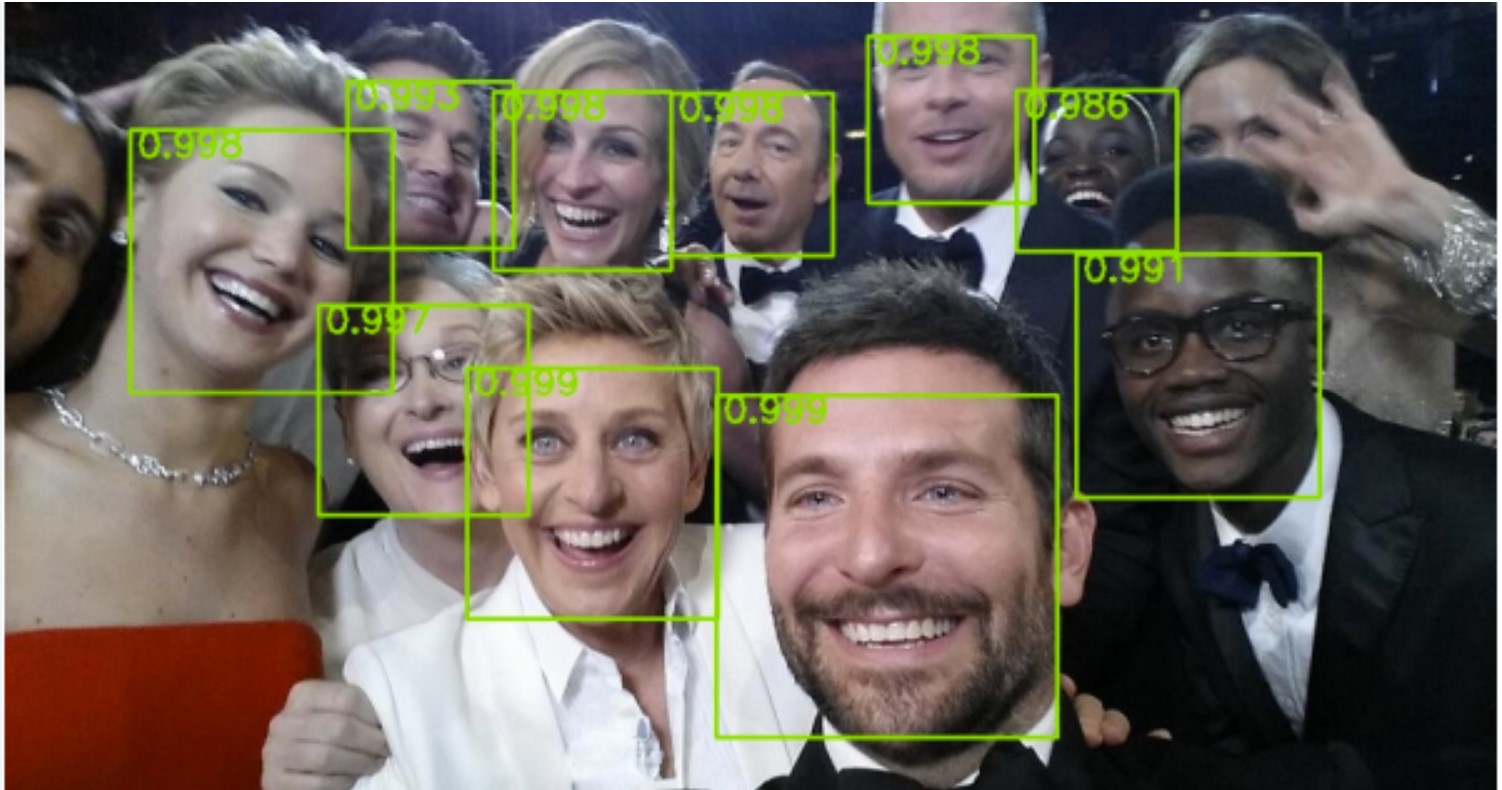
\includegraphics[scale = 0.7]{img/face detection.jpg}
        \caption{Face detection problem}
\end{figure}

If we consider a thumbnail $19$x$19$ face pattern, then there are $256^{231}$ possible combinations of gray values, i.e. $2^{2888}$, which is something like 87 times more than the world population, indicating an extremely high dimensional space! In this sense, the main difficulties of this problem rely on:

\begin{itemize}
    \item the different \textit{scales} of the images;
    \item the different \textit{poses} of the humans in an image;
    \item the problem of \textit{occlusion};
    \item the different \textit{expressions};
    \item \textit{Illumination}.
\end{itemize}

Moreover, there have been examples of images that fooled a \textit{face detection} algorithm.

\begin{figure}[h!]
		\centering
		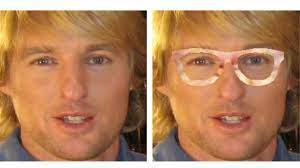
\includegraphics[scale = 0.7]{img/fool.jpeg}
        \caption{Example of image that fools a face detection algorithm}
\end{figure}

\subsection{Related problems}
As we introduced before, the \textit{face detection} problem represents an instance of the more general \textit{object detection} problem, and in turn there exist some related problem to the \textit{face detection}'s one:

\begin{itemize}
    \item \textit{Face localization}, i.e. determine the position of a single face, assuming that the image contains only one face;
    \item \textit{Facial feature extraction}, i.e. detect the presence and locations of features such eyes, nose etc..;
    \item \textit{Face recognition}, i.e. compare an input image, called probe, against a database, called gallery, and report a match. Note that this problem is different from face detection, since in the latter we are not asked to recognize the face: in general, \textit{recognition} is concerned with individual identity, while \textit{detection} with the category of an object;
    \item \textit{Face authentication}, i.e. verify the claim of the identity of an individual in an input image;
    \item \textit{Face tracking}, i.e. continuously estimate the location and possibly the orientation of a face in an image sequence in real time;
    \item \textit{Emotion recognition}, i.e. identifying the affective states (happy, sad, disgusted, etc.) of humans;
\end{itemize}

\subsection{Research issues}
The main issues of \textit{face detection} problem are:

\begin{itemize}
    \item \textbf{Representation}, i.e. how to describe a typical face;
    \item \textbf{Scale}, i.e. how to deal with faces of different scales;
    \item \textbf{Search strategy}, i.e. how to spot the faces;
    \item \textbf{Speed}, i.e. how to speed up the process of spotting;
    \item \textbf{Precision}, i.e. how to locate the faces precisely;
    \item \textbf{Post-processing}, i.e. how to combine detection results.
\end{itemize}

\subsection{Methods}
There exist various methods that are used to address the \textit{face detection} problem, and the most important ones are described below:

\begin{itemize}
    \item \textbf{Knowledge-based methods}: these methods are based on the idea of encoding the human knowledge of what constitutes a typical face (usually the relationships between facial features), and then build a detection algorithm based on these rules. This approach is not related with ML, so it is basically composed of IF-THEN-ELSE;
    \item \textbf{Feature invariant approaches}: in this case the focus is on finding features of a face that are invariant with respect to the pose, the illumination etc.. Still no ML;
    \item \textbf{Template matching methods}: they store several standard patterns to describe the face as a whole or the facial features separately;
    \item \textbf{Appearance-based methods}: these methods exploit the Neural Networks to learn the models (or templates) which capture the representative variability of facial appearance.
\end{itemize}

In the following sections we will provide an analysis of all the methods described above.

\subsubsection{Knowledge-based methods}
As we introduced before, the goal of these methods is to encode the relationships between facial features, i.e. the eyes, the nose etc.., in order to build a detection algorithm based on these rules. In this sense, we can recognize a \textbf{top-down} approach, since the detection is based on a set of human-coded rules. Some examples of these rules are:

\begin{itemize}
    \item the center part of face has uniform intensity values;
    \item the difference between the average intensity values of the center part and the upper part is significant;
    \item a face often appears with two eyes that are symmetric to each other, a nose and a mouth.
\end{itemize}

We analyze two different \textit{knowledge-based methods}: the first one was proposed by \\ \cite{YANG199453}, while the second one by \\ \cite{kotropoulos1994nonlinear}.

\underline{\textbf{Yang and Huang, 1994}}: this algorithm was based on a multi-resolution focus-of-attention approach. In particular,

\begin{itemize}
    \item the \textbf{Level 1}, i.e. the slowest resolution, applied the first rule described above in order to search for candidates;
    \item the \textbf{Level 2} produced a local histogram equalization, in order to correct the image in case of light issues etc.., followed by edge detection;
    \item finally, the \textbf{Level 3} was responsible for searching the eyes and the mouth features for validation.
\end{itemize}

\underline{\textbf{Kotropoloulos and Pitas, 1994}}: the idea of this algorithm was to perform both horizontal and vertical projections of the input image in order to search for candidates. The projections were computed as:

$$
HI(x) = \sum_y I(x,y)
$$

$$
VI(y) = \sum_x I(x,y)
$$

Then, the intersection of these two projections allowed to detect the face. However, it was difficult to detect multiple objects or people in complex background.

In general, the main \textbf{advantage} of this method is that it is quite easy to come up with simple rules to describe the features of a face and their relationships, so for this reason this kind of algorithms are simple to be implemented. Moreover, they obtain really good results for face localization in uncluttered background. On the other hand, the main \textbf{disadvantage} of this approach is that both detailed and general rules to detect faces may find many false positives, and in general it is difficult to extend this approach to detect faces in different poses.

\subsubsection{Feature invariant approaches}
While \textit{knowledge-based methods} follow a top-down approach for detecting faces on an image by following some human-coded rules, the \textit{feature invariant methods} follow a \textbf{bottom-up} approach. Their goal is indeed to detect invariant facial features (for example the eyes, the nose etc..), 
 then to group them into candidates and, finally, to verify them. Since the features are not random, they can be represented as a graph, where the edges represent the relationships between them: in this sense, the \textit{face detection} problem turns into a \textit{graph matching} problem!

 An example of algorithm following this approach was implemented by \\ \cite{leung1995finding}. 
 
 \underline{\textbf{Leung et al, 1995}}: in his solution, he formulated the \textit{face detection} problem as a problem of finding the correct geometric arrangement of facial features, where the facial features were defined by the average responses of multi-scale filters. Finally, the result was given by a graph matching among the candidates to locate faces.

In general, the main \textbf{advantage} of this approach is that, in contrast with the \textit{knowledge-based methods}, in this case the features are invariant to the pose and the orientation changes. On the other hand, two \textbf{disadvantages} of this method are that it is difficult to locate facial features due to several corruption (for example, illumination, noise etc..), and to detect features in complex backgrounds.

\subsubsection{Template matching models}
This approach is similar to the previous one, since its goal is to store one or more hand-coded templates and to use the correlation between the templates and the image in order to locate faces. The templates can be either predefined, i.e. they are based on edges or regions, or deformable, i.e. they are based on facial contours, so they adapt to different faces. Pictures \ref{predefined} and \ref{deformalble} represents, respectively, an example of predefined and deformable templates: as we can see, in both cases the goal of the algorithm is to find some points in the image that match with the template.

\begin{figure}[h!]
		\centering
		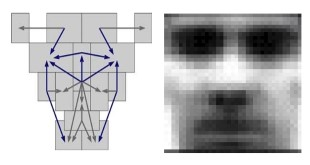
\includegraphics[scale = 1.5]{img/predefined.jpg}
        \label{predefined}
        \caption{Example of predefined template}
\end{figure}

\begin{figure}[h!]
		\centering
		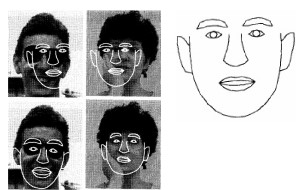
\includegraphics[scale = 1.5]{img/deformable.jpg}
        \label{deformalble}
        \caption{Example of deformable template}
\end{figure}

In general, these algorithms are simple, but on the other hand they need the templates to be initialized near the face images, and it is difficult to enumerate all the possible templates for different poses (similarly to knowledge-based methods)

\subsubsection{Appearance-based methods}
The last family of methods we analyze are the \textit{appearance-based methods}, which are the only ones characterized by a ML (or data driven) approach. The general idea of these algorithms is to:

\begin{enumerate}
    \item Collect a large set of (resized) face and non-face images and to train a binary classifier to discriminate them;
    \item Given a test image, they detect faces by applying the trained classifier at each position and scale of the image
\end{enumerate}

Note that the second phase ensures that the algorithms are invariant to different positions and scales. We will analyze three different algorithms: the first one was introduced by \cite{sung1998example}, the second one by \\ \cite{rowley1998neural}, while the third one by \cite{viola2001rapid}.

\underline{\textbf{Sung and Poggio, 1994}}: the main idea of this algorithm is to exploit the sliding window approach. In particular, the sliding window moves across the image running a classifier in order to detect if the portion contains an image or not. Note that this technique is repeated for different sizes of the image, in order to make it invariant to scale. Moreover, as mentioned before, the \textit{appearance-based methods} exploit the functioning of the Neural Networks, and in this case the \textit{back-propagation}  technique was exploited. Overall, the algorithm was composed of several phases, which are described below, while Picture \ref{poggio_overview} represents an overview of the algorithm.

\begin{figure}[h!]
		\centering
		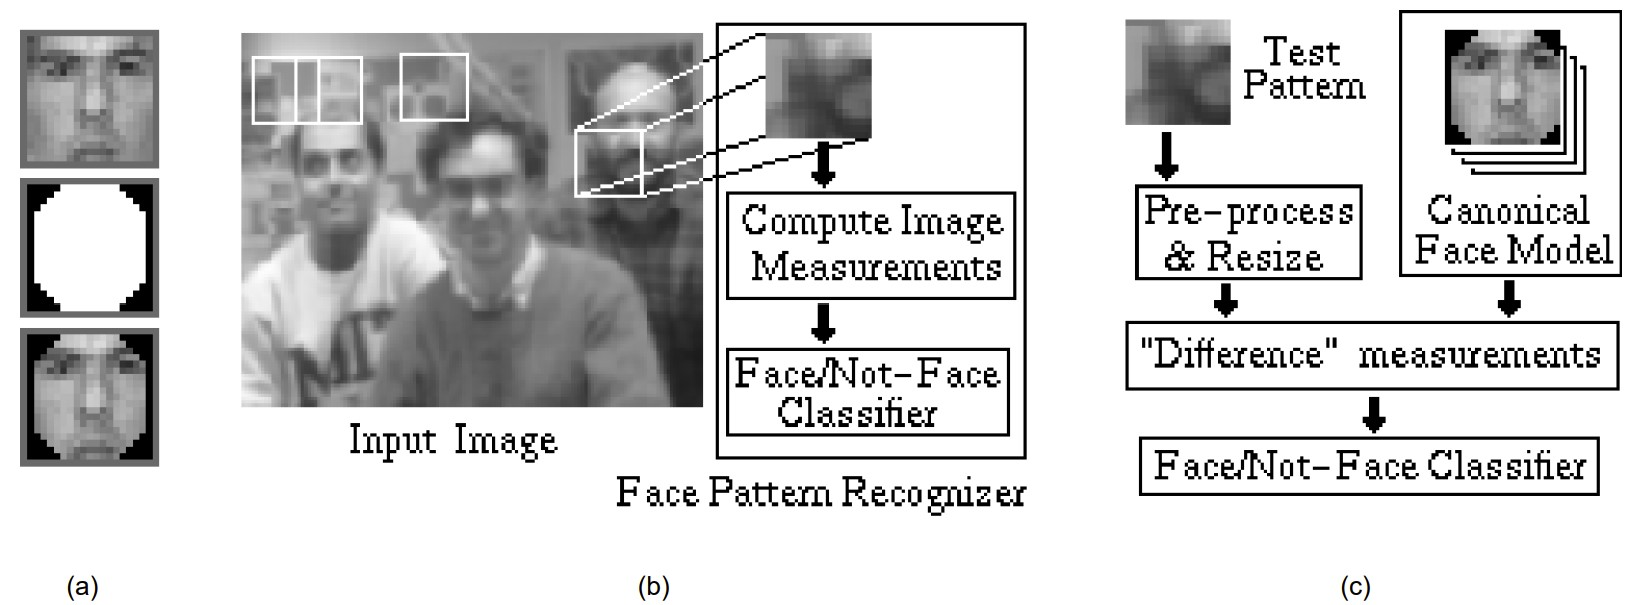
\includegraphics[scale = 0.7]{img/poggio_overwiew.jpg}
        \label{poggio_overview}
        \caption{Overview of the algorithm}
\end{figure}

\begin{enumerate}
    \item \textbf{Pre-processing phase}: in this phase the input image is "cleaned" in the following steps:
    \begin{itemize}
        \item \textbf{Resizing}, i.e. all the image patterns are resized to 19x19 pixels;
        \item \textbf{Masking}, which reduces the unwanted background noise in a face pattern. This is done by using an oval mask, and not a rectangular one, exploiting the fact that the face in the image does not fill the corner of a rectangular mask;
        \item \textbf{Illumination gradient correction}, which finds the best fit brightness plane and then subtract from it to reduce heavy shadows caused by extreme lightning angles. This step is done for solving face detection problem for images with shadows;
        \item \textbf{Histogram equalization}, which compensates the imaging effects due to changes in illumination and different camera input gains.
    \end{itemize}
    
    \item \textbf{Modeling the distribution of "face" and "non-face" patterns}: now the goal is to classify each portion of the image, and this is done by building a training set composed by both positive examples and negative examples (always 19x19 images). Then the idea was to consider these examples as points, and to cluster these points into \textbf{6 different clusters} by using $K Means$ algorithms, in order to group faces with similar expression (they estimated in 6 the number of different expression of a human face). Each cluster is modeled by a multi-dimensional Gaussian with a centroid and a covariance matrix, and each Gaussian covariance is approximated with a subspace, i.e. by using the largest eigenvectors. A visual representation of this phase is provided in Picture \ref{poggio_clusters}.

    \begin{figure}[h!]
		\centering
		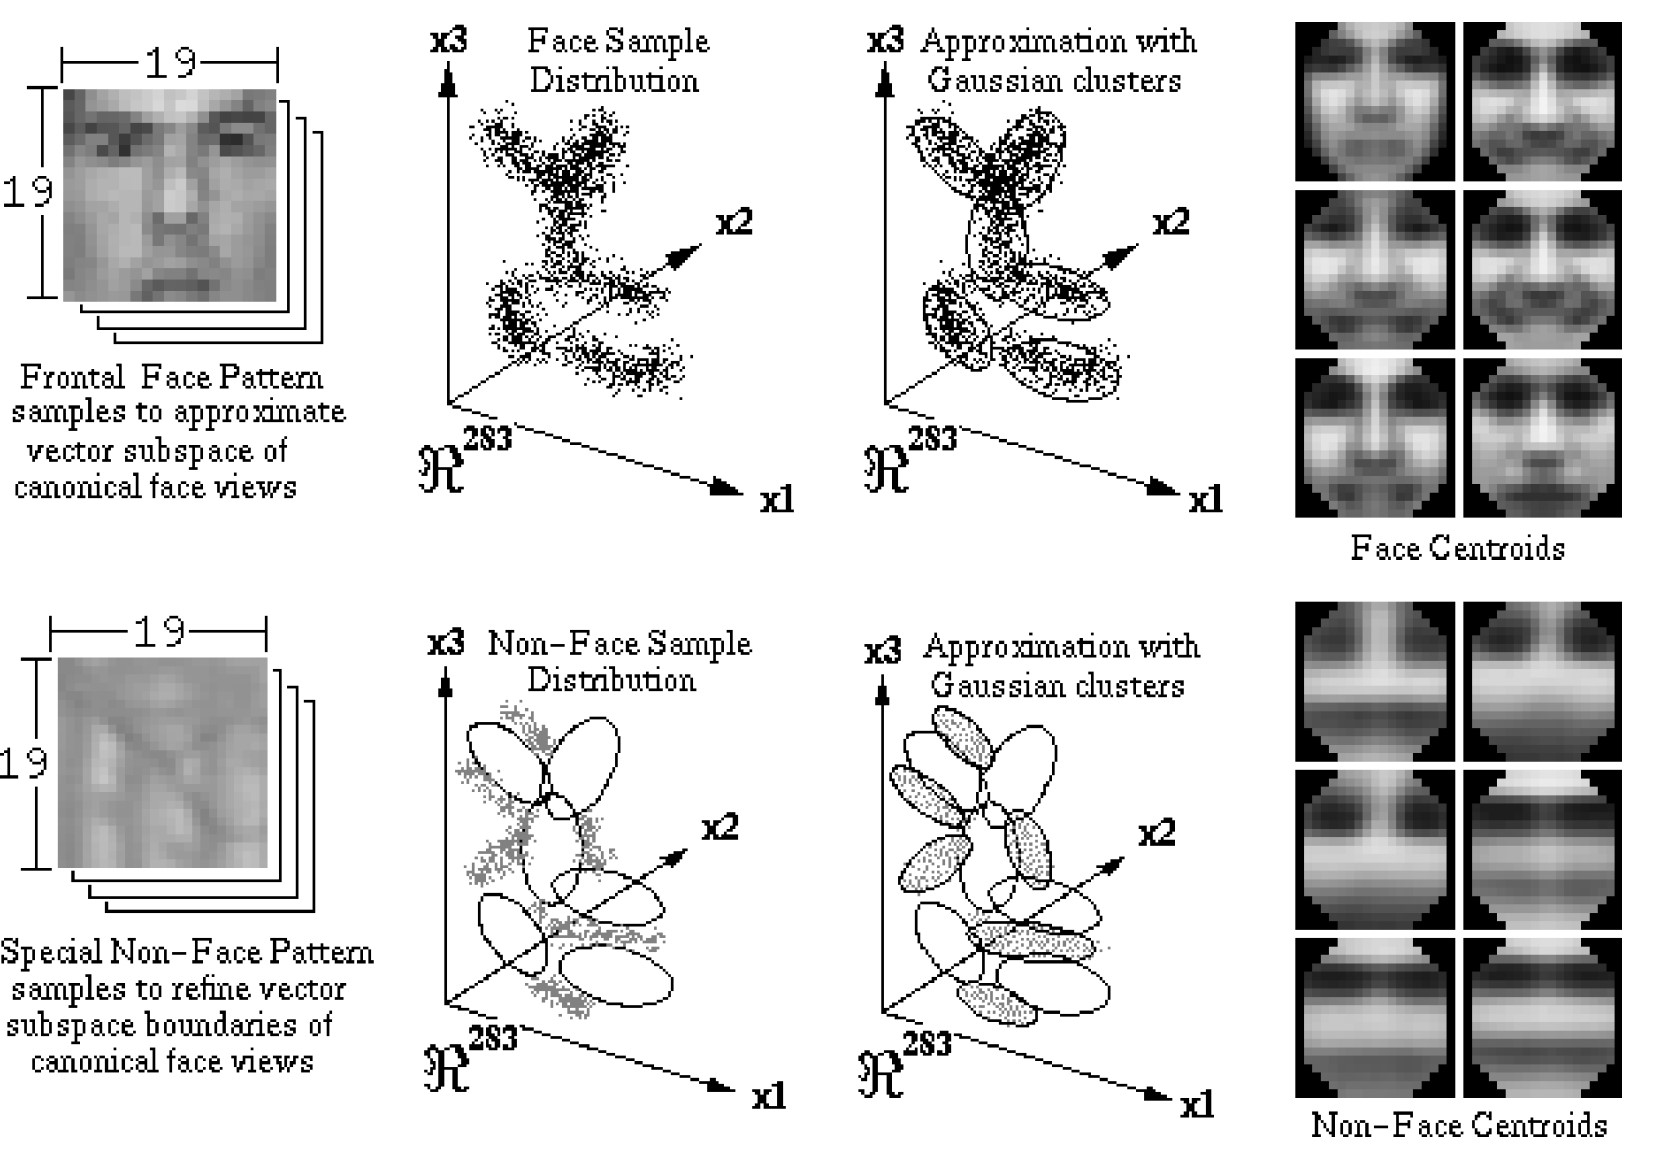
\includegraphics[scale = 0.7]{img/poggio_clusters.jpg}
        \label{poggio_clusters}
        \caption{Second phase of the algorithm}
    \end{figure}

    \item \textbf{Matching patterns with the model}: to detect faces in an input image, the system matches window patterns at different image locations and scales against the distribution-based face model. Before each match, the system first applies the preprocessing operations to the current window pattern. Each match returns a \textbf{set of “difference” measurements} which is fed to a trained classifier that determines whether or not the current window pattern is a frontal face view. More specifically, each set of measurements is a \textbf{feature vector of 12 distances} between the normalized input window pattern and the model’s 12 cluster centroids in our multidimensional image vector space, as represented in Picture \ref{poggio_measurements}. 

    \begin{figure}[h!]
		\centering
		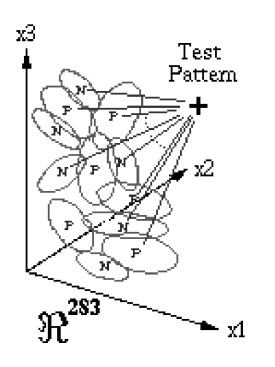
\includegraphics[scale = 1.2]{img/poggio_measurements.jpg}
        \label{poggio_measurements}
        \caption{Set of "difference" measurements}
    \end{figure}

    Moreover, each of the 12 distances is composed of two parts:

    \begin{itemize}
        \item the \textit{within subspace distance} $D_1$, which is represented by the Mahalanobis distance between the projected sample and the cluster centroid;
        \item the \textit{distance to the subspace} $D_2$, which is represented by the distance between the sample and the subspace.
    \end{itemize}

    A visual representation of $D_1$ and $D_2$ is provided in Picture \ref{poggio_distance}.

    \begin{figure}[h!]
		\centering
		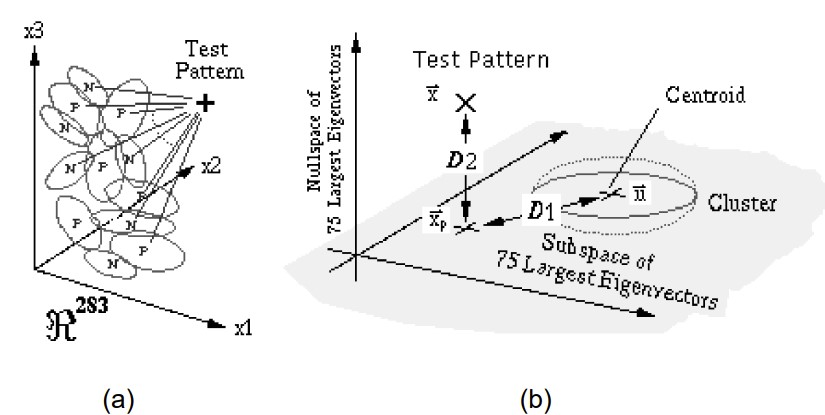
\includegraphics[scale = 1.2]{img/poggio_distance.jpg}
        \label{poggio_distance}
        \caption{Visual representation of $D_1$ and $D_2$}
    \end{figure}

    \item \textbf{The classifier}: the final phase of the algorithms is the classification phase. A \textbf{Multi-layer Neural Network} is used to identify "face" windows patterns from "non face" patterns by using the feature vector of 12 distances derived from the previous phase. The network has:

    \begin{itemize}
        \item 12 pairs of input units, each of which representing a pair $(D_1,D_2)$ of distances;
        \item 24 hidden units (it was proved that this number does not significantly affect the network's performance);
        \item 1 output unit ("face" or "non face").
    \end{itemize}

    During classification, the net is given a vector of the current test pattern’s distance measurements to the 12 cluster centroids: the output unit returns a 1 if the input distance vector arises from a “face” pattern, and a 0 otherwise. The net was trained on feature distance vectors from a database of 47,316 window patterns containing 4,150 positive examples of “face” patterns with a standard \textbf{back-propagation learning algorithm} until the output error stabilizes at a very small value.

\end{enumerate}

A crucial aspect of this algorithm is that the feature vector was not chosen from the image, but it was built by using a set of distances from the test patterns: in this sense, the Neural Network worked as a Nearest Neighbor classifier. Another important issue of this method was the \textbf{generation of the training set}. As we described above, the training set was composed by both positive and negative examples: for "face" patterns the selection was quite simple, because the simply collected all the possible views of human faces. However, since the collection of "face" patterns was not so large, their idea was to increase it by creating some \textbf{virtual examples}, each of which was derived by randomly mirror, rotate, translate and scale the original "face" examples. This technique is called nowadays \textbf{data augmentation}. Picture \ref{poggio_virtual} shows some virtual examples.

\begin{figure}[h!]
		\centering
		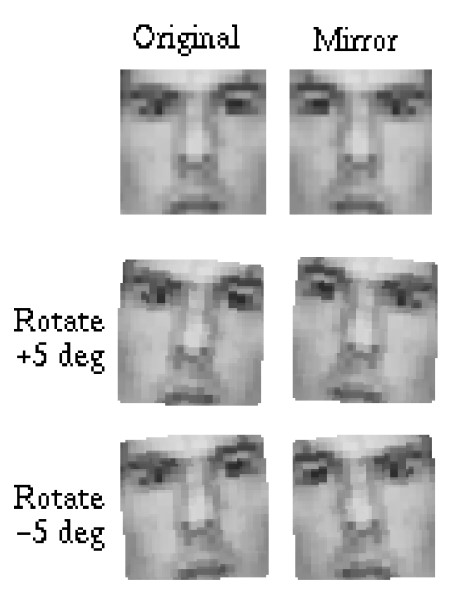
\includegraphics[scale = 1.0]{img/poggio_virtual_examples.jpg}
        \label{poggio_virtual}
        \caption{Virtual examples}
\end{figure}

For “non face” patterns, the task is more tricky. In essence, every square non-face window pattern of any size in any image is a valid training example. Clearly, our set of “non face” patterns can grow intractably large if we are to include all possible “non face” patterns in the training set. To constrain the number of “non face” examples in the training set, they used the following \textbf{bootstrap} strategy that incrementally selects only those “non face” patterns with high utility value with the following steps:

\begin{enumerate}
    \item Start with a random small set of "non face" examples in the training set;
    \item Train the Neural Network classifier with the current training set;
    \item Run the learned face detector on a sequence of random images;
    \item Collect all the "non face" patterns that the current detector wrongly classified as faces, i.e. the false positives;
    \item Add these "non faces" patterns to the training set;
    \item Repeat from 2 until satisfied.
\end{enumerate}

Note that this technique leads to two important consequences: the first one is that it provides a simple method to build "non faces" patterns, and the second one is that the training set is enlarged with examples that steer the classifier away from its current mistakes.

Finally, one last feature of this algorithm is that in order to be invariant to different scales, the input images were downsampled by a certain scaling factor. Picture \ref{poggio_results} shows a result of the algorithm.

\begin{figure}[h!]
		\centering
		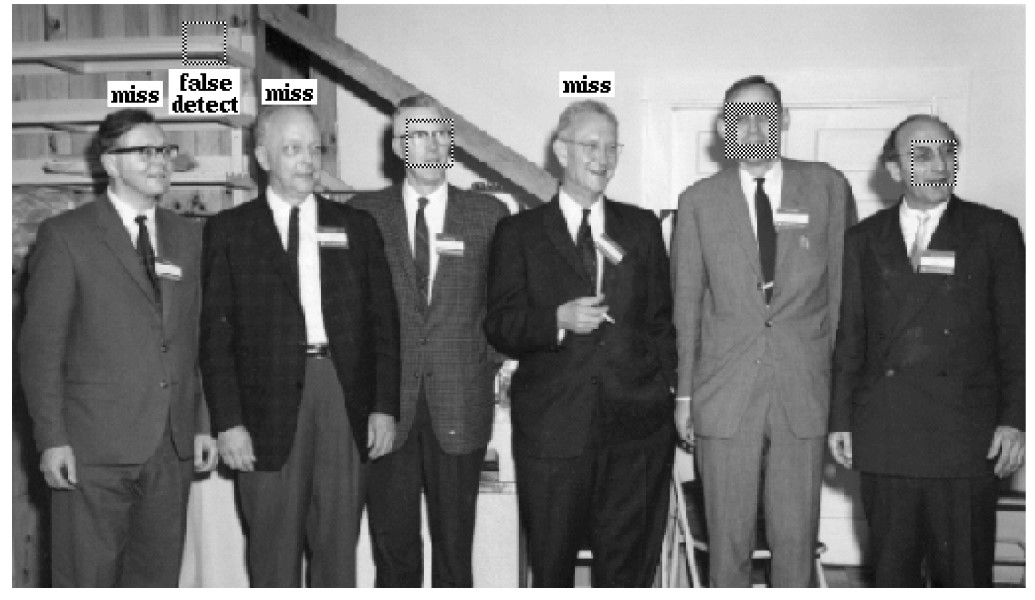
\includegraphics[scale = 1.0]{img/poggio_results.jpg}
        \label{poggio_results}
        \caption{Results of the algorithm}
\end{figure}

\underline{\textbf{Rowley-Baluja-Kanade (1996)}}: this algorithm is much similar to what we do nowadays, and the main difference with the previous one relies on the way in which the Neural Network is used, while the pre-processing and the other phases are quite similar. Picture \ref{rowley_overview} represents an overview of the algorithm.

\begin{figure}[h!]
		\centering
		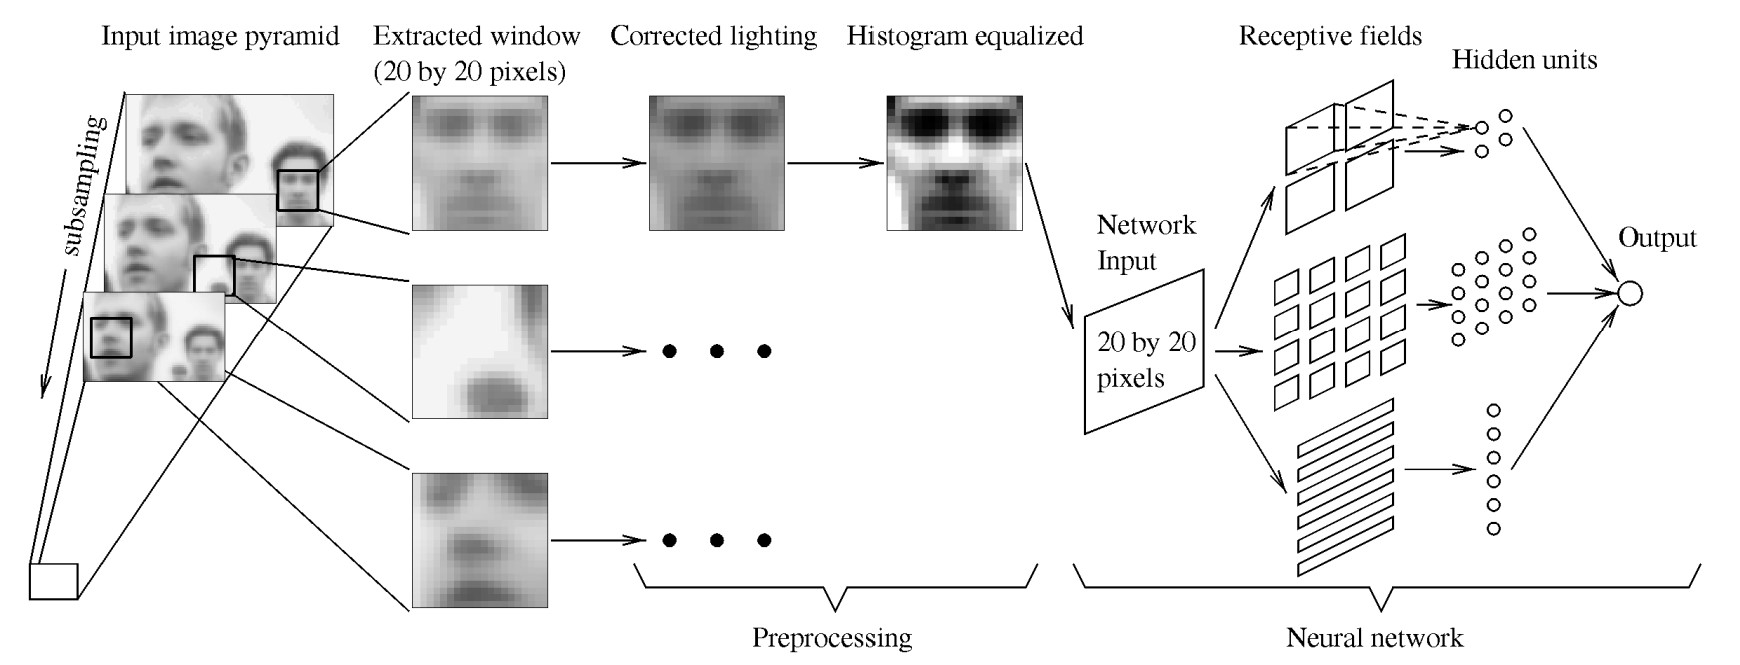
\includegraphics[scale = 0.7]{img/rowley_overview.jpg}
        \label{rowley_overview}
        \caption{Overview of the algorithm}
\end{figure}

As we can see, the pre-processing phase is very similar to the previous algorithm, with the only difference with the size of the patterns, which is now 20x20 (the previous one was 19x19). As we said before, the main difference relies in the \textbf{Neural Network}: in this case the features were extracted directly from the image, and they exploited the concept of \textbf{receptive field} of a neuron. While in a standard Neural Network, each neuron receives in input all the outputs of the neurons in the previous layer, in a Neural Network with receptive fields, each hidden unit receives in input the outputs of a subset of neurons of the previous layer, as showed in Picture \ref{receptive}. 

\begin{figure}[h!]
		\centering
		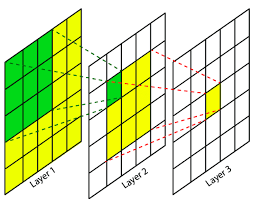
\includegraphics[scale = 0.5]{img/receptive_field.png}
        \label{receptive}
        \caption{Representation of the functioning of the receptive field of a neuron}
\end{figure}

In this sense, in this algorithm the input patch was splitted in several sub-regions, each of which was "controlled" by different neurons. The size of the receptive fields of the hidden unit were different, in order to detect local features that could be important for the problem of face detection. In particular, the hidden units with horizontal receptive fields were able to detect such features as mouths or pairs of eyes, while the hidden units with square receptive fields were able to detect features such as individual eyes, the nose, or corners of the mouth. 

The overall performances of this algorithm were better than Sung and Poggio, and in general their results were astonishing at that time. In Picture \ref{rowley_results} we provide an example of result of this algorithm.

\begin{figure}[h!]
		\centering
		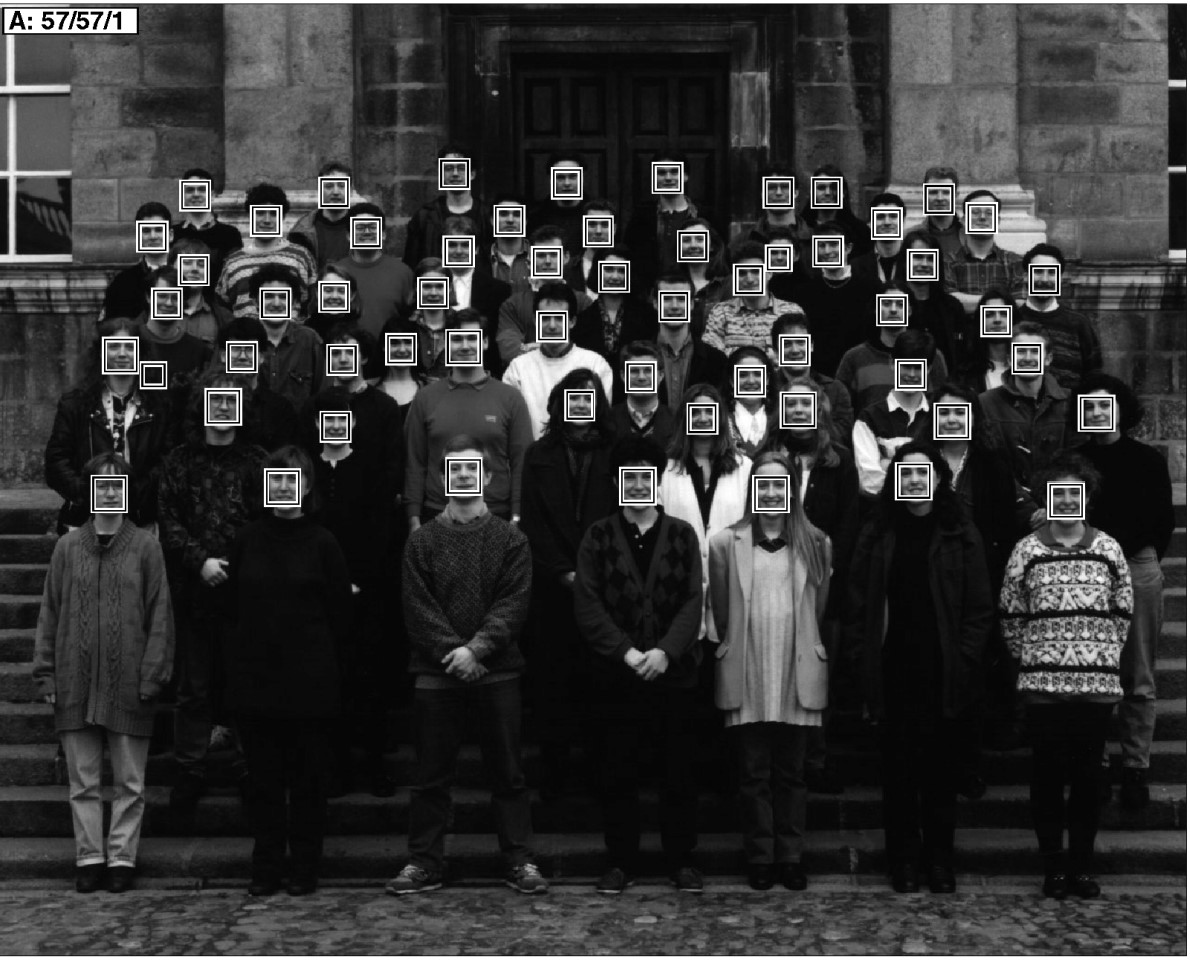
\includegraphics[scale = 0.6]{img/rowley_results.jpg}
        \label{rowley_results}
        \caption{Results of the algorithm}
\end{figure}

However, in 1998 the same authors provided a new version of the algorithm \\ (\cite{rowley1998rotation}) which was able to detect \textbf{rotated faces}. The idea for solving this new problem was the following one: before feeding the face detector, they built a Neural Network, called \textit{Router Network} which was trained to estimate the rotation angle of the input window. If the window contained a face, the the \textit{Router} returned the angle of the face and the face was rotated back to upright frontal position, otherwise it returned a meaningless angle. Then, the de-rotated window was applied to the face detector, which was previously trained for upright frontal faces. Picture \ref{rowley_rotated} represents an overview of this second version of the algorithm.

\begin{figure}[h!]
		\centering
		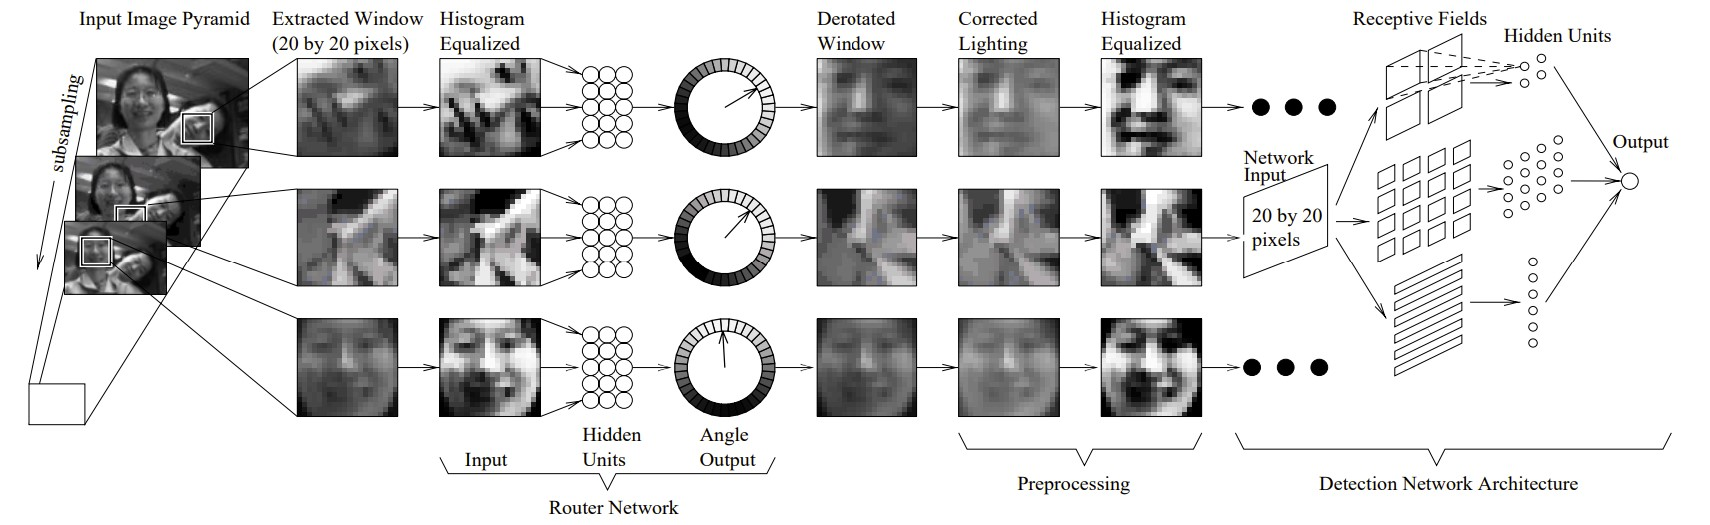
\includegraphics[scale = 0.8]{img/rowley_overview_rotated.jpg}
        \label{rowley_rotated}
        \caption{Overview of the new version}
\end{figure}

In order to implement these operations, the training set for the \textit{Router Network} was built by exploiting the so-called \textbf{self learning} technique, which avoids to manually label the whole training set. The value of the rotation angle for each image was not manually added, but it was retrieved by rotating the original upright image by a certain value, which therefore was added in the training set. 

Despite being much more accurate that Sung and Poggio, this algorithm had still some problems with the accuracy, and, especially, it had unacceptable CPU times.

\underline{\textbf{Viola and Jones, 2001}}: this algorithm represented the first real-time face detector, and for this reason it was implemented in real systems for a long time. It was characterized by a slow training phase, while the detection phase was very fast; in general, the three main contributions of this work were:

\begin{enumerate}
    \item A new image representation called \textbf{integral image}, which allows the features used by the detector to be computed in a very fast way;
    \item A learning algorithm, based on \textit{AdaBoost}, for feature selection: it selects a small number of critical visual features from a larger set and yields extremely efficient classifiers;
    \item A method, called \textbf{attentional cascade}, for fast rejection of non face windows. The idea was to use sliding windows, but without wasting any time in a non face portion of the image.
\end{enumerate}

Now we focus on each of the three contributions. In general, the object detector was based on very \textbf{simple features}: they used \textit{two-rectangle features}, \textit{three-rectangle features} and \textit{four-rectangle features}, as represented in Picture \ref{viola_features}.

\begin{figure}[h!]
		\centering
		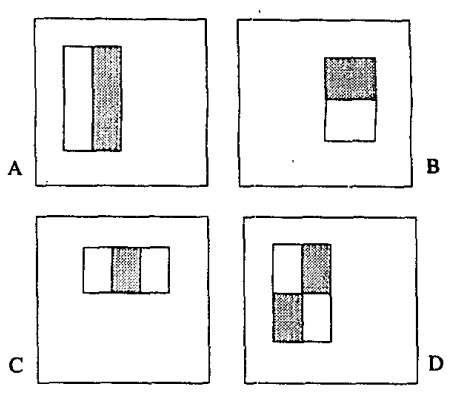
\includegraphics[scale = 1.2]{img/viola_features.jpg}
        \label{viola_features}
        \caption{Rectangular features}
\end{figure}

Each of the features computed the sum of the values in the white area subtracted by the sum of the values in the black area. In this way, the value of the feature was maximum if all the relevant pixels of the underlying portion of the image were positioned under the white area of the rectangle. An example is represented in Picture \ref{viola_features_2}.

\begin{figure}[h!]
		\centering
		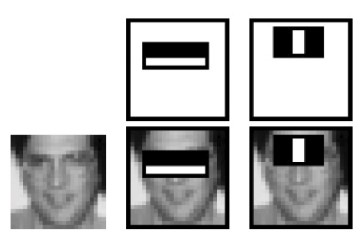
\includegraphics[scale = 1.2]{img/viola_features2.jpg}
        \label{viola_features_2}
        \caption{Features and an image}
\end{figure}

Moreover, the rectangle features can be computed very quickly using an intermediate representation of the image that is called \textbf{integral image}. The \textit{integral image} computes a value at each pixel $(x,y)$ as the sum of the pixel values above and to the left of $(x,y)$ inclusive, i.e.

$$
ii(x,y) = \sum_{x' \leq x, y' \leq y} i(x',y')
$$
, where $i(x',y')$ corresponds to the original image. An important property of the \textit{integral image} is that it can be computed in a single pass over the image, i.e. in linear time, by considering the following pair of recurrences:

$$
s(x,y) = s(x-1,y) + i(x,y)
$$

$$
ii(x,y) = ii(x,y-1) + s(x,y)
$$
, where $s(x,y)$ represents the cumulative sum of the row values.
In this sense, we can exploit this important property in order to compute in linear time the sum of the values of the rectangular features. For example, if A,B,C and D are the values of the \textit{integral image} at the corners of a rectangle, then the sum of the original image values in the rectangle is given by A-B-C+D. As we can see, only three additions are required for any size of the rectangle, which make the feature extraction a very fast operation. Notice that for a 24x24 detection region, which was the region used in the model, the number of possible rectangle features is around 180,000.

Then, the second important innovation of the algorithm was about the \textbf{learning algorithm} adopted both for the feature selection phase and to train the classifier, which was based on the \textbf{ensemble approach}. While in a standard ML pipeline a single complex learning algorithm is trained with the training set and tested with the test set, in the \textit{ensemble approach} a family of weak algorithms is trained, and the prediction is taken from the majority vote or the average of the predictions of all the weak algorithms. Note that a "weak learner" needs only to do better than chance, i.e. better than a model that predicts by tossing a coin. The functioning of this approach is represented in Picture \ref{ensemble}.

\begin{figure}[h!]
		\centering
		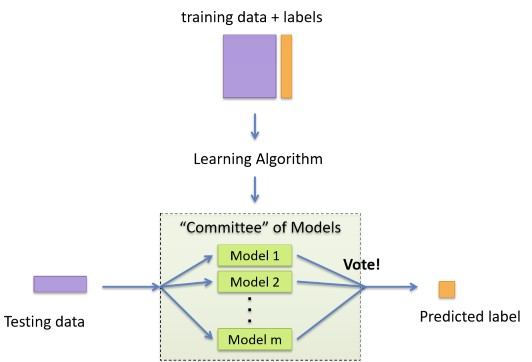
\includegraphics[scale = 1.4]{img/enseble.jpg}
        \label{ensemble}
        \caption{Functioning of the ensemble methods approach}
\end{figure}

One example of algorithms exploiting this idea of the \textit{ensemble methods} is the \textbf{Boosting} algorithm: in this case each weak model is trained sequentially, and the instances that are misclassified by a model are given more weight, i.e. more attention, so that the following model focuses more on classifying correctly those instances.

\begin{figure}[h!]
		\centering
		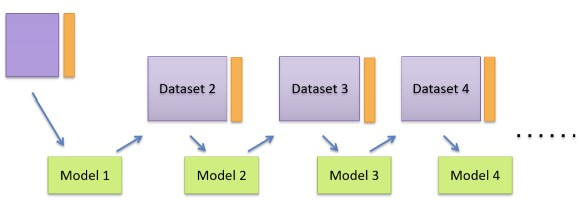
\includegraphics[scale = 1.4]{img/boosting.jpg}
        \label{boosting}
        \caption{Boosting algorithm}
\end{figure}

In particular, the \textit{Boosting} algorithm can be summarized as follows:

\begin{enumerate}
    \item Initially, all the weights of the training set are equal;
    \item In each boosting round, the weak learner that achieves the lowest weighted error in chosen, and the weights of the training examples that are misclassified by this learner are risen;
    \item The final classifier is computed as a linear combination of all weak learners, where the weight of each learner is directly proportional to its accuracy.
\end{enumerate}

The exact formulas for re-weighting and combine the weak learners depend on the particular boosting scheme (e.g. \textit{AdaBoost}). 

As we said before, even though each of the rectangular feature could be computed very efficiently by exploiting the \textit{integral image} representation, computing the complete set of 180,000 features was prohibitively expensive. Their hypothesis was that a very small number of these features could be combined to form an effective classifier, so the \textit{feature extraction} phase was implemented using the \textit{ensemble approach} define above. More specifically, for each feature, the weak learner determines the optimal threshold classification function, such that the minimum number of examples are misclassified. From a mathematical point of view, the learner is defined as:

$$
h_j(x) = \begin{cases}
	1 \qquad \text{if } p_jf_j(x) < p_j\theta_j\\
	0 \qquad \text{otherwise}
	\end{cases}
$$
, where:

\begin{itemize}
    \item $x$ is a 24x24 window of the image;
    \item $p_j$ is a parity bit, i.e. it is equal to 1 if we impose the feature to be greater than the threshold, -1 otherwise;
    \item $f_j(x)$ is the response of the rectangle feature, computed using the \textit{integral image};
    \item $\theta_j$ is the thershold.
\end{itemize}

Finally, Picture \ref{adaboost} represents the \textit{AdaBoost} algorithm which was implemented for both feature selection and training the classifier.

\begin{figure}[h!]
		\centering
		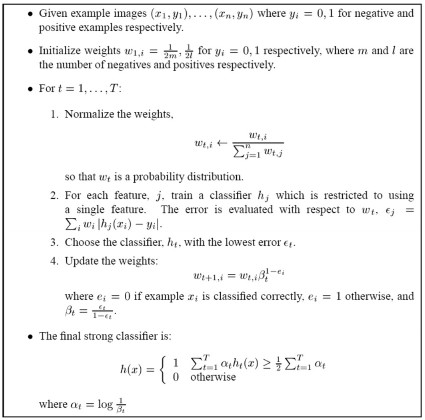
\includegraphics[scale = 1.8]{img/adaboost.jpg}
        \label{adaboost}
        \caption{AdaBoost algorithm}
\end{figure}

Some notes:

\begin{itemize}
    \item The training set is composed of both positive and negative examples;
    \item The weights are initialized uniformly;
    \item Point 2. computes the error of the learner w.r.t. the feature $j$: notice that $|h_j(x_i) - y_i|$ represents the actual error of the learner, while $w_i$ represents the weight of the example;
    \item Point 4. updates the weights of the examples: notice that $\beta_t < 1$, so if the example is correctly classified, then its weight is reduced, otherwise it remains the same. However, since the weights are normalized, this reduction will lead to an increase of the weights of the misclassified examples.
\end{itemize}

The first feature that was selected seemed to focus on the property that the region of the eyes is often darker than the region of the nose and cheeks , while the second selected feature relied on the property that the eyes are darker than the bridge of the nose. This feature combination could yield almost 100\% detection rate and 50\% false positive rate. Moreover, it was proved that a 200-features classifier could yield to a 95\% detection rate with a false positive rate of 1 in 14084; however, adding features to the classifier directly increases the computation time.

The last crucial idea developed in this model was the method of \textbf{attentional cascade}, whose goal was to construct a cascade of classifiers which achieves increased detection performance while radically reducing computation time. The key idea is that smaller, and therefore more efficient, boosted classifiers can be constructed in order to reject many of the negative sub-windows while detecting almost all positive instances. Simpler classifiers are used to reject the majority of sub-windows before more complex classifiers are called upon to achieve low false positive rates. A visual representation of this method is provided in Picture \ref{cascade}.

\begin{figure}[h!]
		\centering
		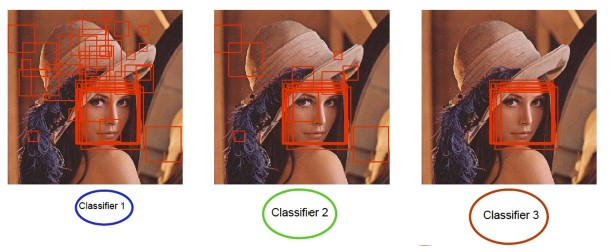
\includegraphics[scale = 1.8]{img/cascade.jpg}
        \label{cascade}
        \caption{Attentional cascade}
\end{figure}

 As we can see, the first classifier sees all the possible sub-windows, but a negative outcome at any point leads to the immediate rejection of the sub-window, which is therefore not considered by the following, a more complex classifier. In the case of the \textit{attentional cascade} method, both the detection rate and the false positive rate are computed by multiplying the respective rates of the individual stages: in general, it was proved that a detection rate of $0.9$ and a false positive rate of $10^{-6}$ can be achieved by a 10-stage cascade if each stage has a detection rate of $0.99$ and a false positive rate of $0.30$. Two possible problems about the \textit{attentional cascade} approach can be either that a classifier rejects a sub-window in which there's a face or that several detections are found for a single face. In particular, the second issue is shared among all the appearance-based methods we discussed, and it can be solved by applying the \textit{non-maximum suppression} method, which is implemented as follows:

 \begin{itemize}
     \item The set of detections are first partitioned into disjoint subsets: two detections are in the same subset if their regions overlap;
     \item Each partition yields a single final detection, whose corners are the average of the corners of all detections in the subset.
 \end{itemize}

A visual result of the application of the \textit{non-maximum suppression} method is provided in Picture \ref{nms}.

\begin{figure}[h!]
		\centering
		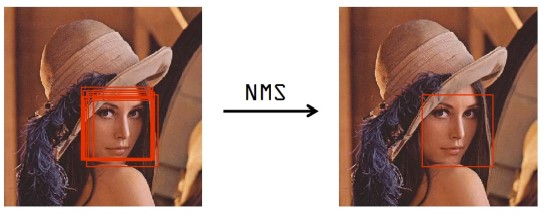
\includegraphics[scale = 1.8]{img/nms.jpg}
        \label{nms}
        \caption{Result of non-maximum suppression process}
\end{figure}

The \textit{Viola and Jones} algorithm was trained with 4,916 hand labeled faces and 10,000 non faces, containing many variations (illumination, pose etc..). The training phase took several weeks, and the final detector contained 38 layers for a total of 6,061 features. The test time was 15 times faster that \textit{Rowley-Baluja-Kanade}.

\section{Human Detection} \label{ch3}
The goal of the \textbf{human detection} problem is to detect and localize persons in an image regardless of their position, scale, pose, orientation and illumination.

\begin{figure}[h!]
		\centering
		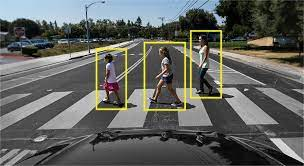
\includegraphics[scale = 0.7]{img/pedestrian recognition.jpeg}
        \caption{Pedestrian recognition problem}
\end{figure}

The main difficulties of this problem are:

\begin{itemize}
    \item The wide variety of articulated \textit{poses};
    \item Variable \textit{appearance and poses};
    \item Complex \textit{background};
    \item \textit{Occlusion};
\end{itemize}

\subsection{Research issues}
The main issues of \textit{pedestrian recognition} problem are very similar to the \textit{face detection}'s ones:

\begin{itemize}
    \item \textbf{Representation}, i.e. how to describe a typical person;
    \item \textbf{Scale}, i.e. how to deal with persons with different sizes;
    \item \textbf{Search strategy}, i.e. how to spot the persons;
    \item \textbf{Post-processing}, i.e. how to combine detection results.
\end{itemize}

\subsection{Method}
The usual method for solving the problem of \textit{pedestrian recognition} is given by the \textit{sliding window} approach, in particular by following these steps:

\begin{enumerate}
    \item \textbf{Inspect} every window of the image at all scales and locations;
    \item Given a window, extract a \textbf{feature vector}, i.e. a vector of numbers that describes the window's contents;
    \item \textbf{Classify} each feature vector and accept a window if the score is above a certain threshold;
    \item \textbf{Post-processing} phase in which the mess is cleaned-up.
\end{enumerate}

In the following sections we describe in detail each of the phase.

\subsubsection{Inspection phase}
In this phase, the \textbf{sliding window} scans the whole image at all scales and locations: usually, the window is 128 pixels tall and 64 pixels wide, as represented in Picture \ref{sliding_window}. This 2-to-1 aspect ratio is a rough compromise between the aspect ratio of a person viewed from the front and one viewed from the side with legs fully extended during a step.

\begin{figure}[h!]
		\centering
		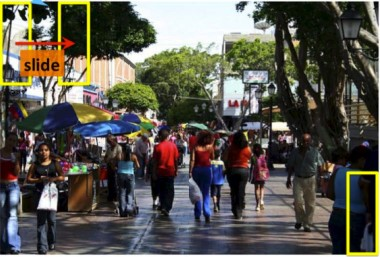
\includegraphics[scale = 1.5]{img/sliding window.jpg}
        \label{sliding_window}
        \caption{Sliding window}
\end{figure}

Moreover, in order for the \textit{pedestrian detector} to detect persons of very different scales in the same image, the window also scans a down-scaled version of the image, while the size of the window remains the same. This operation is repeated for many down-scaled version of the image, where the scale differences across the scans are small.

\subsubsection{Feature vector}
The second phase of the \textit{pedestrian recognition} solving method is given by the \textit{feature vector} creation. Since the method which is used for creating each feature vector is based on another family of methods, we first introduce the latter methods in order to better understand the former one.

\underline{Support Vector Machines (SVM)}
\\
One of the most important family of ML algorithm is represented by the \textbf{Support Vector Machines (SVM)}, which were introduced after the diffusion of the \textit{Backpropagation} algorithm, and which are very connected to \textit{Statistical Learning Theory}. \textit{SVM} deals with 
binary classification problems (with the assumption that the problem is linearly separable), and it belongs to the class of \textit{discriminative classifiers}, since its goal consists on learning the class boundary between the two classes $y$ starting from features $x$. More specifically, the goal of \textit{SVM} is to find, among all the possible class boundaries between the two classes, the one that is furthest from the two classes. If the distance between the closest points of two different classes is called \textbf{margin}, then \textit{SVM}'s goal is to separate the instances of the two classes with a boundary that \textbf{maximizes the margin}: intuitively, the farthest the boundary is from the points, the greater the confidence in the prediction is. Picture \ref{margin} provides a visual representation of the margin: the instances of the two classes that determine the margin, i.e. the red circled points, are called \textbf{support vectors}. In this sense, we can easily notice that decision boundary only depends on the support vectors, since they're the only points that determine the width of the margin. 

\begin{figure}[h!]
		\centering
		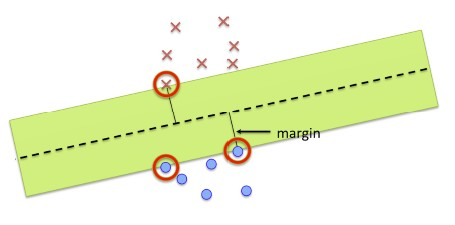
\includegraphics[scale = 1.5]{img/margin.jpg}
        \label{margin}
        \caption{Margin and support vectors}
\end{figure}

If we denote as $w^tx + b = 0$ (or, equivalently, as $c(w^tx + b) = 0$) the plane which separates the instances of the two classes, i.e. the decision boundary, then we can normalize the points of the dataset so that the \textit{positive} support vectors, i.e. the support vectors \textit{above} the decision boundary, lie on this plane:

$$
w^tx + b = +1
$$
, while the \textit{negative} support vectors on this one:

$$
w^tx + b = -1
$$

In this way, the distance between each support vector and the decision boundary is given by $\frac{1}{||w||}$, so the \textbf{equation of the margin} is $\frac{2}{||w||}$. A visual representation of these relationships is provided in Picture \ref{margin2}.

\begin{figure}[h!]
		\centering
		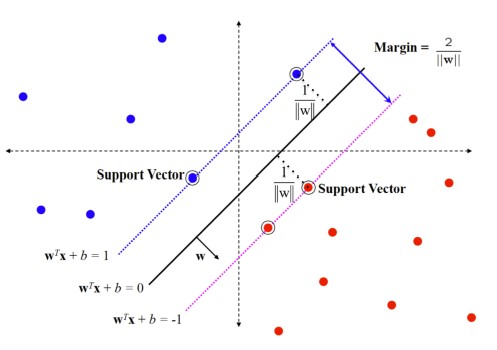
\includegraphics[scale = 1.7]{img/margin2.jpg}
        \label{margin2}
        \caption{Margin and support vectors}
\end{figure}

As we said before, the goal of \textit{SVM} is to maximize the margin, so learning the \textit{SVM} can be formulated as the following optimization problem:

\begin{equation}\label{svmopt}
\begin{aligned}
&\min_{w} \quad ||w||^2\\
&\text{s.t.} \quad y_i(w^Tx_i+b) \geq 1 \qquad i = 1,\dots, N\\
\end{aligned}
\end{equation}

The formulation of \ref{svmopt} represents an optimization problem on a convex function and with only linear constraints. Due to the nature of the problem we have a \textbf{unique minimum} solution which corresponds to the \textbf{optimal margin classifier}.

One of the issues of \textit{SVM} is to make decisions in presence of outliers.
\begin{figure}[h!]
		\centering
		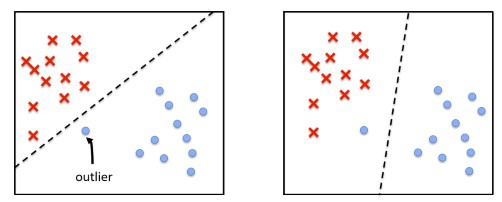
\includegraphics[scale = 1.7]{img/outliers.jpg}
        \caption{SVM in presence of outliers}
\end{figure}
The previous image shows the effect that a single outlier can have. We can make only one of the following choices: correctly classify the outlier, thus reducing the robustness of the classifier, or leave the outlier as misclassified. The strategy which is commonly adopted is the second one, as it provides more generalization to the classifier. In order to reduce the effects of mis-classification we introduce some \textbf{slack variables}, useful for allowing some errors in the boundary. More specifically, a slack variable is created for each example of the training set, and each slack variable indicates how much the constraints are violated. For example, Picture \ref{slack} shows an example of examples of the training set and the respective slack variables: in one case the value of the slack variable is 0.6, indicating that the training instance is violating the constraints of the boundary but it still classified correctly since the value is smaller than 1. In the second case, the value is 1.3, which means the instance is wrongly classified.

\begin{figure}[h!]
		\centering
		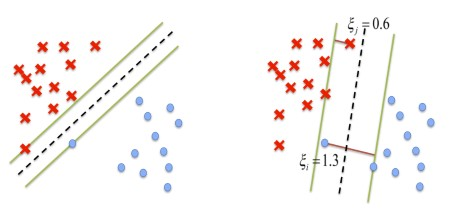
\includegraphics[scale = 1.7]{img/soft margin.jpg}
        \label{slack}
        \caption{Slack variable example}
\end{figure}

Now the optimization problem can be re-formulated as:
\begin{equation*}
\begin{aligned}
&\text{min} \quad \frac{1}{2}||w||^2+ C\sum\limits_{i = 1}^N\xi_i\\
&\text{s.t. } y_i(w^Tx_i-b)\geq 1 - \xi_i\\
&\xi_i \geq 0 \qquad i = 1,\dots,N
\end{aligned}
\end{equation*}

The only parameter C controls the \textbf{tradeoff} between the accuracy with respect to the training data and the maximization of the margin. It can be interpreted also as a \textbf{regularization term}:

\begin{itemize}
	\item small $C$ allows constraints to be easily ignored \textit{(large margin)}, allowing more misclassifications.
	\item large $C$ makes constraints hard to ignore \textit{(narrow margin)}, allowing less misclassifications.
	\item $C = \infty$ enforces all constraints \textit{(hard margin)}, so in this case no misclassification occurs.
\end{itemize}

\underline{Histograms of Oriented Gradients (HOG)}
\\

We can now focus on the method which was used to extract the feature vector from each window. The method is called \textbf{Histograms of Oriented Gradients (HOG)}, and it was introduced by \cite{dalal2005histograms}. As we said before, its goal is to create a robust feature set that allows the human form to be discriminated cleanly, even in cluttered backgrounds under difficult illumination. Picture \ref{hog} provides an overview of the feature extraction chain.

\begin{figure}[h!]
		\centering
		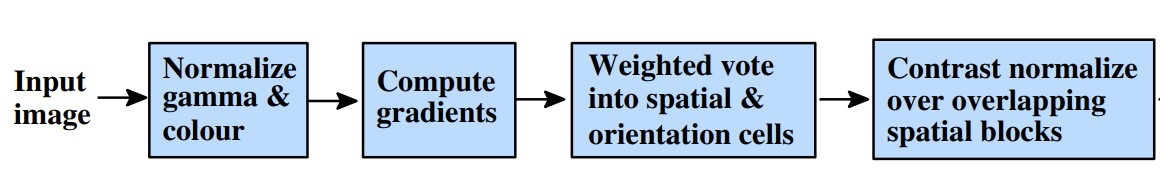
\includegraphics[scale = 1.2]{img/hog.jpg}
        \label{hog}
        \caption{Overview of HOG method}
\end{figure}

The basic idea is that local object appearance and shape can often be characterized rather well by the \textbf{distribution} of local intensity \textbf{gradients} or edge directions, even without precise knowledge of the corresponding gradient or edge positions. In this sense, we can notice that the method is based on the concept of gradient, and in particular on the distribution of gradients.

If we have a 1-variable function the gradient is computed as:

$$
\frac{df}{dx} = \lim_{\Delta x \to 0} \frac{f(x) - f(x - \Delta x)}{\Delta x} = f'(x) 
$$

Suppose that the function is discretized, i.e. it is obtained by sampling a continuous function, then the approximated gradient is given by:

$$
\frac{df}{dx} = \frac{f(x) - f(x - 1)}{1} = f(x) - f(x - 1) = f'(x) 
$$
, i.e. the approximated gradient is computed as the difference of two consecutive discrete points.

If we consider a 2-variables function, then the following relations hold:

\begin{figure}[h!]
		\centering
		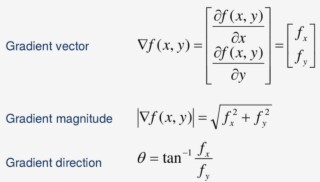
\includegraphics[scale = 1.6]{img/2dim.jpg}
\end{figure}

, so for computing each component $\frac{\delta f(x,y)}{\delta x}$ and $\frac{\delta f(x,y)}{\delta y}$ an approximation can be used. \textit{HOG} method uses the following computation:

$$
f'(x) = \lim_{h \to 0} \frac{f(x+h) - f(x-h)}{2h}
$$

Therefore, in this case if we have a point centered in $(0,0)$, then $\frac{\delta f(x,y)}{\delta x} = $ [-1, 0, 1], while $\frac{\delta f(x,y)}{\delta y} = $ \begin{bmatrix} -1 \\ 0\\ 1 \end{bmatrix}

As an example, the gradient of the pixel in Picture \ref{example} is given by $(94-56), (93-55)$, i.e. $(38, 38)^T$, while the angle is $arctan(\frac{38}{38}) = 45$ degrees.

\begin{figure}[h!]
		\centering
		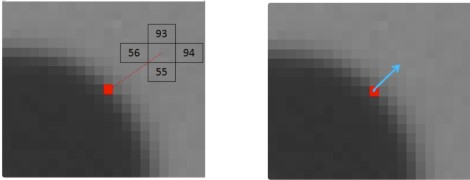
\includegraphics[scale = 1.6]{img/example.jpg}
          \label{example}
          \caption{Example of computation of the gradient and its direction}
\end{figure}

Using the gradient distribution, we can compute the gradient magnitude and direction, i.e. the angle, for each of the pixels in the image, as shown in Picture \ref{gradient_example}.

\begin{figure}[h!]
		\centering
		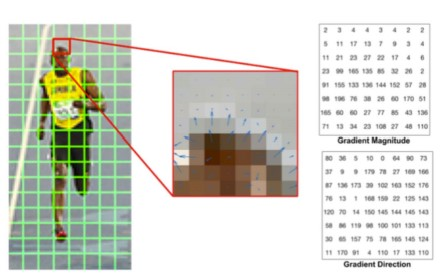
\includegraphics[scale = 2.0]{img/gradient_example.jpg}
          \label{gradient_example}
          \caption{Example of computation of the gradient and its direction for each pixel of the image}
\end{figure}

Once we introduced this method for gradient computation, we can now analyze how it is used for the task of feature extraction implemented by \textit{HOG}. This method follows these steps:

\begin{enumerate}
    \item Compute centered horizontal and vertical gradients with no smoothing;
    \item Compute gradient orientation and magnitudes (for color images, pick the color channel with the highest gradient magnitude for each pixel);
    \item Divide the 64x128 image into 16x16 blocks with 50\% of overlap (for a total of 7x15 = 105 blocks). Each block should consist of 4 cells with size 8x8, in which the gradient is computed. A visual representation of the blocks and the cells is provided in Picture \ref{cells_blocks}.

    \begin{figure}[h!]
		\centering
		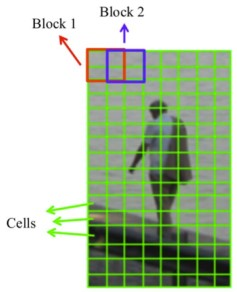
\includegraphics[scale = 2.0]{img/cells_blocks.jpg}
          \label{cells_blocks}
          \caption{Partition of the image into cells and blocks}
    \end{figure}

    \item For each 8x8 cell, compute the histogram of the gradient orientation binned into 9 bins: the vote of the cell is given by the gradient magnitude, and each vote is linearly interpolated between neighboring bin centers. For example, if the orientation is 85 degrees, then the distances to the bin center 70 and 90 are 15 and 5 degrees respectively. Hence, the vote is splitted into $\frac{5}{20} = 0.25$ for Bin 70, and $\frac{15}{20} = 0.75$ for Bin 90.

    \begin{figure}[h!]
		\centering
		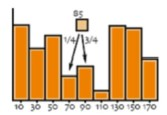
\includegraphics[scale = 2.0]{img/vote}
    \end{figure}

    Note that the vote could be also weighted with a Gaussian function in order to downweight the pixels near the edges of the block.

    \item Concatenate the 4 cell histograms in each block into a single block feature $f$ and normalize $f$ by its Euclidean norm, i.e.:

    $$
    f = \frac{f}{\sqrt{||f||_2^2 + \epsilon^2}}
    $$
    , where $\epsilon$ is used to have better performances.

    \item Finally, the final feature vector is composed of 3,780 histograms.
    
\end{enumerate}

\subsubsection{Classification phase} 
Once the feature extraction phase is done, the classification can be performed. This classification phase was composed by:

\begin{itemize}
    \item a \textbf{learning phase}, in which an SVM classifier was trained with the feature vectors resulted by the HOG method;
    \item a \textbf{test phase}, in which the classifier was asked to predict the presence or the absence of a person in each window in the image.
\end{itemize}

Since this new approach gave near-perfect separation on the original MIT pedestrian database (507 positive windows only training set, 200 positive windows only test set), the authors introduced a more challenging dataset containing over 1,800 annotated human images with a large range of pose variations and backgrounds. The training dataset was composed of 1,208 positive windows examples and 1,218 negative windows examples, generated using the \textit{Bootstrapping} technique, while the test set by 566 positive examples and 453 negative examples.

\subsubsection{Post-processing phase}
As we saw for Viola and Jones, the algorithm resulted in multiple responses around positive examples, so the \textit{non-maximum suppression} technique was performed, in order to remove all the boxes that overlapped more that 50\% with another box.

\begin{figure}[h!]
		\centering
		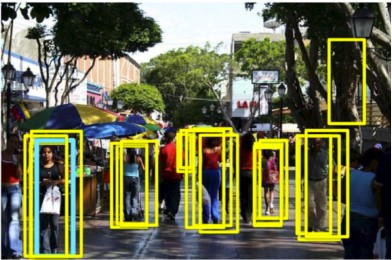
\includegraphics[scale = 2.0]{img/multiple boxes.jpg}
\end{figure}


\begin{figure}[h!]
		\centering
		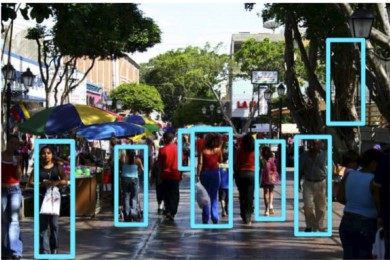
\includegraphics[scale = 2.0]{img/results.jpg}
\end{figure}

\section{Deep Neural Networks} \label{ch4}
The \textbf{philosophy} on which \textbf{Deep Learning} relies is to provide a new method for selecting and extracting the features that are provided as input to a classifier, by exploiting the data of the training set. 

More specifically, instead of selecting manually good features and then using them to feed a classifier, Deep Neural Networks learn from the data a \textbf{feature hierarchy} from the initial pixel image in order to obtain a \textbf{classifier}: each layer extracts features from the output of the previous layer, and finally the training phase involves all the layers, jointly.
\image{img/deep_learning}{Example of deep learning process.}{0.75}

As we can see, each layer of the pipeline learns to extract features from the image/video/pixels (in general, from the data we have), and the \textbf{deeper} the layer is, the \textbf{more abstract} the extracted features are.

\subsection{Shallow vs Deep Networks} \textbf{Shallow architectures} are \textbf{inefficient} at \textbf{representing deep functions}, since they are characterized by a limited number of hidden layers. A shallow network with a large single hidden layer can fit any function (i.e. it is a universal approximator), but on the other hand this increases significantly the number of parameters. 

A \textbf{deep network} can \textbf{fit} functions \textbf{better} with less parameters than a shallow network, increasing the number of hidden layers but decreasing the number of required parameters. Deep networks try to simulate the brain's behavior, in which the electric signals propagate across different layers.
\image{img/shallow_vs_deep}{Shallow vs Deep Networks.}{0.78}

Another important aspect to notice is the \textbf{improvement} in \textbf{performance} with the presence of more data.
\image{img/performances}{Performances improves with more data.}{0.6}
As we can see, in the case of basic ML algorithm after a certain amount of data the performance does not increase anymore: in SVM's, for example, this phenomenon happens since the decision boundary obtained by the model only depends on the support vectors, so increasing the size of the training set does not change the accuracy.

The \textbf{usage} of deep networks is not a \textbf{recent} idea (indeed, these networks are fairly old), but it has been made possible only nowadays thanks to the fact that we have \textbf{more data} and \textbf{more computing power}. In particular, the advances in the field of \textbf{GPUs} have made using deep networks way more feasible than before.

\paragraph{Image classification.} The \textbf{image classification} problem consists in predicting a single label (or a probability distribution over all the possible labels to indicate our confidence, as per the following example) for a given image. Images are 3-dimensional arrays of integers from 0 to 255 of size Width x Height x 3. The 3 represents the three color channels Red, Green and Blue.
\image{img/image_classification}{Image classification example.}{0.5}
In image classification, the most important \textbf{challenges} are the following ones:

\image{img/challenges}{Challenges in image classification.}{0.95}
In order to face these challenges, what we need is a data-driven approach in which we have thousands of categories and hundreds of thousand of images for each category.\\
As it is possible to understand, there's a difference between \textbf{traditional approaches} and \textbf{deep learning}. Indeed, in the first one we extract \textbf{meaningful features} from images through a \textbf{manual} process, while in the second case everything happens \textbf{automatically} thanks to a sequence of \textbf{layers} in which the final ones are useful for classification.

\paragraph{Inspiration from biology.} As we introduced before, functioning of Deep Neural Networks is highly inspired from biology, and in particular the architecture resembles the one in the visual cortex of the brain. Indeed, biological vision is hierarchically organized, and the basic component of this hierarchy is the \textbf{retina}. The cells of the retina are arrayed in discrete layers, with the \textbf{photoreceptors} at the top of them that are divided into:

\begin{itemize}
    \item \textbf{Rods}, which are sensitive to the intensity of the light and to movements;
    \item \textbf{Cones}, which are sensitive to colors.
\end{itemize}

We define \textbf{receptive field} the region of the visual field in which light stimuli evoke responses of a given neuron. In terms of Deep Networks, this makes a distinction between \textbf{fully connected Neural Networks}, in which each neuron is connected to all the neurons of the previous layer, and \textbf{sparsely connected Neural Networks}, in which each neuron is characterized by a corresponding \textbf{receptive field}, i.e. it is connected only to a subset of neurons of the previous layer.

The \textbf{take-home} message of this digression is that the \textbf{visual system} is a \textbf{hierarchy} of \textbf{features detectors}.

\paragraph{The Neocognitron (1980).} The first example example of self-trained network for feature learning was the \textbf{Neocognitron}, introduced in 1980.

\subsection{Convolution}
The \textbf{convolution} is a mathematical operation that takes as input an \textbf{image}, i.e. an array of pixels, and a 3x3 array of numbers (called \textbf{convolution filter}), and applies the 3x3 array in a certain portion of the image, and computes the summation of the products between the pixels of the image and the one in the filter. 

\begin{figure}[h!]
		\centering
        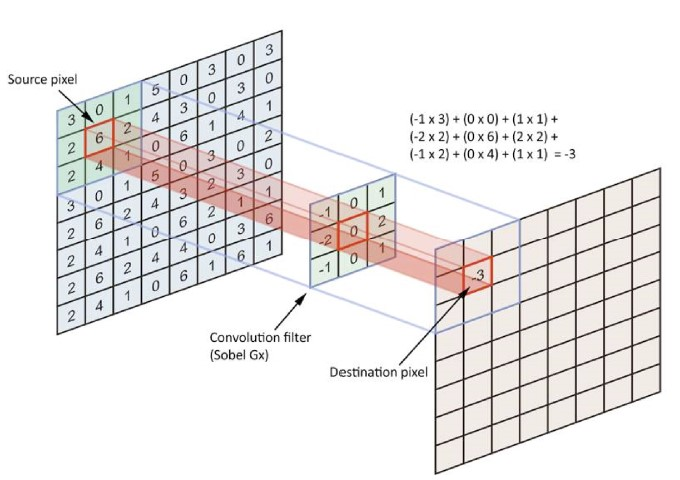
\includegraphics[scale = 1.5]{img/convolution.jpg}
		\label{mi}
        \caption{Example of convolution}
\end{figure}

Notice that there exist many type of filters, which differ for their values.

\begin{figure}[h!]
		\centering
        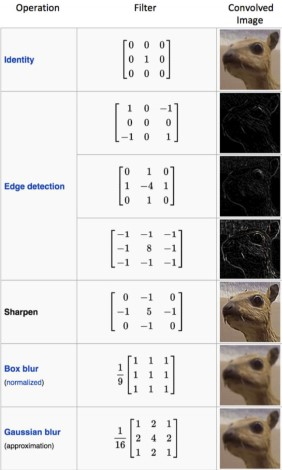
\includegraphics[scale = 1.5]{img/filters.jpg}
		\label{mi}
        \caption{Types of filters}
\end{figure}

\subsubsection{Stride and Padding}

The \textbf{stride} quantity denotes how many steps we're moving in each step of convolution, and the default value is 1. In order to maintain the dimension of the output the same as the one of the input, we use \textbf{padding}, which is the process of adding 0s to the input matrix symmetrically.

\begin{figure}[h!]
		\centering
        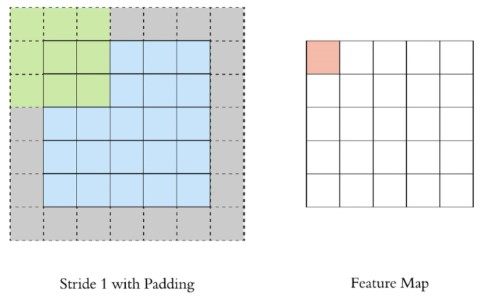
\includegraphics[scale = 1.5]{img/stride and padding.jpg}
		\label{mi}
        \caption{Stride $= 1$ with padding $ = 1$}
\end{figure}

In this sense, \textbf{stride} and \textbf{padding} can be used to \textbf{adjust} the \textbf{dimensionality} of the \textbf{data} effectively.

\subsubsection{Multiple channels}

In the case in which the convolution is applied to an image with multiple channels, we can use a different filter for each channel, and then combine the results into a single output matrix.

\begin{figure}[h!]
		\centering
        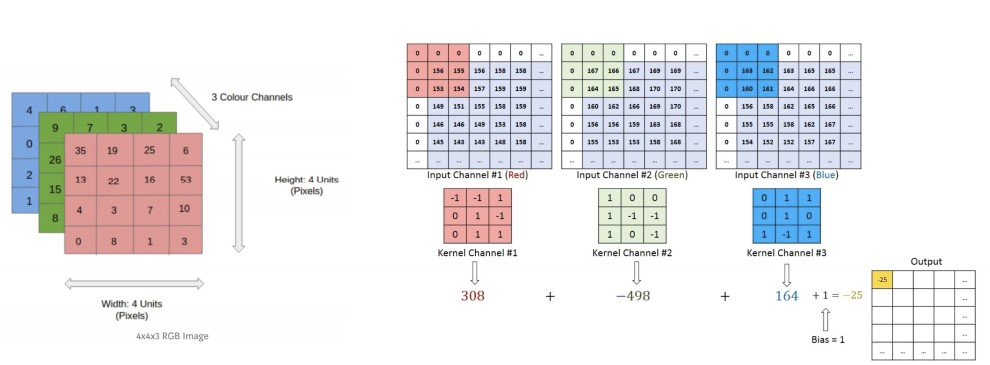
\includegraphics[scale = 1.5]{img/convolution with multiple channes.jpg}
		\label{mi}
        \caption{Example of convolution of an image with multiple channels}
\end{figure}

\subsubsection{Gaussian filter}

A very famous filter used in convolution is the Gaussian filter, which basically computes a weighted average of the pixels of the image, where the weights are proportional to the distance with the central pixel.

\begin{figure}[h!]
		\centering
        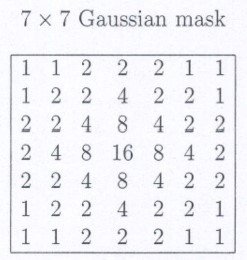
\includegraphics[scale = 1.5]{img/gaussian filter.jpg}
		\label{mi}
        \caption{Example of 7x7 Gaussian filter}
\end{figure}

The result of applying a Gaussian filter to an image is to obtain a \textbf{blurred version} of the image: the larger the filter, the more blurred the output image is.

\subsubsection{Convolution for edge detection and other problems}
An important application of the convolution operation is \textbf{edge detection}, i.e. the problem of determining the contour of an object.

\begin{figure}[h!]
		\centering
        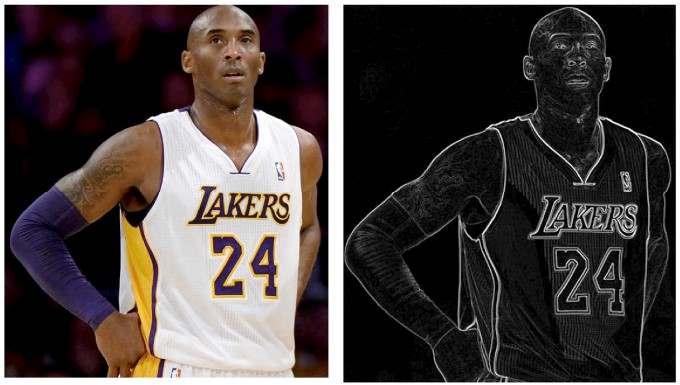
\includegraphics[scale = 1.5]{img/edge detection.jpg}
		\label{mi}
        \caption{Edge detection problem}
\end{figure}

Some of the most famous filters that are used in edge detection are \textit{Roberts operator}, \textit{Sobel operator} and \textit{Prewitt operator}. Other filters are used for different tasks, e.g. \textit{HoG} is used for the problem of \textit{pedestrian recognition} etc..

\subsection{Convolutional Neural Networks (CNNs)} 
\subsubsection{Fully-connected and sparsely-connected networks}
A neural network can be defined as a \textbf{fully-connected network} or a \textbf{locally-connected network}. In a fully-connected network, each neuron of each layer is connected to every neuron in the previous one, and each connection has its own weight. In this sense, the number of parameters is huge.

Conversely, in a locally-connected layer, each neuron is only connected to a \textbf{few nearby neurons} in the previous layer, and the same set of weights (and local connection layout) is used for each neuron. The typical use case for locally-connected layers is for image data where, as required, the \textbf{features} are \textbf{local} (e.g. a "nose" consists of a set of nearby pixels, which are not spread across the whole image), or in general in applications where the local connections capture local dependencies. The smaller number of connections and weights makes local-connected layers \textbf{relatively cheap} in terms of memory and computing power needed.
\image{img/fully_local}{Fully vs local-connected networks.}{0.75}

\subsubsection{Weight sharing}

Before providing the definition of \textbf{CNN}, we now define the concept of \textbf{weight sharing}. This concept is based on the following reasonable assumption: if one feature is useful to compute at some spatial position $(x_1, y_1)$, then it should be useful to compute at a different position $(x_2, y_2)$. In this way we can dramatically reduce the number of parameters.

\begin{figure}[h!]
		\centering
        \includegraphics[scale = 1.5]{img/weight sharing.jpg}
		\label{mi}
        \caption{Edge detection problem}
\end{figure}

As we can see, in the first case we have neurons detecting different features (i.e. different weights in the receptive fields), while in the second case the two neurons have the same weights in the corresponding receptive fields, so they're detecting the presence of the same feature in different portions of the image. Note that while in the traditional convolution operation the weights are applied directly to the pixels of the image, in this case they become the weights of the connections of the receptive fields. 

\subsubsection{Definition of CNN}
A \textbf{Convolutional Neural Network (CNN)} is a \textbf{multi-layer feed-forward neural network} characterized by \textbf{local connectivity} (i.e. neurons with the correspondent receptive field) and \textbf{weights} that are \textbf{shared} across spatial positions. Normally, \textbf{several filters} are \textbf{packed} together and \textbf{learned automatically} during training.
\image{img/trainableFilters}{Using Several Trainable Filters.}{0.75}

\paragraph{Pooling.}\textbf{Pooling} is a way to \textbf{simplify} the network architecture, by downsampling the \textbf{number of neurons} resulting from the filtering operations. An example of pooling technique is the \textbf{max pooling}, in which the \textbf{image} is \textbf{partitioned} in small squares and for each square the pixel with \textbf{maximum value} is taken.
\image{img/max_pooling}{Max Pooling.}{0.6}
As we can see in the next image, a \textbf{Deep Convolutional Neural Network} is a \textbf{combination} of \textbf{feature extraction} and \textbf{classification processes}:

\begin{itemize}
    \item The \textbf{input} of the network is represented by an \textbf{image};
    \item The \textbf{input layer} is followed by some \textbf{locally-connected layers} that \textbf{extract features} from the image. As we can see, this feature extraction phase is mainly composed of \textit{convolution} and \textit{subsampling} operations;
    \item Finally, a \textbf{fully-connected layer} provides the \textbf{classification} of the input image.
\end{itemize}

\image{img/extraction_and_classification}{Combining Feature Extraction and Classification.}{0.7}

\subsection{AlexNet (2012)} 
The first example of Deep Convolutional Neural Network we examine is the \textbf{AlexNet}. This architecture was developed in 2012 for solving the problem of \textbf{image classification}, and it was trained using the \textit{ImageNet} dataset, comprising 1,000 categories, 1.2M training images and 150k test images. The results were astonishing, since the error was reduced by 22\% in only 3 years.

More specifically, this architecture is not so different from the one of the \textit{Neocognitron}, or from the one proposed by LeCun in 1998, but this was much larger. AlexNet is composed of \textbf{8 layers} as per the following schema:
\imageb{img/alexNetLayers}{0.18}
The first thing we can notice are that:

\begin{itemize}
    \item The \textbf{input} is given by an \textbf{image};
    \item The \textbf{first 5 layers} are used for \textbf{extracting features} for the classification phase: as we can see, we have a combinations of \textit{convolution} and \textit{pooling} operations;
    \item \textbf{Layer 6 and 7} provide the \textbf{classification} of the input: as we can see, in this case we exploit fully connected layers;
    \item The \textbf{output layer} is represented by a \textbf{Softmax} function, which provides a probability distribution of the classes of the input image.
\end{itemize}

\image{img/alexNet}{AlexNet architecture.}{0.8}

Diving deeper into these layers' characteristics, we can notice that:
\begin{itemize}
	\item \textbf{1st layer:} we have 96 kernels of size $(11 \times 11 \times 3)$, which are applied to the input image: the results is then convolved (stride = 4) and pooled. Notice that the output of the first layer has not a width of 96, and this is because it was splitted into two different outputs, each with width equal to 48. By looking at the top-9 patches for one filter we can observe that the neurons are very sensitive for colors and geometric forms, so they're very simple;
	\item \textbf{2nd layer:} we have 256 kernels of size $(5 \times 5 \times 48)$, which are then normalized and pooled. Notice the 256 kernels are given by two blocks of 128 kernels. Here the neurons distinguish more abstract features, and this process continues as we go deeper in the Deep Network;
	\item \textbf{3rd layer:} we have 384 kernels of size $(3 \times 3 \times 256)$;
	\item \textbf{4th layer:} we have 384 kernels of size $(3 \times 3 \times 192)$;
	\item \textbf{5th layer:} we have 256 kernels of size $(3 \times 3 \times 192)$;
	\item \textbf{6th layer:} we have a fully connected layer with 4096 neurons;
	\item \textbf{7th layer:} we have a fully connected layer with 4096 neurons;
	\item \textbf{8th layer:} we have a 1000-way \textbf{SoftMax} output layer, i.e. 1 output for each of the possible classes, since it provides a probability distribution.
\end{itemize}
While training the network, two independent GPUs run in parallel, in order to speedup the training process. This is the reason why the output of the first layer was splitted. 

The last \textit{SoftMax} layer gives as output:
$$y_i = \frac{e^{z_i}}{\sum_j e^{z_j}}$$
, where $z_i$ represents the output of the network and it is defined as:

$$
z_i = w_i^T \cdot x
$$

\begin{figure}[h!]
		\centering
        \includegraphics[scale = 1.5]{img/softmax.jpg}
		\label{mi}
        \caption{Output of the SoftMax function}
\end{figure}

Since the output of the SoftMax is a probability distribution over all the possible classes of the training set, we can compute the \textbf{Cross-entropy loss} between the actual output and the desired one, in order to measure the quality of the model.

\subsection{ReLU} \textbf{ReLU} is an acronym that stands for \textit{Rectified Linear Unit}. ReLUs are used to solve the \textbf{problem} that \textbf{sigmoid activation} takes only values in $(0,1)$. While propagating the gradient back to the initial layers, it tends to get closer and closer to $0$ (this phenomenon is called \textit{vanishing gradient}, and it intensifies when the number of layers is high). From a practical perspective, this slows down the training procedure of the initial layers of the network. Indeed, with sigmoid the gradient will be close to 0 and the algorithm won't learn. In order to speed up the learning phase, ReLU is used.
\image{img/relu}{Comparison between sigmoid and ReLU functions.}{0.8}
It is also possible to notice that ReLU reaches the \textbf{same results as sigmoid}, but \textbf{much faster}. In the following image, the solid line represents the convergence of a 4 layer CNN with ReLUs, while the dashed line represents an equivalent network with $tanh$ neurons. It can be noticed that the CNN with \textbf{ReLUs converges six times faster}.
\image{img/relu2}{Convergence of ReLU neurons.}{0.4}

\subsection{Mini-batch Stochastic Gradient Descent} 
We recall that in the back-propagation algorithm we can have either the \textbf{on-line} implementation or the \textbf{off-line} one: in the first one, the weights are updated at any presentation of an example of the training set, while in the second one the gradient is computed exactly. We indicated the \textbf{stochastic gradient descent} as a possible compromise between the two approaches, now we introduce the \textbf{mini-batch stochastic gradient descent}, which is defined as follows:

\begin{enumerate}
	\item Sample a batch of data (the dimension is an hyperparameter to choose), i.e. a subset of the training set;
	\item Perform the forward pass and compute the loss;
	\item Perform the backward pass to compute the gradients;
	\item Update the weights using the gradient (by minimizing the loss).
\end{enumerate} 

Notice that, like in stochastic gradient descent, the use of random samples helps in finding global minima.

\subsection{Data augmentation}
The easiest and most common method to \textbf{reduce overfitting} on image data is to \textbf{artificially enlarge} the \textbf{dataset} using \textbf{label-preserving transformations}. This technique is used to make the dataset more robust. \textbf{AlexNet} uses two forms of \textbf{data augmentation}:
\begin{itemize}
	\item The first form consists in \textbf{generating image translations} and \textbf{horizontal reflections} (translations, scaling or rotations of the images);
	\item The second form consists in \textbf{altering the intensities} of the \textbf{RGB channels} of the \textbf{training images} (introduce random noise inside the images). 
\end{itemize}

\image{img/dataAugmentationBoys}{Data augmentation: translation, reflection, scaling, rotation, RGB noise.}{0.35}

\subsection{Dropout} This technique is exploited in order to have a network with \textbf{more generalization power}, and it consists on \textbf{randomly dropping out some neurons} during the back-propagation algorithm, by setting to 0 the output of that neuron with probability $0.5$. The neurons which are \textit{"dropped out"} in this way do not contribute to the forward pass and do not participate in back-propagation. Every time an input is presented, the neural network samples a different architecture, but all these architectures share weights.\\
Dropout reduces complex co-adaptations of neurons, and it forces the network to find different "roads" in order to produce the outputs, resulting in a more robust network.
\image{img/dropout}{Dropout results}{0.55}

\subsection{Feature analysis}
A well trained Deep Convolutional Neural Network is an excellent \textbf{feature extractor}: in particular, the idea is to chop the network at a desired layer and use the output as a feature representation to train a SVM on some other dataset. Here we show some results.

\begin{figure}[h!]
		\centering
        \includegraphics[scale = 2.0]{img/feature extraction.jpg}
		\label{mi}
        \caption{Results using CNN's as feature extractors}
\end{figure}

The parenthesis indicates the layer at which the output is taken: as we can see, the accuracy of the classifier increases as we choose features from more layers, underlying the property of CNN's of learning more and more accurate features as the number of layers grow.

\subsection{CNN's in computer vision tasks}
After 2012, many CV tasks were addressed using CNN's, for example:

\begin{itemize}
    \item \textbf{Semantic segmentation}: in this case the input is an image, and each pixel is classified with a label. An application of this kind of problem can be found in the autonomous driving systems and in medical image diagnostics;
    \item \textbf{Classification and localization}: in this case we assume that the input image contains a single prominent object, and the output consists of single label of the object (standard classification) together with the position of the object;
    \item \textbf{Object detection}: in this case we detect all the objects in an image, where the number is not known in advance;
    \item \textbf{Instance segmentation}: this problem represents a variation of the image segmentation problem, and it consists of labeling each pixel differentiating between objects having the same label.
\end{itemize}

\begin{figure}[h!]
		\centering
        \includegraphics[scale = 1.5]{img/cv tasks.jpg}
		\label{mi}
        \caption{Computer vision problems}
\end{figure}

In general, the adoption of CNN's for solving such problems is having a huge impact in the results.

\subsubsection{Semantic segmentation}
As we introduced before, the goal of semantic segmentation is to assign a semantic label to each and every pixel of the image, and we can take into consideration two important features:

\begin{itemize}
    \item The contextual information is quite useful in this problem;
    \item We cannot exploit the architecture of AlexNet for solving this problem, since AlexNet provides a probability distribution. However, we can exploit the part of the network responsible for the feature extraction phase.
\end{itemize}

\paragraph{First idea: sliding window}
\\
The first method for solving this problem is represented by the \textbf{sliding window} approach: in this case a small \textbf{patch} is moved along the image, and each \textbf{center pixel} of the patch is \textbf{classified} using a \textbf{CNN}. 

\begin{figure}[h!]
		\centering
        \includegraphics[scale = 2.0]{img/semantic1.jpg}
		\label{semantic1}
        \caption{Sliding window for semantic segmentation}
\end{figure}

Clearly, this approach suffers from different problems:

\begin{itemize}
    \item First of all, it is very \textbf{inefficient};
    \item Secondly, it does not exploit the contextual information, i.e. shared features between overlapping patches are not reused.
\end{itemize}

\paragraph{Second idea: fully convolutional}
\\
In this case the idea is to exploit the feature extractor part of the AlexNet architecture, in order to use the features to produce the output of each pixel. 

\begin{figure}[h!]
		\centering
        \includegraphics[scale = 2.0]{img/semantic2.jpg}
		\label{semantic2}
        \caption{Fully convolutional NN for semantic segmentation}
\end{figure}

As we can see from the image, the network is composed by several \textbf{convolutional layers} that are applied to the \textbf{input image}, and the result is, for each pixel, a vector of elements representing a \textbf{probability distribution}. Despite being \textbf{more efficient} than the previous method (in this case we can compute the predictions for the pixels all at once), this method suffers from a \textbf{problem}: since we do not use \textbf{pooling}, convolutions at original image resolution will be very \textbf{expensive}. For this reason, we can consider a variation of this method, which exploits the \textbf{encoder-decoder} architecture.

\paragraph{Third idea: fully convolutional with downsampling and upsampling}
\\

\begin{figure}[h!]
		\centering
        \includegraphics[scale = 2.0]{img/semantic3.jpg}
		\label{semantic2}
        \caption{Fully convolutional NN for semantic segmentation with encoder-decoder}
\end{figure}

As we can see, the network is composed by several \textbf{convolutional layers} that are applied to the \textbf{input image}, with the difference that in this case \textbf{downsampling} and \textbf{upsampling} are contained in the network. The downsampling allows to encode the image into a feature map whose dimensionality is lower than the original image, while the upsampling takes as input the output of the downsampling phase, and it produces as output an image with the same size of the original one. The downsampling phase is performed by the \textbf{encoder}, while the upsampling is performed by the \textbf{decoder}. While for the downsampling phase, an idea could be to exploit the convolutional layers of AlexNet or any other CNN, for the upsampling phase (also called unpooling) the reasoning is not as simple.

\textbf{In-network upsampling}
Picture \ref{unpooling} shows some possible implementations of the unpooling phase:

\begin{itemize}
    \item \textit{Nearest neighbor}, i.e. the new entries are filled with the same value of the original patch;
    \item \textit{"Bed of nails"}, i.e. the new entries are filled with 0s;
    \item \textit{Max unpooling}, i.e. the new entries are filled in the positions corresponding to the maximum elements in the Max pooling layer.
\end{itemize}

\begin{figure}[h!]
		\centering
        \includegraphics[scale = 1.0]{img/unpooling1.jpg}
        \includegraphics[scale = 1.0]{img/unpooling2.jpg}
		\label{unpooling}
        \caption{Fully convolutional NN for semantic segmentation with encoder-decoder}
\end{figure}

Moreover, we can exploit the same reasoning of pooling to perform the upsampling, in order to obtain the so-called \textbf{transpose convolution}, represented in Picture \ref{transpose convolution}.

\begin{figure}[h!]
		\centering
        \includegraphics[scale = 1.0]{img/transpose_convolution3.jpg}
        \includegraphics[scale = 0.3]{img/transpose_convolution4.jpg}
		\label{transpose convolution}
        \caption{Transpose convolution}
\end{figure}

However, in 2015 it was discovered that the pipeline did now work well, in particular in solving both the WHAT and WHERE problem:

\begin{itemize}
    \item The \textit{what} problem refers to the problem of classifying the prominent object;
    \item The \textit{where} problem refers to the problem of locating where the object is.
\end{itemize}

\begin{figure}[h!]
		\centering
        \includegraphics[scale = 0.35]{img/transpose_convolution5.jpg}
		\label{transpose convolution}
        \caption{Transpose convolution}
\end{figure}

If we consider the above Picture, we notice that after layer 7, we extracted powerful features for the WHAT problem, but at the same time we lost some information about the location, i.e. the WHERE problem. In this sense, the idea is to consider an architecture with \textbf{branches}, which allow to skip some layers and results in having better performances for the WHERE problem. Picture \ref{skip layers} compares the results obtained by the original CNN and the ones exploiting the techinque we just described.

\begin{figure}[h!]
		\centering
        \includegraphics[scale = 0.3]{img/semantic4.jpg}
        \includegraphics[scale = 0.3]{img/semantic5.jpg}
		\label{skip layers}
        \caption{CNN with skipping layers technique}
\end{figure}

\paragraph{U-net}
The architecture of the U-net is very similar to the one showed in \ref{skip layers}, with the difference that in this case the network is implemented for medical diagnosis. 

\begin{figure}[h!]
		\centering
        \includegraphics[scale = 0.3]{img/unet.jpg}
		\label{unet}
        \caption{U-net}
\end{figure}

The evaluation of the network is splitted into:

\begin{itemize}
    \item A \textit{contraction phase}, which reduces the spatial dimensions, thus increasing the WHAT;
    \item An \textit{expansion phase}, which recovers object details and dimensions, thus increasing the WHERE.
\end{itemize}

\subsubsection{Object detection}
The problem of \textbf{object detection} consists of \textbf{locating} and \textbf{classifying} the object(s) that are represented in an image. In this case we make the following assumptions:

\begin{itemize}
    \item The image containing a \textbf{single prominent object};
    \item The object is not rotated, i.e. it is \textbf{vertically oriented}.
\end{itemize}

The idea for solving this problem is the following: we exploit AlexNet (excluding the output layer) to obtain the features of the input image, and then we create two branches:

\begin{enumerate}
    \item The first one is responsible for solving the \textbf{classification} problem;
    \item The second one is responsible for solving the \textbf{regression} problem, i.e. of predicting the coordinates of the bounding box for the prominent object.
\end{enumerate}

The architecture of the network is represented in \ref{object detection 2}.

\begin{figure}[h!]
		\centering
        \includegraphics[scale = 0.35]{img/object detection2.jpeg}
		\label{object detection 2}
        \caption{Architecture of the network for solving the object detection problem}
\end{figure}

As we can see, the two branches are characterized by \textbf{two different losses}: the \textbf{softmax} is used for the classification branch (each label is characterized by a probability), while the \textbf{L2} is used for the regression one. For this reason, the idea is to combine the two losses into a new one, called \textbf{multitask loss}, which will be then considered by the backpropagation algorithm for updating the weights of the network.

Now, what can we do when there are more than 1 prominent object represented in an image? The intuition is to create a \textbf{new branch} for \textbf{each} of the \textbf{object}, but clearly this number is not known in advance, and for this reason a new approach must be considered. In this case the idea is to exploit a \textbf{sliding window} approach, i.e. to apply a CNN to many different crops of the image, in order to classify each crop as object or background.

\begin{figure}[h!]
		\centering
        \includegraphics[scale = 0.35]{img/object detection3.jpeg}
		\label{object detection 3}
        \caption{Object detection problem with sliding window approach}
\end{figure}

Clearly, the \textbf{downside} of this approach is that we need to apply a CNN to a huge number of locations, scales and aspect ratios, which results in having a very computationally expensive operation!

Another idea is to consider the so-called \textbf{region proposals}: we find some image regions that are likely to contain objects, and we run the classifier only over that regions. In this way the computation time becomes much lower (e.g. SelectiveSearch gives 2,00 region proposals in a few seconds on CPU).

\paragraph{R-CNN}

The \textbf{R-CNN} is a special CNN which is exploited for solving the object detection (with multiple objects) problem. The architecture is showed in Picture \ref{r-cnn}.

\begin{figure}[h!]
		\centering
        \includegraphics[scale = 0.50]{img/r-cnn.jpg}
		\label{r-cnn}
        \caption{Architecture of R-CNN}
\end{figure}

Some notes:

\begin{itemize}
    \item The \textbf{input} is represented by an image;
    \item A proposal method is exploited for finding the regions of interest (RoI, about 2,000) of the image;
    \item Since each of the RoI may be of different size, they're warped into regions of the same size;
    \item Each of the warped regions is provided as input to a CNN (excluded of the classification layer), in order to extract the features;
    \item The output of each of the CNN is provided as input to two different models:
    \begin{itemize}
        \item An SVM for classifying the region;
        \item A regression model for estimating the position of the bounding box.
    \end{itemize}
\end{itemize}

Among the \textbf{weaknesses} of this model, we have that:

\begin{itemize}
    \item The architecture is characterized by a lot of \textbf{loss functions}: a loss for the network (\textit{log loss}), a loss for the linear SVM (\textit{hinge loss}) and a loss for the regression model (\textit{least squares});
    \item The training phase is extremely slow (84h), and it takes a lot of disk space;
    \item The detection phase is slow too (47s per image with VGG16);
\end{itemize}

Notice that both the training and detection time are affected by the fact that a CNN is used for each of the RoI (about 2,000 CNNs).

\paragraph{Fast R-CNN}
Due to the weaknesses described above, in the following year (2015) a variation of R-CNN was developed, called \textbf{Fast R-CNN}, whose architecture is represented in \ref{fast r-cnn}.

\begin{figure}[h!]
		\centering
        \includegraphics[scale = 0.70]{img/fast r-cnn.jpg}
		\label{fast r-cnn}
        \caption{Architecture of Fast R-CNN}
\end{figure}

Some notes:

\begin{itemize}
    \item The network takes as \textbf{input} an \textbf{entire image} and a set of object proposals;
    \item The networks first processes the whole image with several \textbf{convolutional} and \textbf{max pooling} layers to produce a convolutional \textbf{feature map};
    \item For each object proposal, a \textbf{RoI pooling layer} extracts a fixed-length \textbf{feature vector} from the feature map;
    \item Each feature vector is fed into a sequence of \textbf{fully connected layers} that finally branch into \textbf{two} sibling \textbf{output layers}:

    \begin{itemize}
        \item One that produces a \textbf{SoftMax} probability estimates over $k$ object classes plus a catch-all \textit{background} class;
        \item Another layer that outputs 4 \textbf{real-valued numbers} for each of the $k$ object classes.
    \end{itemize}
    \item The two losses (\textit{log loss} and \textit{smooth L1 loss}) are combined into a \textit{multi-task loss}, which is then used in the backpropagation algorithm for updating the weights of the network.
\end{itemize}

Picture \ref{r-cnn vs fast r-cnn} provides a comparison between the training and testing time of R-CNN and Fast R-CNN: as we can see, \textbf{Fast R-CNN} is \textbf{faster} in both training and testing. Moreover, we can notice how Fast R-CNN is characterized by a fully trainable pipeline.

\begin{figure}[h!]
		\centering
        \includegraphics[scale = 0.70]{img/r-cnn vs fast r-cnn.jpg}
		\label{r-cnn vs fast r-cnn}
        \caption{Training and testing time comparison}
\end{figure}

However, if we consider the \textbf{testing time} of Fast R-CNN we notice how it is dominated by the algorithm for searching the region proposal (about 2s on a total of 2.3 s).

\paragraph{Faster R-CNN}
The last version of the model was proposed in 2016, and in this case the idea is to insert a Region Proposal Network (RPN) in order to predict the proposals from the features extracted by the CNN.

\begin{figure}[h!]
		\centering
        \includegraphics[scale = 0.70]{img/faster r-cnn.jpg}
		\label{faster r-cnn}
        \caption{Architecture of Faster R-CNN}
\end{figure}

In this case, the network is jointly trained with 4 losses:

\begin{itemize}
    \item The RPN loss for classifying object/non-object;
    \item The RPN loss for predicting the box coordinates;
    \item The final classification loss;
    \item The final bounding box regression loss.
\end{itemize}

As we can see from Picture \ref{faster r-cnn2}, Faster R-CNN represents the model with the lowest test-time, with the peculiarity of not being affected by the time of providing the proposals.

\begin{figure}[h!]
		\centering
        \includegraphics[scale = 0.40]{img/faster r-cnn2.jpg}
		\label{faster r-cnn2}
        \caption{Running times comparison}
\end{figure}

Finally, notice that also Faster R-CNN represents a fully trainable pipeline.

In general, the arrival of \textbf{Deep Learning} in 2012, the performances of object detection algorithms, together with other algorithms for other problems (e.g. speech recognition, NLP etc..) increased significantly.

\subsubsection{Human pose estimation}
This problem is an instance of the previous one, since the goal is to \textbf{detect humans}, but in this case using the \textbf{relative positions} of the parts of their \textbf{bodies}. Again, the assumption is that the image contains a single prominent human body.

The idea for solving this problem is to represent a \textbf{human pose} as a set of 14 joint positions, in order to represent a body with a tree. An example of these positions is given in Picture \ref{human pose 1}.

\begin{figure}[h!]
		\centering
        \includegraphics[scale = 0.35]{img/human pose estimation 1.jpg}
		\label{human pose 1}
        \caption{Representation of the joint positions}
\end{figure}

Now, the intuition is to consider once again the convolutional layers of AlexNet, and to create a branch for each of the 14 positions: each of the networks will then solve a regression problem for estimating the position of each of the parts of the human body. The architecture is showed in \ref{human pose 2}.

\begin{figure}[h!]
		\centering
        \includegraphics[scale = 0.45]{img/human pose estimation 2.jpg}
		\label{human pose 2}
        \caption{Architecture of the network for solving the human pose estimation problem}
\end{figure}

As in the previous problem, we have a loss for each of the branches (in this case the same loss, L2), which are eventually combined into a unique loss.

\subsubsection{Image captioning}
If we consider the problem of \textbf{image captioning}, i.e. of providing a textual description of the content of an image, it is clear that the usage of a \textbf{feed-forward neural network} does not help in this case, since the output depends on the input. For this reason, we have to exploit \textbf{recurrent neural networks}.

\begin{figure}[h!]
		\centering
        \includegraphics[scale = 0.8]{img/rnn1.jpg}
		\label{mi}
        \caption{Recurrent neural networks}
\end{figure}

The image shows the unfolding of the simplest recurrent NN, i.e. the one composed of a single hidden layer. Notice that this architecture is different from a feed-forward NN for two main reasons:

\begin{itemize}
    \item We do not know in advance the number of layers;
    \item In a feed-forward NN we have different weights between the layers, while in this case we only have 1 batch of weights for each connection.
\end{itemize}

If we denote with $W_{xh}$ the weights between the input vector $x$ and the RNN, with $W_{hh}$ the weights of the RNN and with $W_{hy}$ the weights between the RNN and the output vector, then:

$$
h_t = \text{tanh} (W_{hh} h_{t-1} + W_{xh} x_t)
$$

and 

$$
y_t = W_{hy} h_t
$$
, where $h_t$ represents the output of the hidden layer at time $t$.

We can have many types of RNN, as shown in the following image.

\begin{figure}[h!]
		\centering
        \includegraphics[scale = 0.8]{img/rnn2.jpg}
		\label{mi}
        \caption{Recurrent neural networks}
\end{figure}

\begin{itemize}
    \item The \textbf{one-to-many} RNN is used for solving the \textbf{image captioning} problem;
    \item The \textbf{many-to-one} RNN is used for solving the \textbf{sentiment classification} problem (i.e., given a sequence of words, provide the sentiment);
    \item The \textbf{many-to-many} RNN is used for solving the \textbf{machine translation} problem (i.e., given a sequence of words, translating it into another sequence of words). The many-to-many is also used for \textbf{video classification}.
\end{itemize}

\paragraph{Image captioning}
We focus now on the image captioning problem: the idea here is to exploit a CNN (in this case AlexNet) to extract the features of an image, and then use these features for training a RNN which can solve the problem.

$$
\text{Image} \to \text{CNN} \to \text{RNN}
$$

\begin{figure}[h!]
		\centering
        \includegraphics[scale = 1.5]{img/image captioning 1.jpg}
		\label{mi}
        \caption{Image captioning: training}
\end{figure}

As we can see, the last two layers are deleted, since we do not care about the actual classification of the image, but only on the feature the CNN extracted. Finally, the features are provided as input to the RNN, which returns the caption of the image. 

\begin{figure}[h!]
		\centering
        \includegraphics[scale = 1.5]{img/image captioning 2.jpg}
		\label{mi}
        \caption{Image captioning: test}
\end{figure}

At test time, an image without caption is provided as input to the CNN, the features are extracted, and then the RNN is used to provide the caption of the image.

\section{Dominant-set clustering}\label{ch5} 
We now focus on \textbf{unsupervised learning} problems, i.e. \textbf{clustering}, and in particular we focus on the \textbf{dominant set} approach for solving such problems.

\subsection{Graph-theoretic definition of a cluster}
These notes are based on \cite{pavan2006dominant}.

Data to be clustered are represented as an undirected weighted graph with no self-loops: $G=(V, E, \omega)$, where $V=\{1,\dots,n\}$ is the vertex set, $E\subseteq V\times V$ is the edges set and $w: E\rightarrow \mathbb{R}^*_+$ is the positive weight function. Vertices represent data points, edges neighborhood relationships and edge-weights similarity relations. $G$ is then represented with an adjacency matrix $A$, such that $a_{ij} = \omega(i,j)$. Since there are not self-loops we have that $\omega(i,i) = 0$ (main diagonal equal to $0$). From now on, if not otherwise stated, $A$ will represent such matrix. \\
There is \textbf{not} an \textbf{unique} and well defined \textbf{definition} of \textbf{cluster}, but the available literature agrees in two conditions that a cluster should satisfy:
\begin{itemize}
  \item \textbf{High internal homogeneity}, also named \textit{internal criterion}. It means that all the objects inside a cluster should be highly similar to (or have low distance from) each other;
  \item \textbf{High external inhomogeneity}, also named \textit{external criterion}. It means that objects coming from different clusters have low similarity (or high distance).
\end{itemize}
The idea of these criterion is that \textbf{clusters} are groups of objects which are \textbf{strongly similar} to each other if they belong to the same cluster, otherwise they are \textbf{highly dissimilar}. 

\paragraph{Basic definitions.}

Let $S\subseteq V$ be a nonempty subset of vertices and $i \in S$. The \textbf{average weighted degree} of $i$ w.r.t. $S$ is defined as:
\begin{equation}
  \text{awdeg}_S(i)=\frac{1}{|S|}\sum_{j\in S}a_{ij}
\end{equation}
, i.e. it represents the \textbf{average similarity} between entity $i$ and the rest of the entities in $S$. It can be observed that $\text{awdeg}_{\{i\}}(i) = 0$  $\forall i \in V$, since we have no self-loops.\\

\image{img/awdeg.png}{Visual representstion of $\phi$}{0.25}

We now introduce a new quantity $\phi$ such that if $j \notin S$:
\begin{equation}
  \phi_S(i, j)=a_{ij}-\text{awdeg}_S(i)
\end{equation}

Intuitively, $\phi_S(i, j)$ measures the \textbf{relative similarity} between $i$ and $j$ with respect to the \textbf{average similarity} between $i$ and its neighbors in $S$. This measures can be either positive or negative.

Let $S\subseteq V$ be a nonempty subset of vertices and $i \in S$. The \textbf{weight} of $i$ w.r.t. $S$ is:
\begin{equation}
  w_S(i)= \begin{cases}
      1 & \text{if } |S| = 1 \text{  (singleton)}\\
      \sum\limits_{j\in S\setminus \{i\}}\phi_{S\setminus \{i\}}(j, i)w_{S\setminus \{i\}}(j) & \text{otherwise}
  \end{cases}
\end{equation}

Furthermore, the \textbf{total weight} of $S$ is defined to be $W(S)=\sum_{i\in S}w_S(i)$.
\image{img/ws.png}{Weight of i w.r.t. the elements in S.}{0.18}
Note that $w_{\{i, j\}}(i)=w_{\{i, j\}}(j)=a_{ij}$ $\forall i, j \in V \land i\neq j$. Then, $w_S(i)$ is computed simply as a function of the weights on the edges of the sub-graph induced by $S$.

Intuitively, $w_S(i)$ gives a measure of the \textbf{similarity} between $i$ and $S\setminus \{i\}$ with respect to the \textbf{overall similarity} among the vertices of $S\setminus \{i\}$. In other words, it represents \textbf{how similar (important)} $i$ is \textbf{with respect to the entities} in $S$. An important property of this definition is that it induces a sort of \textbf{natural ranking} among the \textbf{vertices} of the graph. 

\begin{figure}[h!]
		\centering
        \includegraphics[scale = 1.0]{img/total weight rxample.jpg}
		\label{mi}
        \caption{Examples of total weight}
\end{figure}

As we can see, in the first example we should not add node 1 to the cluster \{2,3,4\}, since it has a low similarity compared with the other nodes (as it can be seen from the value of the total weight), while in the second case we would add node 1 in order to obtain a larger and more coherent cluster.

\paragraph{Dominant set.} A nonempty subset of vertices $S\subset V$ such that $W(T)>0$ for any nonempty $T \subseteq S$, is said to be a \textbf{dominant set} if:
\begin{itemize}
  \item $w_S(i) > 0$, $\forall i \in S \qquad$ (\textit{internal homogeneity})
  \item $w_{S \cup \{i\}}(i) < 0$, $\forall i \notin S \qquad$ (\textit{external homogeneity})
\end{itemize}
These conditions correspond to cluster properties (\textbf{internal homogeneity} and \textbf{external in-homogeneity}). Informally we can say that the \textbf{first condition} requires that \textbf{all the nodes} in the clusters are \textbf{important} for it. The \textbf{second} one assumes that if we consider a \textbf{new point} in the cluster, the \textbf{cluster cohesiveness will be lower}, meaning that the current cluster should be already maximal.\\
By definition, dominant sets are expected to capture \textbf{compact structure}s. Moreover, this definition is equivalent to the one of maximal clique problem when applied to unweighted graphs.

\image{img/dominant_def}{The set of vertices \{1,2,3\} is dominant.}{0.2}

\subsection{Connections of dominant sets}
Dominant sets have intriguing connections with:

\begin{itemize}
    \item \textbf{Game theory}, and concepts like Nash equilibria;
    \item \textbf{Optimization theory}, in particular they are local maximizers of (continuous) quadratic problems;
    \item \textbf{Graph theory} and \textbf{maximal cliques};
    \item \textbf{Dynamical systems theory}.
\end{itemize}

\subsubsection{Optimization theory}
\textbf{Clusters} are commonly represented as $n$-dimensional \textbf{vectors} expressing the participation of each node to a cluster. Large numbers denote a strong participation, while zero values no participation. The \textbf{cohesiveness} of a cluster can be computed using:
\begin{equation}
f(x)=x^\top Ax
\end{equation}
where $A$ is the \textbf{symmetric} real-valued matrix with null diagonal. \textbf{Clustering} can now be formulated as the problem of \textbf{finding the vector} $x$ that \textbf{maximizes} $f$. The objective function has to be \textbf{normalized}. For this aim simplex constraints are imposed. This yields the following \textbf{standard quadratic optimization problem} whose \textbf{local solution} corresponds to a \textbf{maximally cohesive cluster}:
\begin{equation}\label{SPQ}
\begin{array}{lcl}
\text{max} & x^TAx \\
\text{s.t.} & x \in \Delta
\end{array}
\end{equation}
where
\begin{equation}
\Delta=\{x\in\mathbb{R}^n:x\geq 0 \land x^\top x = 1\}
\end{equation}
is the \textbf{standard simplex} of $\mathbb{R}^n$.\\

\image{img/standardSimplex.png}{Standard simplex on $\mathbb{R}^3$.}{0.35}

In conclusion \textbf{dominant sets} can be put in \textbf{one-to-one correspondence} (modulo a technical condition) with \textbf{strict local maximizers} of a \textbf{quadratic function over the simplex}, i.e., given a dominant set we can build $x \in \Delta$, which is a strict local maximum of $x^TAx$. 

\subsubsection{Graph theory and maximal cliques}
Suppose we have a \textbf{binary similarity matrix} and an unweighted undirected graph $G = (V,E)$, then:

\begin{itemize}
    \item A \textbf{clique} is a subset of mutually adjacent vertices;
    \item A \textbf{maximal clique} is a clique that is not contained in a larger one;
\end{itemize}

It was proved that \textbf{dominant sets} are in \textbf{one-to-one correspondence} to \textbf{maximal cliques} of $G$. 

\subsection{Finding dominant sets}
One of the major \textbf{advantages} of using \textbf{dominant sets} is that the procedure that allows to find them can be written with few lines of code. There are several dominant set clustering approaches:
\begin{itemize}
	\item To get a \textbf{single} dominant set cluster use \textbf{replicator dynamics};
	\item To get a \textbf{partition} use a simple \textit{peel-off} strategy: iteratively find a dominant set and remove it from the graph, until all vertices have been clustered;
	\item To get \textbf{overlapping clusters}, enumerate dominant sets. 
\end{itemize}

The \textbf{replicator dynamics} (RD) are \textbf{deterministic game dynamics} that have been developed in evolutionary game theory, and allow to find DS's. The computation is the following:
$$
x_i(t+1) = x_i(t)\frac{A(x(t))_i}{x(t)^TAx(t)}
$$

\image{img/rep_dynamics}{MATLAB implementation of discrete-time replicator dynamics}{0.4}

As we can see, the algorithm generates a sequence of points in the standard simplex $\Delta$, and if $A$ is a symmetric matrix, it converges to a strict local maximum.

The components of the \textbf{converged vector} give us a measure of the \textbf{participation} of the corresponding vertices in the cluster, while the \textbf{value} of the \textbf{objective function} measures the \textbf{cohesiveness} of the cluster.

\subsection{Properties}
\begin{itemize}
	\item \textbf{Well separation between structure and noise.} In such situations it is often more important to cluster a small subset of the data very well, rather than optimizing a clustering criterion over all the data points, particularly in application scenarios where a large amount of noisy data is encountered;
	
	\item \textbf{Overlapping clustering}. In some cases we can have that two distinct clusters share some points, but partitional approaches impose that each element cannot be long to more than one cluster;
	
	\item Dominant sets can be found by mining \textbf{local solutions}, so it is not necessary to look for global solutions;
	
	\item Performs very well in presence of \textbf{noise} and \textbf{outliers};
		
	\item Makes \textbf{no assumptions} on the \textbf{structure} of the \textbf{affinity matrix}, being it able to work with asymmetric and even negative similarity functions;
	
	\item Does \textbf{not} require a \textbf{priori knowledge} on the \textbf{number of clusters} (since it extracts them sequentially).
	
	\item Leaves \textbf{clutter} elements \textbf{unassigned} (useful, e.g., in figure/ground separation or one-class clustering problems);
	
	\item Generalizes naturally to \textbf{hypergraph clustering problems};

        \item It allows to rank cluster's elements according to their \textbf{centrality}.
\end{itemize}

\subsection{Image segmentation}
An image is represented as an edge-weighted undirected graph, where \textbf{vertices} correspond to \textbf{individuals pixels} and edge-weights reflect the \textbf{similarity} between pairs of vertices. The \textbf{clustering} problem consists on extracting \textbf{dominant sets} from an input image, below is proposed the pseudo-code version of the solution with dominant sets:

\image{img/dominantSetAlg.png}{Pseudo-code for image segmentation.}{0.5}
Remember that to find a single dominant set we used replicator dynamics.

\subsection{Conversational groups detection}
\footnote{This section is based on \cite{vascon2016detecting}.}

We now focus on the problem of \textbf{conversational groups detection}. Formally, a conversational group, also called \textbf{F-formations}, exists when \textit{"two or more individuals in close proximity orient their bodies in such a way that each of them has an easy, direct and equal access to every other participant's transactional segment"}. Picture \ref{f-formations} provides an example of F-formations.

\begin{figure}[h!]
    \centering
    \includegraphics[scale = 1.5]{img/f-formations.jpg}
    \label{f-formations}
    \caption{Example of F-formations}
\end{figure}


Picture \ref{groups detection arch} shows the architecture for solving this problem.

\begin{figure}[h!]
    \centering
    \includegraphics[scale = 1.5]{img/groups detection.jpg}
    \label{groups detection arch}
    \caption{Architecture for solving the groups detection problem}
\end{figure}

As we can see, the architecture is composed of 4 phases:

\begin{enumerate}
    \item The first takes as input an image, and it is responsible for creating the \textbf{frames}. In the frames the \textbf{persons} are represented with the so-called \textbf{frustrum of visual attention}: each \textbf{person} in the scene is described by his/her \textbf{position} $(x,y)$ and by the \textbf{head rotation} $\theta$. The \textbf{frustrum} represents the \textbf{area} in which a person can sustain a conversation, and it is defined by an \textbf{aperture} and by a \textbf{length}. The intuition is that the \textbf{more} two frustra \textbf{overlap}, the \textbf{higher} the \textbf{probability} of two people to \textbf{interact};
    \item The second phase implements the \textbf{feature extraction} from the frame: the idea is to create a \textbf{graph} in which the \textbf{nodes} are the \textbf{persons}, while the \textbf{edges} represents the \textbf{probability} of interaction between them, calculated as the overlap of the corresponding frustra;
    \item \textbf{Temporal integration};
    \item \textbf{Group extraction}, by using the DS approach. In this case, DS allows to execute the extraction without knowing the number of clusters in advance, and to deal very well with the outliers.
\end{enumerate}

More specifically, this model was executed by providing different ways of computing the overlap between the frustra (e.g. K-L divergence, Jaccard etc..), but in all the cases the algorithm performed better than Spectral Clustering (executed providing the correct number of clusters in advance).

Picture \ref{groups detection res} shows an example of the results: the yellow represents the ground truth, the green represents the result of the model, while red represents the result of another model (HFF).

\begin{figure}[h!]
    \centering
    \includegraphics[scale = 1.5]{img/groups detection1.jpg}
    \label{groups detection res}
    \caption{Results of the model}
\end{figure}

\subsection{Constrained image segmentation}
The classical problem of \textbf{image segmentation} consists of \textbf{partitioning} an \textbf{image} into multiple parts or \textbf{regions}, often based on the characteristics of the pixels in the image. Modern \textbf{variations} of the classical (purely bottom-up) approach, involve, e.g., some form of user assistance (\textbf{interactive segmentation}) or ask for the simultaneous segmentation of two or more images (\textbf{co-segmentation}). At an abstract level, all these variants can be thought of as \textbf{“constrained” versions} of the original formulation, whereby the segmentation process is guided by some external source of information. 

In the following sections we describe a model for solving the interactive image segmentation problem.

\subsubsection{Constrained dominant sets}
Before analyzing the model, we briefly introduce the \textbf{constrained DS approach}. The setting is the following: given $S \subseteq V$ and a parameter $\alpha > 0$, we define the following parameterized family of quadratic programs:

\begin{equation}\label{CSD}
\begin{array}{lcl}
\max \qquad f_s^{\alpha} (x) = x^T(A - \alpha \hat{I}_S)x \\
\text{s.t. } \qquad x \in \Delta
\end{array}
\end{equation}

, where $\hat{I}_S$ is the \textbf{diagonal matrix} whose elements are set to 1 in correspondence to the vertices outside $S$, and to 0 otherwise. In this way, the elements of $A$ in the diagonal will be set to $-\alpha$ in correspondence to the vertices outside $S$, and to 0 otherwise, or in other words:

$$
a_{ii} = \begin{cases}
    - \alpha \qquad \text{if } i \not\in S \\
    0 \qquad \text{otherwise}
\end{cases}
$$

An important \textbf{property} of this formulation is that by setting 

$$
\alpha > \lambda_{\text{MAX}} (A_{V - S})
$$

, all the \textbf{local solutions} of \ref{CSD} will have a \textbf{support} containing elements of $S$. Notice that $\lambda_{\text{MAX}} (A_{V - S})$ represents the \textbf{largest} \textbf{eigenvalue} of the sub-matrix of $A$ containing the vertices outside $S$.

In general, solving \ref{CSD} allows to find the \textbf{dominant sets that contain the set of nodes $S \subseteq V$}.


\subsubsection{Interactive image segmentation \footnote{This section is based on \cite{zemene2018dominant}.}}
The \textbf{interactive image segmentation} represents a variant of the classical image segmentation problem. In this case the \textbf{input} of the model is given by an \textbf{image} and some \textbf{annotations}, indicating the region of interest in which performing the segmentation, while the \textbf{output} contains the \textbf{segmentation}. There exit two types of possible annotations:

\begin{itemize}
    \item \textbf{scribbles}, representing the \textbf{foreground} and the \textbf{background};
    \item \textbf{bounding box}, which allows the \textbf{selection} of a portion of the image.
\end{itemize}

Picture \ref{iis1} provides an example of the two possible annotations.

\begin{figure}[h!]
    \centering
    \includegraphics[scale = 1.5]{img/interactive image segmentation.jpg}
    \includegraphics[scale = 1.5]{img/interactive image segmentation1.jpg}
    \label{iis1}
    \caption{Types of annotations}
\end{figure}

Despite being very \textbf{different} from each other, we underline the fact that the \textbf{CDS approach} allows to \textbf{solve} the interactive image segmentation problem with \textbf{both} types, as represented in \ref{iis2}.

 \begin{figure}[h!]
    \centering
    \label{iis2}
    \includegraphics[scale = 1.5]{img/interactive image segmentation2.jpg}
    \caption{Dominant set approach for IIS}
\end{figure}

The \textbf{framework} for solving this problem is showed in \ref{iis3}.

\begin{figure}[h!]
    \centering
    \includegraphics[scale = 1.7]{img/interactive image segmentation3.jpg}
    \label{iis3}
    \caption{Framework}
\end{figure}

The steps are the following:

\begin{enumerate}
    \item We first extract the so-called \textbf{super pixels}, i.e. small contiguous regions of pixels in which the color is homogeneous. This steps allows to reduce the \textbf{dimensionality} of the problem;
    \item Then, the idea is to create a \textbf{graph}, where each of the super pixel is a node. Moreover, we define a partition of this graph: the set $S$, containing the pixels touched by the scribble, and the set $S-V$ containing all the other pixels. We define the corresponding \textbf{affinity matrix};
    \item We run several times the \textbf{replicator dynamics} algorithm, with input $x$ and the scaled matrix $M = A - \alpha \hat{I}_S$, and we get the dominant sets. Let $L$ be number of extracted dominant sets, and say their union is $\text{UDS} = D_1 \cup D_2 \cup .. \cup D_L$, then:

    \begin{itemize}
        \item For scribble-based approach, UDS represents the segmentation result;
        \item For boundary-based approach, its complement V-UDS represents the result. A bounding box can be indeed consider as a square of scribble, so we need to take the inverse of the union, since the union would retrieve the segmentation of the background.
    \end{itemize}
\end{enumerate}

Picture \ref{iis4} shows some results of the model. As we can see, testing both the scribble and the bounding box results in having a segmentation which is highly similar to the ground truth.

\begin{figure}[h!]
    \centering
    \includegraphics[scale = 1.5]{img/interactive image segmentation4.jpg}
    \label{iis4}
    \caption{Results}
\end{figure}

\subsection{Large-scale image geo-localization}
This section is based on \cite{zemene2018large}.

The \textbf{goal} of this problem is to provide the \textbf{location}, in terms of \textbf{longitude} and \textbf{latitude}, of the location represented in the input image.

\begin{figure}[h!]
    \centering
    \includegraphics[scale = 1.5]{img/geo1.jpg}
    \label{geo1}
    \caption{Image geo-localization}
\end{figure}

In this case the \textbf{dataset} is composed of \textbf{images} and the relative \textbf{coordinates}, and the goal of the model is to compare the input image with the dataset, and return the coordinates of the closest image. More specifically, for each location the dataset is composed of:

\begin{itemize}
    \item A set of \textbf{4 side views} plus \textbf{1 top view};
    \item A \textbf{label}, corresponding to the \textbf{name} of the location, the \textbf{longitude} and the \textbf{latitude}.
\end{itemize}

An example of the dataset is provided in Picture \ref{geo2}.

\begin{figure}[h!]
    \centering
    \includegraphics[scale = 1.5]{img/geo2.jpg}
    \label{geo2}
    \caption{Dataset}
\end{figure}

The \textbf{pipeline} for solving this problem is represented in Picture \ref{geo3}.

\begin{figure}[h!]
    \centering
    \includegraphics[scale = 1.5]{img/geo3.jpg}
    \label{geo3}
    \caption{Pipeline}
\end{figure}

As we can see:

\begin{enumerate}
    \item The model is provided as \textbf{input} with the \textbf{query image}, i.e. the image for which the location must be localized;
    \item The first operation is the \textbf{local feature (SIFT) extraction}. SIFT features (scale-invariant feature transform) are \textbf{local} and \textbf{based} on the \textbf{appearance} of the object at particular interest points, and are invariant to image scale and rotation. They are also \textbf{robust} to changes in \textbf{illumination}, \textbf{noise}, and \textbf{minor changes} in viewpoint;
    \item Then, the \textbf{dynamic NN selection} occurs: each of the SIFT features is used to get a \textbf{set of the closest images} (and corresponding features) in the dataset;
    \item Then, the \textbf{pruning} phase removes portions of the image corresponding to some outliers;
    \item Then, DS are used for \textbf{clustering} the features, i.e. for matching similar features;
    \item \textbf{Post-processing} using CDS;
    \item Selecting the \textbf{best matching reference image};
    \item Approximate the final \textbf{location} based on the location of the best matching reference image.
\end{enumerate}

The model was trained and tested with the following datasets:

\begin{itemize}
    \item The \textbf{first dataset} is composed of:
    \begin{itemize}
        \item A train set composed of 102k Google street view images from Pittsburgh, PA and Orlando, FL;
        \item A test set composed of 521 GPS-tagged unconstrained images.
    \end{itemize}
    \item The \textbf{second} one is composed of:
    \begin{itemize}
        \item A train set composed of 300k Google street view images from 14 different cities from Europe, North America and Australia;
        \item A test set composed of 500 GPS-tagged unconstrained images.
    \end{itemize}
\end{itemize}

From the \textbf{quantitative results} we notice how the \textbf{CDS} approach followed by the \textbf{post-processing} resulted the best model. Picture \ref{geo4} shows the qualitative results of the model.


\begin{figure}[h!]
    \centering
    \includegraphics[scale = 1.5]{img/geo4.jpg}
    \label{geo4}
    \caption{Qualitative results}
\end{figure}

\subsection{Multi-target tracking in multiple non-overlapping cameras}
This section is based on \cite{tesfaye2017multi}.

We now study an application of CDS for solving two related problems:

\begin{itemize}
    \item \textbf{Tracking objects} across several cameras;
    \item \textbf{Person re-identification} in different cameras.
\end{itemize}

\subsubsection{Person re-identification}
We start our discussion with the person re-identification problem. As we introduced before, here the goal is to \textbf{recognize an individual} over different non-overlapping \textbf{cameras}. Thus, given a \textbf{gallery} of person images we want to recognize (between all of them), a new observed image, called \textbf{probe}.

\begin{figure}[h!]
    \centering
    \includegraphics[scale = 1.5]{img/camera1.jpg}
    \label{camera1}
    \caption{Person re-identification}
\end{figure}

Notice that in this case we're not interested in knowing the identity of the person, but just in recognizing him/her over different cameras. Moreover, in modern algorithms we do not consider a single frame, but instead we consider a \textbf{sequence of consecutive frames}, thus both the probe and the gallery are represented by a sequence of overlapping bounding boxes, as showed in \ref{camera2}. In this sense, this approach is \textbf{video-based}.

\begin{figure}[h!]
    \centering
    \includegraphics[scale = 1.5]{img/camera2.jpg}
    \label{camera2}
    \caption{Probe and gallery in video-based person re-identification}
\end{figure}

For what concerns the \textbf{solving method} we distinguish:

\begin{itemize}
    \item The \textbf{traditional methods}, which focus on:
    \begin{itemize}
        \item Building a better \textbf{feature representation} of the objects;
        \item Building a better \textbf{distance metric}, i.e. considering a good similarity function, in order to consider both appearance information and motion information;
        \item Ranking the images of the gallery based on the \textbf{pairwise similarity} distances from the query image.
    \end{itemize}
    \item The \textbf{approach of the paper}, which focuses on:
    \begin{itemize}
        \item Using \textbf{standard features} and \textbf{distance metric};
        \item Extracting \textbf{DS's} for each query image;
        \item Performing ranking over \textbf{shortlisted clips}, and NOT over the whole set.
    \end{itemize}
\end{itemize}

In general, the paper takes into account both the \textbf{relationship} between \textbf{query} and elements in the \textbf{gallery} and the relationship between \textbf{elements in the gallery}.

More specifically, the goal of the provided model is to find in the \textbf{gallery DS's of images that contain the query image Q}, i.e. images that are similar to Q and similar to each other (this explains the usage of constrained DS). The pipeline is showed in Picture \ref{camera3}.

\begin{figure}[h!]
    \centering
    \includegraphics[scale = 1.4]{img/camera3.jpg}
    \label{camera3}
    \caption{Person re-identification with CDS}
\end{figure}

As we can see:

\begin{enumerate}
    \item The gallery images and the probe Q form a \textbf{graph}, where each node represents a \textbf{sequence of frames}, and the \textbf{weighted edges} represent the similarities between frames considering both appearance and motion;
    \item CDS is used for retrieving the \textbf{clusters} of frames similar to Q and to each other;
    \item The frames of the clusters are \textbf{ranked} w.r.t. the similarity with Q.
\end{enumerate}

The model was trained and tested with the largest video re-identification dataset, produced by 6 near-synchronized cameras, and composed of 1,261 identities, 3,248 distractors and tracklets of 25-30 frames long. The qualitative results showed how the model outperformed the existing ones; Picture \ref{camera4} shows the results: the green and red boxes denote the same and different persons with the probes, respectively. Notice that the gallery images are ordered based on their membership score, from the highest to the lowest.

\begin{figure}[h!]
    \centering
    \includegraphics[scale = 1.4]{img/camera4.jpg}
    \label{camera4}
    \caption{Results}
\end{figure}

\subsubsection{Multi-target multi-camera tracking}
We now consider another problem, which is related to the previous one, or rather, the \textbf{multi-target multi-camera tracking problem}. This problem consists on \textbf{tracking multiple objects from multiple non-overlapping cameras}. In this sense, it can be considered a more general version of the previous problem.

\begin{figure}[h!]
    \centering
    \includegraphics[scale = 1.4]{img/camera5.jpg}
    \label{camera5}
    \caption{Multi-target multi-camera tracking}
\end{figure}

The \textbf{pipeline} of the model that solves the problem is showed in Picture \ref{camera6}.

\begin{figure}[h!]
    \centering
    \includegraphics[scale = 1.4]{img/camera6.jpg}
    \label{camera6}
    \caption{Pipeline}
\end{figure}

The steps are the following:

\begin{enumerate}
    \item First of all, an \textbf{human detection algorithm} is executed on the frames of the camera, in order to detect the humans;
    \item First layer: here, the \textbf{short tracklets} obtained by the detection algorithm are represented as a \textbf{graph}. Notice that a short tracklet represents a sequence of consecutive bounding boxes concerning the same person, and all the tracklets compose the nodes of the graph. On the other hand, the \textbf{weights} between the tracklets combine appearance and motion similarity, where:
    \begin{itemize}
        \item \textbf{Appearance similarity} is given by some CNN features;
        \item \textbf{Motion similarity} is given by constant velocity.
    \end{itemize}
    Then, CDS \textbf{clustering} is performed on this graph, obtaining longer tracklets as clusters, as represented in \ref{camera7}.
    
    \begin{figure}[h!]
        \centering
        \includegraphics[scale = 1.4]{img/camera7.jpg}
        \label{camera7}
        \caption{Tracklets extraction}
    \end{figure}

    Picture \ref{camera10_13} shows in a more detailed level the execution of the first layer.

    \begin{figure}[h!]
        \centering
        \includegraphics[scale = 1.4]{img/camera10.jpg}
        \includegraphics[scale = 1.4]{img/camera11.jpg}
        \includegraphics[scale = 1.4]{img/camera12.jpg}
        \includegraphics[scale = 1.4]{img/camera13.jpg}
        \label{camera10_13}
        \caption{First layer: detail}
    \end{figure}

    As we can see, the short tracklets form the graph, where the weight of each edge is given by the displayed formula. Then, the DS clusters are displayed.

    \item Second layer: here a new \textbf{graph} is formed, where the nodes are represented by the tracklets returned by the previous phase, and the edges remain the same. Again, CDS \textbf{clustering} is performed, obtaining \textbf{tracks} as clusters, as represented in \ref{camera8}.

    \begin{figure}[h!]
        \centering
        \includegraphics[scale = 1.4]{img/camera8.jpg}
        \label{camera8}
        \caption{Tracks extraction}
    \end{figure}

    \item Third layer: again, a new \textbf{graph} is built using the tracks obtained in the previous layer across all the \textbf{cameras} as nodes, and again a CDS clustering is performed, using the \textbf{cameras} as \textbf{constraints}, as showed in Picture \ref{camera14and15}. 

    \begin{figure}[h!]
        \centering
        \includegraphics[scale = 1.4]{img/camera14.jpg}
        \includegraphics[scale = 1.4]{img/camera15.jpg}
        \label{camera14and15}
        \caption{Third layer}
    \end{figure}
    
\end{enumerate}

Picture \ref{camera9} shows a summary of the functioning and the results of the model.

\begin{figure}[h!]
    \centering
    \includegraphics[scale = 1.4]{img/camera9.jpg}
    \label{camera9}
    \caption{Resume}
\end{figure}

The model was trained and tested with the largest MTMC dataset, obtained by 8 fixed synchronized cameras and composed of more than 2 million frames, each containing from 0 to 54 persons, and 2,700 identities. The quantitative results show that:

\begin{itemize}
    \item The fraction of computed detections that are correctly identified (\textbf{IDP}) is \textbf{higher} than the one of two other models;
    \item The fraction of ground-truth detections that are correctly identified (\textbf{IDR}) is \textbf{higher} than the one of two other models;
    \item The ratio of \textbf{correctly identified} detections over the \textbf{average number of ground-truth} and \textbf{computed detections} is \textbf{higher} than the one of two other models;
\end{itemize}

Finally, Picture \ref{camera16} shows the qualitative results obtained by the model.

\begin{figure}[h!]
    \centering
    \includegraphics[scale = 1.4]{img/camera16.jpg}
    \label{camera16}
    \caption{Results}
\end{figure}

\subsection{Conclusions}

In conclusion, \textbf{DS} and related concepts shown to be a \textbf{powerful} notion for attacking a variety of \textbf{CV problems}, and ongoing work focuses on \textbf{combining deep learning and DS's for improving performances}.


\section{Context aware models of classification}

The standard approach, showed in Picture \ref{camc1}, when dealing with \textbf{pattern recognition} problems is to;

\begin{enumerate}
    \item \textbf{Pre-process} our data;
    \item \textbf{Extract} some useful \textbf{features};
    \item Perform the \textbf{classification}.
\end{enumerate}

\begin{figure}[h!]
    \centering
    \includegraphics[scale = 1.4]{img/camc1.jpg}
    \label{camc1}
    \caption{Standard approach}
\end{figure}

However, there are some situations in which the features are ambiguous, or do not help.

\begin{figure}[h!]
    \centering
    \includegraphics[scale = 1.4]{img/camc2.jpg}
    \label{camc2}
    \caption{Contextual information}
\end{figure}

For example, as showed in \ref{camc2}, we need to exploit contextual information in order to classify a digit/letter, or to pronounce a given letter or to infer the char in a sentence.

\subsection{The consistent labeling problem}
A \textbf{labeling problem} involves:

\begin{enumerate}
    \item A set of $n$ \textbf{objects} $B = {b_1, b_2, .., b_n}$;
    \item A set of $m$ \textbf{labels} $\Lambda = {1, 2, .., m}$
\end{enumerate}

, and the \textbf{goal} is to \textbf{label each object} of $B$ with a label of $\Lambda$. To this end, two sources of information are exploited:

\begin{itemize}
    \item \textbf{Local measurements}, which capture the \textbf{salient features} of each object viewed in isolation;
    \item \textbf{Contextual information}, expressed in term of a \textbf{real-valued matrix of compatibility coefficients} $R = {r_{ij}(\lambda, \mu)}$, where $r_{ij}(\lambda, \mu)$ measures the strength of compatibility between the two hypotheses :
    \begin{enumerate}
        \item $b_i$ is labeled $\lambda$;
        \item $b_j$ is labeled $\mu$.
    \end{enumerate}
    An important property is that these \textbf{compatibility coefficients} can be \textbf{learned} from \textbf{data}, and the matrix $R$ contains probability distributions.
\end{itemize}

Initially, the situation is the following:

\begin{itemize}
    \item $0 \leq p_i(\lambda) \leq 1$, $\forall \lambda \in \Lambda$;
    \item $\sum_{\lambda \in \Lambda} p_i(\lambda) = 1$.
\end{itemize}

, i.e. each object $b_i$ is characterized by a probability ditribution over the space of all the labels.

\subsection{Relaxation labeling processes}

In a classic 1976 paper, Rosenfeld, Hummel and Zucker introduced the following \textbf{update rule} (assuming a non-negative compatibility matrix):

\begin{equation}\label{eq:rel_lab}
    p_i^{(t+1)}(\lambda) = \frac{p_i^{(t)}(\lambda) q_i^{(t)}(\lambda)}{\sum_{\mu} p_i^{(t)}(\mu) q_i^{(t)}(\mu)}
\end{equation}

, where 

$$
q_i^{(t)}(\lambda) = \sum_j \sum_{\mu} r_{ij}(\lambda, \mu) p_j^{(t)} (\mu)
$$

quantifies the \textbf{support} that \textbf{context} gives at time $t$ to the hypothesis "$b_i$ is labeled with label $\lambda$".

Notice that in \ref{eq:rel_lab}, if both $p_i^{(t)}(\lambda)$ and $q_i^{(t)}(\lambda)$ assume \textbf{high value}, then $ p_i^{(t+1)}(\lambda)$ \textbf{increases}, whereas if they assume \textbf{small values}, $p_i^{(t+1)}(\lambda)$ \textbf{decreases}. Notice that the \textbf{denominator} represents a \textbf{normalization factor}, since we recall that the matrix is a probability distribution, so the elements must sum up to 1. 

This rule is used in order to make the \textbf{initial matrix} aware of the \textbf{contextual information}, and since their introduction in the mid-70's, relaxation labeling algorithms have found \textbf{applications} in virtually all problems in \textbf{CV} and \textbf{pattern recognition} (e.g. region-based segmentation, graph matching, handwritten interpretation etc..). Moreover, intriguing \textbf{similarities} exist between \textbf{relaxation labeling processes} and certain mechanisms in the \textbf{early stage of biological visual systems}.

\subsection{Hummel and Zucker's consistency}
In 1983, Hummel and Zucker developed an elegant theory of \textbf{consistency}
in labeling problem. By analogy with the unambiguous case, which is easily understood, they define a \textbf{weighted labeling assignment} $p$ \textbf{consistent} if:

\begin{equation}
    \sum_{\lambda} p_i(\lambda) q_i(\lambda) \geq \sum_{\lambda} v_i(\lambda) q_i(\lambda)
\end{equation}

for all labeling assignments $v$.

This basically represents a \textbf{generalization} of the \textbf{classical} (Boolean) \textbf{constraint satisfaction problems}, since in a general CSP we want to assign the vertices some labels according to some logical constraints. In this case, we have two differences:

\begin{enumerate}
    \item The \textbf{constraints} are \textbf{soft}, not logical;
    \item The \textbf{labeling} we use are not hard, but \textbf{probabilistic}. In this sense, each vertex is not assigned a single label, but a probability distribution over all the possible labels.
\end{enumerate}

\subsection{Relaxation labeling as a non-cooperative game}
As observed by Miller and Zucker (1991) the consistent labeling problem is equivalent to a non-cooperative (polymatrix) game. In such formulation we have:

\begin{itemize}
    \item Players = Objects;
    \item Pure strategies = Labels;
    \item Mixed strategies = Weighted labeling assignments;
    \item Payoffs = Compatibility coefficients,
\end{itemize}

and the concept of \textbf{Nash equilibrium} can be put in one-to-one correspondence to the one of \textbf{consistent labeling}.

Further, the Rosenfeld-Hummel-Zucker update rule corresponds to discrete-time
multi-population replicator dynamics.

\subsection{Application to semi-supervised learning}
Differently from a classical supervised learning, in which all the examples of the dataset are associated with a label, in the case of \textbf{semi-supervised learning} only a \textbf{fraction} of the dataset is \textbf{labeled}, so the goal is to use the labeled objects to classify the unlabeled ones.

\begin{figure}[h!]
    \centering
    \includegraphics[scale = 1.4]{img/camc4.jpg}
    \label{camc4}
    \caption{Semi-supervised learning}
\end{figure}

In this sense, the final model will take into account both labeled and unlabeled data points.

\subsection{Graph transduction}
The problem of \textbf{graph transduction} can be formulated as follows: given a set of data points grouped into:

\begin{itemize}
    \item \textbf{Labeled} data ${(x_1, y_1), (x_2, y_2), .., (x_l, y_l)}$ ;
    \item \textbf{Unlabeled} data $x_{l+1}, .., x_n$, with $l \ll n$
\end{itemize}

, we can express a graph $G = (V,E)$ where:

\begin{itemize}
    \item $V$ are the \textbf{nodes} representing \textbf{labeled} and \textbf{unlabeled} points;
    \item $E$ are the \textbf{edges} between nodes \textbf{weighted} by the similarity between the corresponding pairs of points.
\end{itemize}

Then, the goal is to \textbf{propagate} the information \textbf{available} at the \textbf{labeled nodes} \textbf{to} \textbf{unlabeled ones} in a “consistent” way. In this case consistent means that the data form \textbf{distinct clusters}, and two points in the same cluster are expected to be in the same class. (CSP problem!)

A simple case of graph transduction in which the graph $G$ is an unweighted undirected graph:

\begin{itemize}
    \item An edge denotes perfect similarity between points;
    \item The adjacency matrix of $G$ is a 0/1 matrix.
\end{itemize}

An important \textbf{property} of this problem is that it can be formulated as a \textbf{non-cooperative game}. Given a weighted graph $G = (V,E,w)$, the graph transduction game (GTG) is as follow:

\begin{itemize}
    \item Players = Objects;
    \item Pure strategies = Labels;
    \item Mixed strategies = Weighted labeling assignments;
    \item Payoffs = Compatibility coefficients
\end{itemize}

The transduction game is in fact played among the unlabeled players to choose
their memberships. In this sense, the concept of \textbf{Nash equilibrium} can be put into one-to-one correspondence with \textbf{consistent labeling} of nodes, and it can be solved using\textbf{ standard relaxation labeling / replicator dynamics}. Moreover, the framework can cope with symmetric, negative and asymmetric similarities and category-level similarities.

\subsubsection{Word sense disambiguation}
\textbf{WSD} is the task of \textbf{identifying} the \textbf{intended meaning of a word based on the context in which it appears}. It has been studied since the beginning of NLP and also today is a central topic of this discipline, since it is used in applications like text understanding, machine translation, opinion mining, sentiment analysis and information extraction.

The WSD problem can be formulated in \textbf{game-theoretic terms modeling}:

\begin{itemize}
    \item The players of the games as the words to be disambiguated;
    \item The strategies of the games as the senses of each word;
    \item The payoff matrices of each game as a sense similarity function;
    \item The interactions among the players as a weighted graph.
\end{itemize}

In this case the \textbf{Nash equilibrium} correspond to \textbf{consistent word-sense assignments}!

\begin{itemize}
    \item \textbf{Word-level similarities}: proportional to strength of co-occurrence between words;
    \item \textbf{Sense-level similarities}: computed using WordNet / BabelNet ontologies.
\end{itemize}

Picture \ref{camc5} shows an example of a sentence, while \ref{camc6_9} shows the iterations of the solution of the WSD problem.

\begin{figure}[h!]
    \centering
    \includegraphics[scale = 1.4]{img/camc5.jpg}
    \label{camc5}
    \caption{Example of graph for the graph-transduction problem}
\end{figure}

\begin{figure}[h!]
    \centering
    \includegraphics[scale = 1.4]{img/camc6.jpg}
    \includegraphics[scale = 1.4]{img/camc7.jpg}
    \includegraphics[scale = 1.4]{img/camc8.jpg}
    \includegraphics[scale = 1.4]{img/camc9.jpg}
    \label{camc6_9}
    \caption{Example of WSD game dynamics}
\end{figure}

As we can see, initially, each of the senses of the words have the same probability, and then these probabilities are updated as the algorithm proceeds the execution. 

\subsubsection{The "protein function prediction" game}
\textbf{Network-based methods} for the \textbf{automatic prediction of protein functions} can greatly benefit from exploiting both the similarity between proteins and the similarity between functional classes. \textbf{Hume’s principle} states that \textbf{similar proteins} should have \textbf{similar functionalities}.

We envisage a (non-cooperative) game where:

\begin{itemize}
    \item Players = proteins;
    \item Strategies = functional classes;
    \item Payoff function = combination of protein- and function-level similarities.
\end{itemize}

The \textbf{Nash equilibrium} turns out to provide \textbf{consistent functional labelings of proteins}.

\subsection{Metric learning: triplet loss}
We now present a system, called \textbf{FaceNet}, that directly learns a \textbf{mapping} from \textbf{face images} to a \textbf{compact Euclidean space} where \textbf{distances} directly \textbf{correspond} to a \textbf{measure of face similarity}. Once this space has been produced, tasks such as face recognition, verification and clustering can be easily implemented using standard techniques with FaceNet embeddings as feature vectors.

The problem of embedding an image into an Euclidean space is represented in Picture \ref{camc10}.

\begin{figure}[h!]
    \centering
    \includegraphics[scale = 1.4]{img/camc10.jpg}
    \label{camc10}
    \caption{Embedding an image into an Euclidean space}
\end{figure}

\subsubsection{The triplet loss}
The concept on which the embedding is based is the so-called \textbf{triplet loss}. The idea is to take \textbf{3 instances} from the training set: an \textbf{anchor}, a \textbf{negative instance} (with different label w.r.t. the anchor) and a \textbf{positive instance} (with the same label of the anchor). Thus, the goal of the embedding is to:

\begin{itemize}
    \item \textbf{Minimize} the \textbf{distance} between the \textbf{anchor} and the \textbf{positive} example;
    \item \textbf{Maximize} the \textbf{distance} between the \textbf{anchor} and the \textbf{negative} example.
\end{itemize}

A visual representation of the relationships between anchor, negative and positive examples is provided in Picture \ref{camc11_12}.

\begin{figure}[h!]
    \centering
    \includegraphics[scale = 1.2]{img/camc11.jpg}
    \includegraphics[scale = 1.5]{img/camc12.jpg}
    \label{camc11_12}
    \caption{Anchor, negative and positive examples}
\end{figure}

Picture \ref{camc13} shows the \textbf{goal} of the embedding: the \textbf{distance} in the Euclidean space between the embedding representation of the anchor, negative and positive examples must be \textbf{minimized}.

\begin{figure}[h!]
    \centering
    \includegraphics[scale = 1.4]{img/camc13.jpg}
    \label{camc13}
    \caption{Triplet loss}
\end{figure}

In particular, the Picture shows the exact \textbf{loss} to be minimized. As we can see the loss is defined as 

$$
L_{\text{triplet}} = \max(d_p - d_n + \alpha, 0)
$$

, which means that:

\begin{itemize}
    \item If $d_p - d_n + \alpha \leq 0$, then the loss is equal to 0, as we desire;
    \item Otherwise, the loss has value $d_p - d_n + \alpha > 0$.
\end{itemize}

\subsubsection{Pipeline}
Picture \ref{camc14} shows the \textbf{pipeline} of the triplet loss computation.

\begin{figure}[h!]
    \centering
    \includegraphics[scale = 1.4]{img/camc14.jpg}
    \label{camc14}
    \caption{The triplet loss pipeline}
\end{figure}

As we can see:

\begin{itemize}
    \item In the \textbf{first stage}, a \textbf{mini-batch} is sampled from the training data, which usually contains $k$ identities with several images per identity;
    \item \textbf{Deep Neural Networks} are used to \textbf{learn} a \textbf{feature embedding}, e.g. a 128-dimensions feature vector;
    \item In the \textbf{third stage}, a subset of \textbf{triplets} are selected using some \textbf{triplet selection methods};
    \item Lastly, the \textbf{loss} is evaluated using the selected triplets.
\end{itemize}

\subsubsection{The group loss}
Clearly, we can \textbf{generalize} the concept of \textbf{triplet loss} by considering \textbf{all the relations among the nodes} contained in the mini-batch, and not only considering triplets. An example of \textbf{group loss} is provided in Picture \ref{camc15}.

\begin{figure}[h!]
    \centering
    \includegraphics[scale = 1.4]{img/camc15.jpg}
    \label{camc15}
    \caption{Group loss}
\end{figure}

Picture \ref{camc16} shows the \textbf{pipeline} of this new approach.

\begin{figure}[h!]
    \centering
    \includegraphics[scale = 1.5]{img/camc16.jpg}
    \label{camc16}
    \caption{The group loss pipeline}
\end{figure}

As we can see:

\begin{itemize}
    \item Again, \textbf{CNN's} are used to retrieve the \textbf{feature embeddings}. Notice that the different CNN's are characterized by the fact that they \textbf{share} the same set of \textbf{weights};
    \item Then, we have three steps:
    \begin{enumerate}
        \item \textbf{Initialization}: initialize X, the image-label assignment using the softmax outputs of the NN. Compute the $n \times x$ pairwise similarity matrix $W$ using the NN embeddings;
        \item \textbf{Refinement}: iteratively, refine $X$ considering the similarities between all the mini-batches images, as encoded in $W$, as well as their labeling preferences;
        \item \textbf{Loss computation}: compute the cross-entropy loss of the refined probabilities and update the weights of the NN using backpropagation.
    \end{enumerate}
\end{itemize}

As we can see, the \textbf{goal} of the \textbf{loss function} is to \textbf{refine} the \textbf{soft-labels} predicted by a neural network, using an \textbf{iterative procedure} based on the similarity between the images in the mini-batch.

Picture \ref{camc17} shows a toy \textbf{example} of the refinement procedure, where the goal is to classify sample C based on the similarity with samples A and B. 

\begin{figure}[h!]
    \centering
    \includegraphics[scale = 1.7]{img/camc17.jpg}
    \label{camc17}
    \caption{Results}
\end{figure}

(1) The affinity matrix used to update the soft assignments. (2) The initial labeling of the matrix. (3-4) The process iteratively refines the soft assignment of the unlabeled sample C. (5) At the end of the process, sample C
gets the same label of A, (A, C) being more similar than (B, C).

\bibliographystyle{plainnat}
{\footnotesize
\bibliography{bibliography}
}

\end{document}
